\documentclass[a4paper,11pt]{article}
\usepackage[utf8]{inputenc}

\usepackage{color}
\usepackage{graphicx}
\usepackage{lineno} % for line numbering
\usepackage{setspace} % for double-spaced text
\usepackage[left=2.5cm, right=2.5cm, top=3cm, bottom=3cm]{geometry} % for margins
\usepackage{tikz}
\usetikzlibrary{arrows.meta, calc, fit, tikzmark, bayesnet}
\usepackage{amsmath,amsfonts,amssymb}
\usepackage{bbm}
\usepackage{authblk}
\usepackage{sidecap}
\sidecaptionvpos{figure}{t}
\usepackage[labelfont=bf,font={it}]{caption}
\usepackage{cases}
\usepackage[T1]{fontenc}
\usepackage{listings}
\usepackage[hidelinks]{hyperref}
\usepackage{titlesec}
\usepackage{mathtools}
\usepackage[htt]{hyphenat}
\usepackage{algpseudocode}
\usepackage{algorithm}

% use paragraph as subsubsubsection
\setcounter{secnumdepth}{4}

\titleformat{\paragraph}
{\normalfont\normalsize\bfseries}{\theparagraph}{1em}{}
\titlespacing*{\paragraph}
{0pt}{3.25ex plus 1ex minus .2ex}{1.5ex plus .2ex}

% include C++ code
\lstset { %
    language=C++,
    backgroundcolor=\color{white}, % set backgroundcolor
    basicstyle=\footnotesize % basic font setting
}


\setlength{\parindent}{0mm}

% define shortcuts: bold
\def\bOne{\boldsymbol{1}}

\def\A{\boldsymbol{A}}
\def\B{\boldsymbol{B}}
\def\e{\boldsymbol{e}}
\def\F{\boldsymbol{F}}
\def\f{\boldsymbol{f}}
\def\I{\boldsymbol{I}}
\def\J{\boldsymbol{J}}
\def\k{\boldsymbol{k}}
\def\M{\boldsymbol{M}}
\def\m{\boldsymbol{m}}
\def\n{\boldsymbol{n}}
\def\Q{\boldsymbol{Q}}
\def\q{\boldsymbol{q}}
\def\r{\boldsymbol{r}}
\def\s{\boldsymbol{s}}
\def\u{\boldsymbol{u}}
\def\U{\boldsymbol{U}}
\def\v{\boldsymbol{v}}
\def\X{\boldsymbol{X}}
\def\Y{\boldsymbol{Y}}
\def\x{\boldsymbol{x}}
\def\y{\boldsymbol{y}}
\def\z{\boldsymbol{z}}

\def\bmrr{\boldsymbol m_{rr}}
\def\bmrs{\boldsymbol m_{rs}}

\def\balpha{\boldsymbol{\alpha}}
\def\bgamma{\boldsymbol{\gamma}}
\def\bkappa{\boldsymbol{\kappa}}
\def\bmu{\boldsymbol{\mu}}
\def\bnu{\boldsymbol{\nu}}
\def\bpi{\boldsymbol{\pi}}
\def\bphi{\boldsymbol{\phi}}
\def\brho{\boldsymbol{\rho}}
\def\bsigma{\boldsymbol{\sigma}}
\def\btheta{\boldsymbol{\theta}}

\def\bSigma{\boldsymbol{\Sigma}}
\def\bLambda{\boldsymbol{\Lambda}}

\def\Beta{\mbox{B}}
\def\Var{\mbox{Var}}
\def\logit{\mbox{logit}}
\def\logistic{\mbox{logistic}}
\DeclareMathOperator*{\argmax}{arg\,max}
\DeclareMathOperator*{\argmin}{arg\,min}

% define shortcuts: cal
\def\D{{\cal D}}
\def\bD{\boldsymbol{{\cal D}}}
\def\l{\ell}
\def\L{{\cal L}}
\def\cM{{\cal M}}
\def\bX{\boldsymbol{{\cal X}}}

% define shortcuts: bb
\def\p{\mathbb{P}}
\def\E{\mathbb{E}}

% other shortcuts
\def\mrr{m_{rr}}
\def\mrs{m_{rs}}

\def\stattools{\texttt{stattools}}
\def\coretools{\texttt{coretools}}
\def\genometools{\texttt{genometools}}
\def\armadillo{\texttt{Armadillo}}
\def\Cpp{\texttt{C++}}


% style for C++ class, function and variable names
\newcommand{\class}[1]{\texttt{#1}}
\newcommand{\privparam}[1]{\texttt{\textunderscore #1}}
\newcommand{\pubparam}[1]{\texttt{#1}}
\newcommand{\func}[1]{\texttt{#1}}
\newcommand{\privfunc}[1]{\texttt{\textunderscore#1()}}
\newcommand{\pubfunc}[1]{\texttt{#1()}}
\newcommand{\type}[1]{\texttt{#1}}
\newcommand{\variable}[1]{\texttt{#1}}
\newcommand{\enum}[1]{\texttt{#1}}
\newcommand{\template}[1]{\texttt{#1}}
\DeclarePairedDelimiter{\ceil}{\lceil}{\rceil}

\newcommand{\hl}[1]{\textcolor{red}{#1}}

\usepackage[style=authoryear, maxnames=3,natbib=true,doi=false,isbn=false,url=false,uniquename=false,uniquelist=false,firstinits=true]{biblatex}

\addbibresource{library.bib}

\title{Documentation of \stattools{}}
%\date{\today}
\author{Madleina Caduff}

\begin{document}

\maketitle

\tableofcontents

\newpage

The \Cpp{} library \stattools{} is a collection of tools for statistical inference. It implements the Markov Chain Monte Carlo (MCMC) algorithm, the Expectation Maximization (EM) algorithm, the Baum-Welch algorithm for Hidden Markov Models (HMM), as well as several optimization methods such as Newton-Raphson, Nelder-Mead and line search. In the following sections, we will provide a detailed description of the implementation of these algorithms in \stattools{}. The algorithms themselves are only described in the light of what is necessary for an understanding of \stattools{}. For further details, derivations and explanations, we refer to the excellent chapters in \citet{Wegmann2019, barber2012, murphy2012}.

\section{Markov Chain Monte Carlo}
The Markov Chain Monte Carlo (MCMC) method is a widely used algorithm to approximate a distribution by generating samples from it \citep{barber2012, murphy2012}. In Bayesian inference, it is commonly used to approximate the posterior distribution $\p(\btheta | \x)$ of a parameter $\btheta$. The idea in MCMC is to set up an irreducible, aperiodic Markov chain where the stationary distribution is equal to the distribution of interest.

Various algorithm exist that construct such a chain, most importantly the Metropolis-Hastings algorithm \citep{Metropolis1953, Hastings1970}:
\begin{enumerate}
 \item Choose initial values $\btheta_0$ and set $i=0$.
 \item Propose a move $\btheta_i \to \btheta_i'$ according to some proposal kernel $q(\btheta, \btheta')$. \label{mh:propose}
 \item Accept move and set $\btheta_{i+1}=\btheta_i'$ with probability given by the Hastings ratio \begin{equation*}\label{eq:hastingratio} h=\min\left(1,\frac{\p(\btheta')q(\btheta_t',\btheta_t)}{\p(\btheta)q(\btheta_t, \btheta_t')}\right), \end{equation*} else reject move and set $\btheta_{i+1}=\btheta_i$.
\item Increment $i$ and go back to step \ref{mh:propose}. \label{mh:accept}
\end{enumerate}
A special case of the Metropolis-Hastings algorithm is Gibbs sampling. Gibbs sampling circumvents the problem of sampling from a complicated joint distribution $\p(\btheta)$ by sampling from the conditional distribution $\p(x | \btheta_{-i})$, where $\btheta_{-i}$ denotes all parameters except the $i^{th}$ element $\theta_i$. For discrete parameters, Gibbs sampling is straightforward to implement. Denoting by $\p(\D | \theta_i, \btheta_{-i})$ the likelihood and by $\p(\theta_i | \pi)$ the prior probability, let $\phi_{\theta_i}$ be the product of likelihood and prior:
\begin{equation*}
 \phi_{\theta_i} = \p(\D | \theta_i, \btheta_{-i}) \p(\theta_i | \pi).
\end{equation*}

The posterior distribution can be calculated analytically, since the integral for normalization turns into a sum in case of discrete parameters:

\begin{equation}\label{eq:posterior}
 \p(\theta_i | \D, \pi, \btheta_{-i}) = \frac{\phi_{\theta_i}}{\sum_{\gamma} \phi_{\gamma}}.
\end{equation}

where the sum in the denominator integrates over all possible values of $\theta_i$.
In addition, Gibbs sampling is commonly used when the prior distribution is conjugate with respect to the likelihood, such that the posterior distribution can be calculated analytically \citep{murphy2012}.

In a typical setup, multiple parameters are inferred in an MCMC, and Metropolis-Hastings or Gibbs sampling algorithm can be mixed depending on the particular choice of prior distributions. The handling of these parameters - be it the choice of a proposal kernel, prior distribution, updating scheme, initialization, file handling etc. - can be cumbersome to implement. \stattools{} provides a powerful and flexible implementation of the MCMC algorithm that makes it easy and efficient to program MCMCs without needing to start from scratch every time.

\subsection{Statistical model}
A statistical model defines the vector of parameters $\btheta$ that are estimated from a vector of observations, $\D$ and the joint probability distribution $\p(\D, \btheta)$. Because a MCMC is a Bayesian method, we define $\p(\D, \btheta) = \p(\D | \btheta)\p(\btheta)$, where $\p(\D | \btheta)$ is the likelihood and $\p(\btheta)$ is the prior probability. The classes of \stattools{} are based on this definition of a statistical model:
\begin{itemize}
 \item Two fundamental classes are \class{TParameter} and \class{TObservation}. Class \class{TParameter} implements a standard MCMC parameter $\btheta$ where the goal is to obtain posterior samples from. Class \class{TObservation} implements an observation $\D$ that stores observed data.
 \item The relationship between observations and parameters (as well as between parameters in a hierarchical model) are given by probability distributions or deterministic functions. Classes deriving from the base class \class{prior::TBase} implement common probability distributions and deterministic functions.
\end{itemize}

A statistical model can be visualized graphically with using a so-called directed acyclic graph (DAG). In a DAG, the parameters and observations are shown as nodes, and directed edges connecting two nodes represent an assumption about non-independence. We will extend the concept of a DAG to illustrate the relationship between the \stattools{} classes, as shown in Figure \ref{fig:easyDAG}. In line with this graphical representation, we will refer to parameters and observations as \textit{nodes} and to the relationship between the nodes as \textit{boxes}.

\begin{figure}[h]
\centering
 \begin{minipage}{.3\textwidth}
 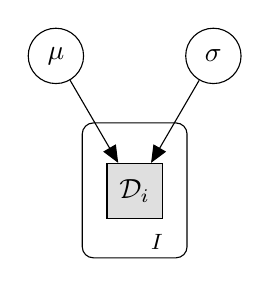
\begin{tikzpicture}[main/.style = {draw, circle, minimum size=8mm,node distance=20mm}]
  % nodes
  \node[obs, rectangle] (D) {${\cal D}_i$};
  \node[latent, above=of D, xshift=-1cm] (mu) {$\mu$};
  \node[latent, above=of D, xshift=1cm] (sigma) {$\sigma$};
  % edges
  \edge {mu, sigma} {D};
  % plates
  \plate[inner sep=0.3cm, yshift=0.2cm, color=black] {} {(D)} {$I$};
\end{tikzpicture}%
\end{minipage}%
\begin{minipage}{.3\textwidth}
 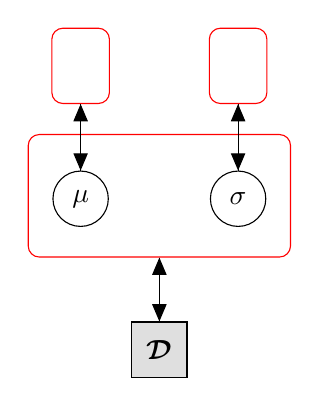
\begin{tikzpicture}[main/.style = {draw, circle, minimum size=8mm,node distance=20mm}]
  % nodes
  \node[obs, rectangle] (D) {$\bD$};
  \node[latent, above=of D, xshift=-1cm, yshift=0.2cm] (mu) {$\mu$};
  \node[latent, above=of D, xshift=1cm, yshift=0.2cm] (sigma) {$\sigma$};
  % plates
  \plate[inner sep=0.0cm, yshift=1.8cm, color=red] {boxOnMu} {(mu)}{};
  \plate[inner sep=-0.0cm, yshift=1.8cm, color=red] {boxOnSigma} {(sigma)}{};
  \plate[inner sep=0.3cm, yshift=0.15cm, color=red] {box} {(mu) (sigma)}{};
  % edges
  \edge {mu} {boxOnMu};
  \edge {boxOnMu} {mu};
  \edge {sigma} {boxOnSigma};
  \edge {boxOnSigma} {sigma};
  \edge {box} {D};
  \edge {D} {box};
\end{tikzpicture}%
\end{minipage}
 \caption{Directed acyclic graph (DAG) of a simple model where the data $\D_i$ with $i = 1, \ldots, I$ follows a normal distribution $\D_i \sim {\cal N}(\mu, \sigma)$. The shaded nodes represent observations. Shown on the left is the classic representation of this model using a DAG. Shown on the right is the \stattools{} representation of this model. The red boxes represent the probability distributions, with the large box around $\mu$ and $\sigma$ being the normal distribution and the two small boxes on top being two prior distributions $\p(\mu)$ and $\p(\sigma)$. The edges represent memory pointers in two directions, pointing from the box above to the node below and vice-versa.}
 \label{fig:easyDAG}
\end{figure}

\subsection{Nodes}
Class \class{TNodeTyped} is a pure virtual base class for \class{TObservation} and \class{TParameter} and defines the common interface of observations and parameters. The most important member variables are:
\begin{itemize}
 \item \privparam{storage}: A storage object. This stores the current and old values of the parameter and manages its dimensions.
 \item \privparam{boxAbove}: A pointer to the box above.
 \end{itemize}

Importantly, \class{TNodeTyped} is templated with a typename \type{Type}. This allows an efficient and flexible memory management. In most cases, the pre-defined types from the library \coretools{} are used, e.g. \type{Probability}, \type{StrictlyPositive} etc. However, a developer is free to implement custom types. In addition, \class{TNodeTyped} is also templated by the number of dimensions. Note that this does not correspond to the size of the parameter (which might not be known at compile time), but to the dimensionality, e.g. two-dimensional. \class{TNodeTyped} inherits from a non-templated base class, \class{TNodeBase}, which implements the interface needed to interact with the parameters/observations from the ``outside'', e.g. for file handling or coordinating the MCMC updates.

We will now go through the different member variables and functions and describe them in more detail. Often, the member variables themselves are classes that contain objects of other classes. We will therefore start at the most basic classes and then explain how other classes make use of them.\\
First of all, it it obvious that every parameter and observation must store its value(s).

\subsubsection{\class{TValueUpdated}}
The class \class{TValueUpdated} is used to store values of parameters. It is templated with \type{Type} and stores the current (\privparam{value}) and old (\privparam{value\_old}) value of the parameter in order to compute the Hastings ratio. It overloads the assignment \pubfunc{operator=}, which swaps \privparam{value\_old} and \privparam{value} and then sets \privparam{value} to the value provided. It further overloads the cast \pubfunc{operator Type} to return the current value.

In constrast to parameters, observations do not need to store old and new value since they are not updated. Observations simply store instances of \type{Type}. The interface for getting and setting however is the same regardless which value type is used: The assignment \pubfunc{operator=} and the cast \pubfunc{operator Type} are defined for both.

\subsubsection{\class{TMultiDimensionalStorage}}
Parameters and observations can be single values, one-dimensional vectors or $n$-dimensional matrices. All these data structures can be stored as a linear vector by transforming a linear index to a multi-dimensional coordinate and vice versa. For example, a 2-dimensional matrix is stored in a linear fashion by pasting row by row together (row-major layout). The main advantages of this design are that 1) this scales to any dimension, as we know how to linearize a $n$-dimensional index and back, 2) this provides a coherent interface, independent of the dimension and 3) if a smart layout is chosen (cache-friendly), it is faster than looking up values in a nested structure.

This concept is implemented in class \class{TMultiDimensionalStorage}. It is templated with the type (\type{Type}) and the number of dimensions (\type{NumDim}) of the underlying storage. It has three important member variables:
\begin{itemize}
 \item A vector of type \type{Type} that stores the values.
 \item An instance of \class{TDimension}, storing the dimensions of these values.
 \item An array of pointers to \class{TNamesEmpty}, where each element in the array stores the names of one dimension.
\end{itemize}
\class{TMultiDimensionalStorage} implements the operator \pubfunc{operator=} that provides access to the values of the parameter. To get linear indices from $n$-dimensional coordinates, \class{TMultiDimensionalStorage} also provides wrapper functions of \class{TDimension} (e.g. \pubfunc{getIndex}, \pubfunc{getRange}, \pubfunc{getFull}, \pubfunc{get1DSlice} etc.). Hence, \class{TMultiDimensionalStorage} manages both values and their dimensionality. \\

Class \class{TMultiDimensionalStorage} provides different options to fill values. If the dimensions are known at run-time, the function \pubfunc{resize} allocates the memory which can then be set with the \texttt{[]} operator.
However, the dimensions might not be known in advance. For example, when reading in data from a file, we typically know the number of columns from the header, but we do not know the number of rows until we have reached the end of the file. We provide special functions for such cases:
\begin{itemize}
 \item Before reading the data, the function \pubfunc{prepareFillData} must be called. This function prepares the memory required to fill the data. The basic idea is that for most input files, all except one dimension are known. For example, in a VCF file, we know from the header how many individuals there will be. However, we will not know how many loci there will be until we parsed the entire file. We might have a guess, but it can be less or more. This function threrefore expects two arguments. The first argument is a guess of the length of the first dimension (i.e. the most outer dimension when linearizing the data, see chapter about dimensions). The second argument is an array of all known dimensions. The guess of the length of the first dimension makes the memory-filling process more efficient, because we reserve the memory in advance (with the vector function \pubfunc{reserve}) and then fill it (with the vector function \pubfunc{emplace{\textunderscore}back}). If we need more memory than guessed, this is not a problem, we will simply \pubfunc{emplace{\textunderscore}back} to the vector.
 \item Then, we can fill the data using \pubfunc{emplace{\textunderscore}back}. Note that data must be filled in an ordered manner (i.e. the way it is supposed to be stored), no re-ordering will be possible afterwards.
 \item When all data has been filled, the function \pubfunc{finalizeFillData} must be called. This function calculates the effective length of the first dimension based on the number of elements that were filled and the known dimensions; and resizes the vector of stored values to its actual size (to release redundant memory).
\end{itemize}


In the following section, we will dive deeper into the concept of linearizing $n$-dimensional arrays and explain how this is implemented in \class{TDimension}.

\paragraph{\class{TDimension}}

\class{TDimension} is templated with the number of dimensions, as this is known at compile time. It stores a array \privparam{dimensions} of size \template{NumDim} that represents the length of each dimension.

When initializing a \class{TDimension} object, the total size of the array (= the product of all dimensions) is automatically calculated and stored in variable \privparam{totalSize}.\\
The linear index $s$ is calculated from a $D$-dimensional array of coordinates $\boldsymbol{n} = n_1, \ldots, n_D$ as
\begin{equation}\label{eq:linearize}
 s = \sum_{i=1}^{D} \left( \prod_{j=i+1}^{D} N_j \right) n_i,
\end{equation}
where $N_j$ corresponds to the length of dimension $j$. To optimize speed, this double-loop is written out for 1-, 2- and 3-dimensional cases, respectively:
\begin{equation*}
 s = n_1 \text{ and } s = n_2 + n_1 N_2 \text{ and } s = n_3 + N_3(n_2 + n_1 N_2).
\end{equation*}
The $D$-dimensional array of coordinates $\boldsymbol{n} = n_1, \ldots, n_D$ is calculated from a linear index $s$ as follows: \label{algo:getSubscripts}
\begin{enumerate}
 \item Start at the most inner dimension $i = D$.
 \item Calculate the index in the current dimension $i$ with $n_i = s \bmod N_i$.
 \item Update the linear index by removing the effect of the current dimension: $s' = \frac{s - n_i}{N_i}$.
 \item Repeat steps 2-3 for next dimension until the most outer dimension is reached.
\end{enumerate}
Again, this algorithm can be written out for speed for 1- and 2-dimensional arrays:
\begin{equation*}
n_1 = s,
\end{equation*}
and
\begin{equation*}
 n_2 = s \bmod N_2 \text{ and } n_1 = \frac{(s - n_2)}{N_2}.
\end{equation*}

Most other functions of class \class{TDimension} use function linearizeIndex to linearize a vector of coordinates, and then return an object of class \class{TRange}. \class{TRange} is a very simple class that consists of three members: \pubparam{begin}, \pubparam{end} and \pubparam{increment}. These correspond to the first index in the linear array, the last (not included) index in the linear array, and the increment one has to use to get the correct elements. It is then straightforward to use \class{TRange} in a for-loop like this:
\begin{lstlisting}
for (size_t i = range.begin; i < range.end; i += range.increment){
 // ...
}
\end{lstlisting}

The following functions are implemented in \class{TDimension}:
\begin{itemize}
 \item \pubfunc{getIndex}: takes a vector of coordinates, and returns the linear index.
 \item \pubfunc{getDiagonal}: only for 2-dimensional square matrices, throws otherwise. Returns a range object for all linear indices of the elements on diagonal.
 \item \pubfunc{getRange}: takes two vectors of coordinates (start and end) and returns a range object of all elements between those.
 \item \pubfunc{get1DSlice}: takes a number \pubparam{dim} and a vector of coordinates, \pubparam{start}. It will start at the linear index of \pubparam{start}, follow the given dimension \pubparam{dim} until its end, and return the corresponding range object. A classic example would be a 2-dimensional matrix, where we want to start at element $\{4,0\}$ (fifth row, first column), and go over all elements of dimension 1 (= columns), to get one full row (end: $\{4,ncol\}$).
 \item \pubfunc{getFull}: returns a range of all linear indices from first to last element, with increment 1.
\end{itemize}

\paragraph{\class{TNamesEmpty}}

As mentioned above, class \class{TMultiDimensionalStorage} stores a vector of pointers to \class{TNamesEmpty}, such that each dimension has a pointer to the dimension names. For example, a three-dimensional parameter will have a vector with three pointers to \class{TNamesEmpty}, corresponding to the dimension names of the first, the second and the third dimension. \class{TNamesEmpty} is a pure virtual base class that provides a common interface to all deriving name classes. The \texttt{[]} operator can be used to get the name as a string for an element with a certain index of a dimension. The following classes derive from it:
\begin{itemize}
 \item \class{TNamesStrings}. This class is nothing more but wrapper of a vector of strings: it provides functions to resize the vector and to add or set elements to it. The \texttt{[]} operator simply returns the element of the vector with the corresponding index. This class is e.g. useful to store sample names or names of covariates.
 \item \class{TNamesIndices}. This class stores only the offset for indices (by default 1, but can be set to zero). The \texttt{[]} operator adds its argument to the offset and returns this result as a string. This is the most simple class, and is typically used for simulating parameters (when there are no specific names), or for parameters whose elements correspond to ``categories'', e.g. the event probabilities from a categorical distribution.
 \item \class{TNamesIndicesAlphabetUpperCase}. This class stores nothing and returns the (numeric) index given to the \texttt{[]} operator as a alphabetic representation in upper case letters of that index in Excel column name stype (i.e. 0 $\to$ A, 1 $\to$ B, \ldots, 25 $\to$ Z, 26 $\to$ AA, 27 $\to$ AB, 51 $\to$ AZ, 52 $\to$ BA etc.)
  \item \class{TNamesIndicesAlphabetLowerCase}. This class stores nothing, but returns the (numeric) index given to the \texttt{[]} operator as a alphabetic representation in lower case letters of that index in Excel column name stype (i.e. 0 $\to$ a, 1 $\to$ b, \ldots, 25 $\to$ z, 26 $\to$ aa, 27 $\to$ ab, 51 $\to$ az, 52 $\to$ ba etc.)
 \item \class{TNamesPositions}. This class stores a pointer to \class{TPositionsRaw}, which is a class that stores a vector of chunk names (as strings) and a vector of positions (as \texttt{uint32{\textunderscore}t}). The \texttt{[]} operator returns a string consisting of chunk name and position (concatenated by some delimiter). This class is useful to store positional information, e.g. chromosome (as chunks) and loci (positions).
\end{itemize}
The idea behind these classes is that the developer reads the observations and creates a name class, depending on which kind of names need to be stored. The name class for each dimension is then given over the function \pubfunc{setDimensionName} to the observation. For example, when reading a VCF-file containing genotype likelihoods, the developer will need to create and fill three such name classes: one for the loci (i.e. \class{TNamesPositions}), one for the individuals (i.e. \class{TNamesStrings}) and one for the genotype (i.e. \class{TNamesIndices}). The developer will then pass them to the instance of the observation class storing these genotype likelihoods. After this, when the storage of the DAG is initialized, the box specified on these data knows how to match its parameter dimensions to the observation dimensions. For example, if one would specify a normal mixed model directly on these genotype likelihoods, the hidden state would be per locus, and would therefore retrieve the pointer to the loci-names from the observations below. When writing to a file, each parameter will hence have the correct dimension names.

\subsection{Observations}
We define observations as the node(s) located at the bottom of the DAG that contain observed data and that are not to be estimated. The class \class{TObservation} represents such an observation. In its constructor, it gets an instance of \class{TMultiDimensionalStorage} that contains the data and that is not modified afterwards.

\class{TObservation} is templated with its type, the number of dimensions and the type of the box above. It inherits from \class{TObservationBase}, which is not templated and provides a pure virtual interface. It further inherits from \class{TNodeTyped}.

\subsection{Parameters}
We define parameters as the node(s) located on the upper levels of the DAG that are to be inferred. The class \class{TParameter} represents such a parameter. Most importantly, \class{TParameter} has functionalities to update itself with Metropolis-Hastings or Gibbs sampling.

\class{TParameter} is templated with typename \type{Spec} that specifies the compile-time features of the parameter, as well as with the type of the box above. \class{TParameter} inherits from \class{TParameterBase}, which is not templated and provides a pure virtual interface. It further inherits from \class{TNodeTyped}.

\subsubsection{\class{ParamSpec}}
This class specifies the compile-time features of a parameter. It is templated with the following mandatory arguments:

\begin{itemize}
 \item \type{typename Type}: The type that defines the interval of the parameter. Can be any of the weak types from \coretools{}, e.g. \type{Unbounded}, \type{Probability}, \type{StrictlyPositive} etc.
 \item \type{Hash<size\_t H>}: A unique hash, generated from the name of the parameter. Used to make each parameter uniquely identifiable.
 \item \type{typename TypeBoxAbove}: The full type of the box above the parameter.
 \end{itemize}

\class{ParamSpec} is futher templated with a template parameter pack (\texttt{\ldots}) that represent optional arguments. Since all of these optional arguments have a unique type identifier, they can be given in any order. If they are not specified, a default value is used.
\begin{itemize}
 \item \type{NumDim<size\_t N>}: The number of dimensions. Default is \texttt{N = 1}.
 \item \type{typename Constraint}: A constraint. Currently supported constraints are \class{Unconstrained}, \class{SumOne} and \class{LengthOne}. Default is \class{Unconstrained}.
 \item \type{Parallelize<MarkovOrder Order>} Indicates if the update of the parameter can be parallelized, and with which Markov order. The template argument \texttt{MarkovOrder} is a \type{enum} with possible values \type{allDependent}, \type{allIndependent} and \type{different}. If \type{allDependent}, all elements in the vector all dependent on each other, such that parallelization is not possible. If \type{allIndependent}, all elements in the vector are independent of each other, such that the update can be fully parallelized among the indices. If \type{different}, there are some dependencies, but they are possibly only known at runtime and must then be provided in the constructor of \type{TParameter}. Default is \texttt{MarkovOrder::allDependent}, resulting in no parallelization.
 \item \type{Weights<size\_t N, UpdateWeights\ldots W>} Update weights, one per dimension. Currently supported weights are \type{regular}, \type{irregular}, \type{geometricUniform}, \type{log10StatePosterior} and \type{powerStatePosterior}. Default is \type{W = regular} for each dimension.
 \item \type{RJMCMC<typename SpecModelParameter>} Whether or not this parameter is an RJ-MCMC parameter. A RJ-MCMC parameter is a parameter that is present or absent in a model, depending on an indicator variable. Default is \type{NoRJMCMC}.
\end{itemize}

\subsubsection{Parameter constraints}

Certain parameter vectors have constraints on their values. We consider two cases. First, a unit vector $\x = \{x_1, \ldots, x_I\}$ has length one, i.e. $\sqrt{\sum_{i=1}^I x_i^2} = 1$. Second, a normalized vector sums to one, i.e. $\sum_{i=1}^I x_i = 1$.

The elements of such parameters can not be updated independently in the MCMC without violating the constraints. There are two options to update constrained parameters: joint and pair-wise. In a joint update, all elements of the parameter are slightly modified and then re-normalized to satisfy the constraint. In a pair-wise update, two elements are updated together such that the constraint is still satisfied.

In the following paragraphs, we will discuss the different updating schemes.

\paragraph{Pairwise update of unit vectors}

Let us denote by $\x = \{x_1, \ldots, x_I\}$ a unit vector such that $\sqrt{\sum_{i=1}^I x_i^2} = 1$. Let us further denote by $i,j$ the two indices that are being updated. A pair-wise update of $x_{i}$ and $x_{j}$ will always result in a valid unit vector $\x'$ if
\begin{equation}\label{eq:condCircle}
 x_{i}^2 + x_{j}^2 = x_{i}'^2 + x_{j}'^2.
\end{equation}

This condition can be solved by representing the problem as a circle where the radius is given by
\begin{equation*}
 r_{ij}(\x) = x_{i}^2 + x_{j}^2.
\end{equation*}

Every value on the circumference of this circle will satisfy the condition given by equation \eqref{eq:condCircle}.

The proposal kernel to get a new value $p_{ij}(\x)' =(x_{i}', x_{j}')$ should be symmetric to avoid extra computations in the Hastings ratio. A computationally cheap and symmetric proposal kernel is to sample a random point along the tangent line to the circle and then normalize its norm to $r_{ij}(\x)$ to project it on the circle.

The slope of the tangent line is given by the vector

\begin{equation*}
 s_{ij}(\x) = \begin{pmatrix}
                 1 \\
                 -\frac{x_{i}}{x_{j}}
                \end{pmatrix},
\end{equation*}

which is normalized to unit length:

\begin{equation*}
 \hat{s}_{ij}(\x) = \frac{s_{ij}(\x)}{|| s_{ij}(\x) ||}
\end{equation*}

We then propose a random jump $\alpha$ according to some proposal kernel and calculate the new values $p_{ij}(\x)'$ as

\begin{equation*}
 p_{ij}(\x)' = \gamma \left( p_{ij}(\x) + \alpha \hat{s}_{ij}(\x) \right),
\end{equation*}

where $\gamma$ is the normalizing ratio

\begin{equation*}
 \gamma = \sqrt{\frac{||p_{ij}(\x)||}{||p_{ij}(\x)'||}} =  \sqrt{\frac{x_{i}^2 + x_{j}^2}{x_{i}'^2 + x_{j}'^2}}.
\end{equation*}

\paragraph{Pairwise update of normalized vector}

Let us denote by $\x = \{x_1, \ldots, x_I\}$ a vector with length one such that $\sum_{i=1}^I x_i = 1$. Let us further denote by $i,j$ the two indices that are being updated. A pair-wise update of $x_{i}$ and $x_{j}$ will always result in a valid vector $\x'$ of length one if
\begin{equation}
 x_{i} + x_{j} = x_{i}' + x_{j}'.
\end{equation}

Since $x_i$ and/or $x_j$ can be very small, we scale the proposal width by the sum $x_{i} + x_{j}$. Specifically, our goal is to propose a jump $u \sim \alpha \sqrt{x_i^2 + x_j^2}$ where $\alpha \sim {\cal N}(0, \sigma)$ and $\sqrt{x_i^2 + x_j^2}$ is the length of the line constituted by all valid $x_i, x_j$ combinations. Given jump $u$, the new values are simply $x_i' = x_i + u$ and $x_j' = x_j - u$. However, we need to make sure to mirror at the maximum given by $x_i + x_j$. To achieve this, we re-formulate the above as:

\begin{equation*}
 x_i' \sim {\cal N}(x_i, \sigma \sqrt{x_i^2 + x_j^2}),
\end{equation*}

where we mirror at $x_i + x_j$. The new value of $x_j'$ is then simply given by $x_j' = x_i + x_j - x_i'$.

\subsubsection{Update weights}

In general, each element of a parameter is updated exactly once per MCMC iteration. However, for certain parameters, we might have a guess about which elements are more relevant than others. These elements should preferrably be updated more often, therefore allocating computational resources to the elements that need fine-tuned updating. This ideally improves convergence of the chain, allowing for shorter MCMCs.

The idea is to allocate update weights to each dimension of a parameter. For example, the first dimension of a parameter is updated according to some specific weights, whereas the second dimension is updated ``regularly'', i.e. each element once. The enum \enum{UpdateWeights} specifies all possible weighting schemes. The parameters of the weighting schemes can be passed as vectors of strings, if necessary, but there are sensible default values for all schemes.

\paragraph{\enum{UpdateWeights::regular}}

Returns equal weights for all indices.

\paragraph{\enum{UpdateWeights::irregular}}

Returns the (untransformed) weights provided by the developer. This is useful if some tool-specific algorithm is used to calculate the weights.

\paragraph{\enum{UpdateWeights::geometricUniform}}

\begin{figure}[t]
\begin{center}
\includegraphics[width=\textwidth]{Figures/updateWeights.pdf}
\end{center}
\caption{Update weights as a function of the input statistics. (A) The weights $Q$ as a function of the input ranks $r$ for \enum{UpdateWeights::geometricUniform}. (B) The weights $Q$ as a function of the input state posterior probabilities $p$ for \enum{UpdateWeights::log10StatePosterior}. (C) The weights $Q$ as a function of the input state posterior probabilities $p$ for \enum{UpdateWeights::powerStatePosterior}. }
\label{fig:updateWeights}
\end{figure}

The input statistics are ranks $r_i$ for all indices $i = 1, \ldots, N$, for instance obtained by the ranking of a statistical test. The weight $Q_i$ of index $i$ is then given by $Q_i = \frac{3}{10}U_i + \frac{7}{10} G_i$, where $U_i$ is a discrete uniform distribution between 1 and $n$, and $G_i = (1-p)^{r_i-1}p$ is the geometric distribution. We determine the parameter $p$ of the geometric distribution based on two probabilities $t$ and $x$, which specify the top fraction $t$ of all elements that receive a fraction $x$ of the effort in updating. By default, $t = 0.2$ and $x = 0.9$, meaning that the top 20\% elements receive 90\% of the updating effort. For $n \to \infty$, the parameter $p$ can be computed as

\begin{equation*}
 p = 1-\exp\left(\frac{\log(1-x)}{tN}\right),
\end{equation*}

by solving the cumulative distribution function for $t$ elements for $p$. It can be shown that this approximation is valid if $n > 150$. Figure \ref{fig:updateWeights}A visualizes the weight distribution for different values of $t$ and $x$.

\paragraph{\enum{UpdateWeights::log10StatePosterior}}

The input statistics are state posterior probabilities $p_i$ for all indices $i = 1, \ldots, N$. The weight $Q_i$ of index $i$ is then given by the absolute logarithmic value of the complement of the state posterior probability:
\begin{equation*}
 Q_i = -\log_{10}(1-p_i),
\end{equation*}

where we cap $p_i$ at 0.01 and 0.99, respectively. The $Q_i$ are normalized such that they sum to one, $\sum_i Q_i = 1$. With this weight distribution, indices with high state posterior probabilities will receive higher update weights (Figure \ref{fig:updateWeights}B).

\paragraph{\enum{UpdateWeights::powerStatePosterior}}

The input statistics are state posterior probabilities $p_i$ for all indices $i = 1, \ldots, N$. The weight $Q_i$ of index $i$ is then given by a power function with the state posterior probability as a base:

\begin{equation*}
 Q_i = m + (1-m) p_i^\beta,
\end{equation*}

where $m$ is an intercept in [0,1] and $\beta$ is the slope (Figure \ref{fig:updateWeights}C). If $\beta = 1$, a linear function results. If $\beta < 1$, a concave function with a flat slope results that levels off for $p_i \to 1$. If $\beta > 1$, a convex function with a steep slope results. By default, $\beta = 0.5$ and $m = 0.1$. The $Q_i$ are normalized such that they sum to one, $\sum_i Q_i = 1$.

\paragraph{\class{TUpdateWeights}}

For each dimension of a parameter, an enum \enum{UpdateWeights} has to be specified at compile time. The update weight of a (multi-dimensional) index is given by the product of the update weights for all dimensions: $Q_i = Q_{\{j_1, \ldots, J_D\}} = \prod_{d=1}^D Q_{j_d}$, where $\{j_1, \ldots, J_D\}$ corresponds to the subscripts of the linear index $i$ in all $d=1, \ldots, D$ dimensions. The class \class{TUpdateWeights} provides several functions that calculate those linear weights and calculate the cumulative of the linear weights, which are ultimately needed for choosing an index to update.

\subsubsection{Choosing indices to update}

As discussed previously, a parameter can be updated regularly, i.e. each index exactly once per iteration, or else according to update weights. In addition, constraints on a parameter dimension may require special update types, such as an update in pairs or a joint update of the entire dimension. Finally, all update functions should be safe to parallelize, i.e. one index should never be updated by two threads at the same time. To achieve this, multiple classes handle each specific combination of cases. Each class implements the function \pubfunc{numUpdates} that specifies the number of updates to perform per iteration. In addition, each class implements the function \pubfunc{pick} that takes the current iteration and thread as arguments, and returns an instance of \class{TRange} that specifies one or multiple indices to updated.

\paragraph{\class{TUpdateSingle}} This class handles updates when there are no constraints and when \enum{UpdateWeights::regular} is used for all dimensions. In this case, each index should be updated exactly once per iteration. The initialization function of this class takes an instance of \class{TMarkovOrder}. This class \class{TMarkovOrder} is described in section \ref{section:MarkovOrder} and defines a range of parameter indices that can be updated independently and thus can be parallelized. There are possibly multiple instances of \class{TUpdateSingle}. Each instance will loop over the indices within its internal range. The function \pubfunc{pick} then transform the internal index to the index of the full parameter space as described in \ref{section:MarkovOrder}.

\paragraph{\class{TUpdateSingleWeighted}} This class handles updates when there are no constraints and when at least one dimension uses non-regular update weights. The class randomly selects an index to update based on the cumulative update weights. If the update is parallelized, we need to make sure that there is no race conditions, i.e. that one index is never updated by two threads simultaneously. To achieve this, we assign a range of indices to one specific thread $t = 1, \ldots, T$ by splitting the vector of cumulative weights into $T$ vectors, one per thread. The function \pubfunc{pick} then draws an index from the cumulative weights of the current thread.

To split the vector, we use a simple splitting scheme that aims at assigning approx. the same cumulative weight to each thread, but making sure that each thread gets at least one index to update. We note that this might not result into the exact weights. For example, if there are three elements with the cumulative weights $\{0.1, 0.2, 1.0\}$ and three threads are used for updating, each element will be assigned to one thread and updated equally often. However, for more indices and a less extreme weight distribution, this becomes less of an issue. Ultimately, the update weights are rough estimates too and should not be problematic if a parameter is updated a bit more or less than the update weights predict.

In addition, as in class \class{TUpdateSingle}, the initialization function takes an instance of \class{TMarkovOrder} to define a subset of indices to update. The weights given to the class are then subsetted to the indices from this sequence.

\paragraph{\class{TUpdatePair}} This class handles updates when \enum{UpdateWeights::regular} is used for all dimensions and when there are constraints such that parameters must be updated in pairs. The template argument \template{AlongDim} specifies the dimension along which the constraint holds. The class \class{TIndexSampler} is used to generate random index pairs with the use of a single random number. This random number corresponds to one random position $i$ and it pairs up with index $j = i+1$. From this, all other pairs are created by shifting $i' = i-1$ and $j' = j+1$ repetitively, where the indices are set to $N-1$ when crossing zero and to zero when crossing $N-1$. The pairwise indices thus run along one dimension, which represents a one-dimensional slice. In the case of $D$ dimensions with length $N_d$ each, there are $K = \prod_{d \neq AlongDim}^D N_d$ such slices. The class \class{TIndexSamplerMultiDim} transforms a linear index in the parameter space into the index relevant for the pairwise index sampler and then back-transforms the index of the pair, corresponding to the index in \template{AlongDim}, into two linear indices in the parameter space. This is thread-safe, since each parameter index occurs at most once within all possible index pairs.

\paragraph{\class{TUpdatePairWeighted}} This class handles updates when at least one dimension uses non-regular update weights and when there are constraints such that parameters must be updated in pairs. The template argument \template{AlongDim} specifies the dimension along which the constraint holds. In this case, we can not simply assign indices to threads as before, since then certain indices will never be assigned to the same pair. To prevent race conditions, we store all the indices that are currently updated in a vector, and only allow a thread to update an index if it is not present in this vector. This section of the code is marked with \texttt{pragma critical} such that only one thread can access it at a time. The first index of a pair is drawn at random from the cumulative update weights. The second index of the pair is then also drawn at random from the cumulative update weights, but ensuring that i) it is located in the same slice as the first index and ii) it is not the same as the first index. To achieve this, we re-scale the cumulative weights in the dimension \template{AlongDim} by excluding the weight of the first index, and drawing at random from these weights.

\paragraph{\class{TUpdateJoint}} This class handles updates when \enum{UpdateWeights::regular} is used for all dimensions and when there are constraints such that all parameters of a certain dimension, given by the template argument \template{AlongDim}, must be updated jointly. In this case, each one-dimensional slice along \template{AlongDim} should be updated exactly once per iteration. Note that in this case we don't allow for update weights.

\subsubsection{Parallelization of updates}\label{section:MarkovOrder}

When parameter indices can be updated independently, their update can be parallelized. The template argument \texttt{MarkovOrder} of the parameter specification is used to define the dependency assumptions.
The three possible enums \type{allDependent}, \type{allIndependent} and \type{different} correspond to no, full and partial parallelization, respectively.

For the \type{different} case, the Markov order must be given at runtime to the constructor of \class{TParameter}. In general, a Markov order of $X$ means that every $(X+1)^{th}$ element can be updated independently. For example, a Markov order of zero corresponds to full independence of elements as every element can be updated independently. A Markov order of one corresponds to the classic HMM case where every second element can be updated independently, as the update of one index only depends on the direct neighbours. The largest possible Markov order is the size of the parameter minus one, which corresponds to full dependency.

This concept can be generalized to multiple dimensions where each dimension is assigned a Markov order.

\begin{figure*}[t]
\begin{center}
\includegraphics[width=0.8\textwidth]{Figures/picker.pdf}
\end{center}
\caption{Two examples of Markov orders for a two-dimensional parameter with seven rows and five columns. The colors represent the index pickers, and the numbers represent the index within the index picker. (A): Markov order = (1, 2) results in six index pickers of different dimensions. (B): Markov order = (6, 0) results in seven index pickers, one for each row.}
\label{fig:picker}
\end{figure*}

Having specified the Markov order, the challenge is then to parallelize the loop over indices while respecting the Markov order. To simplify the problem, we currently only allow for parallelization in unconstrained parameters, i.e. if either of the classes \class{TUpdateSingle} or \class{TUpdateSingleWeighted} are used to pick indices to update. We then define a vector of pickers that corresponds to multiple instances of these two classes. Each picker is assigned to a subset of all parameter indices that can be fully parallelized. In the function \pubfunc{update} of \class{TParameter}, we first loop over all pickers, which is never parallelized. We then loop over all indices within one picker, which is fully parallelized using \texttt{OpenMP}.

The class \class{TMarkovOrder} manages the compression of full indices to picker indices and their expansion back to full indices. Let us define by $\m = (m_1, \ldots, m_D)$ the $D$-dimensional Markov order and by $\f = (f_1, \ldots, f_D)$ the dimensions of the parameter.

The number of pickers $P$ is given by
\begin{equation*}
 P = \prod_{d=1}^D n_d,
\end{equation*}

where $n_d = m_d + 1$ denotes the Markov order $m_d$ increased by one.
Each picker $p = 1, \ldots, P$ is then assigned a starting value. This is obtained by calculating the $D$-dimensional coordinates $\s_p$ of the linear index $p$ in the space spanned by $\n = (n_1, \ldots, n_D)$ as explained in section \ref{algo:getSubscripts}. This is visualized in Figure \ref{fig:picker}. The internal dimensions $\q_p = (q_{p1}, \ldots, q_{pD})$ of each picker $p$ are then given by

\begin{equation*}
 q_{pd} = \ceil[\bigg]{\frac{f_d - s_{pd}}{n_d}},
\end{equation*}

for each dimension $d$. This simply corresponds to the total length of the dimension when starting at $s_{pd}$, divided by the step size $n_d$, and then rounding up.

To transform internal index $i$ of picker $p$ to the index $j$ in the full parameter space, we first transform the linear index $i$ to the $D$-dimensional coordinates $\k = (k_1, \ldots, k_D)$ in the space spanned by $\q_p$. We then expand these coordinates to the full space using

\begin{equation}\label{eq:expandPicker}
 k_{d}' = s_{pd} + k_d * n_d,
\end{equation}

for each dimension $d$. This simply corresponds to multiplying the index $k_d$ by the step size $n_d$ and adding the starting value $s_{pd}$ to it. The linear index $j$ is then obtained by linearizing the coordinates $\k'$ using \eqref{eq:linearize}.

We consider the special case that all elements are independent. In this case, there is a single picker and the equation \eqref{eq:expandPicker} simplifies $j=i$.

Finally, it would be quite inefficient if all indices had their own picker when all indices are dependent, i.e. if the enum \type{allDependent} is used (which is the default). In this case, class \class{TParameter} sets the Markov order to all zeros, which results in a single picker. Using compile-time statements, it is ensured that the number of threads for parallelization is restricted to one, which makes the use of this single picker safe to use.

\subsubsection{Proposing new values}
We have now seen the different mechanisms on how indices are selected for an update. In the following section, we will describe on how the update is effectively performed for the selected indices. The base class for this is \class{TUpdateTypedBase} that manages the Metropolis-Hastings update of the parameter value. It holds a pointer to a proposal kernel that proposes a new value based on some proposal width.

Class \class{TUpdateTypedBase} is templated and its type matches the type of the parameter. The proposal widths, however, are of the underlying type (and not of the type itself). The reason is that for certain custom types, e.g. for strictly negative values, the proposal width could only hold negative values - but this is clearly not useful, since we would have to implement a special proposing scheme for such types.

After each burnin, \class{TUpdateTypedBase} is responsible for:
\begin{enumerate}
 \item Adjust the jump size $j$ by calculating
 \begin{equation*}
  j' = ju,
 \end{equation*}
 with
 \begin{equation}\label{eq:scalePropWidth}
  u = \left(\frac{(a+1)}{r(T+1)} \right)
 \end{equation}

 where $a$ is the number of accepted updates, $T$ is the number of total updates and $r$ is the ideal acceptance rate. We add one to avoid issues if the parameter has never been accepted. By default, $r$ is set to 0.44, since this appears to be the optimal acceptance rate for the Metropolis-within-Gibbs algorithm where a single coordinate is updated at a time \citep{brooks2011}. However, $r$ can be overridden by providing the command-line argument \texttt{accRate}.

 \item Clear all counters (the number of accepted and total updates).
\end{enumerate}

Its derived classes implement different options on how the proposal widths are handled.

\paragraph{\class{TUpdateShared}}
The class \class{TUpdateShared} inherits from \class{TUpdateTypedBase} and uses the same proposal width for all indices of parameters. This is useful if the parameter values are approx. the same order of magnitude.

\paragraph{\class{TUpdateUnique}}
The class \class{TUpdateUniqueRegular} inherits from \class{TUpdateTypedBase} and uses a proposal width that is specific to each parameter index. This is useful if the parameter values are of different orders of magnitude, such that using the same proposal width for all will result in poor mixing for some elements. The class is templated with \template{Regular} that indicates if the update weights are all regular. If all weights are regular, each index is updated equally often, so the total number of updates can be a single number. If the weights are not regular, indices might be updated more often than others, therefore, the total counter of updates must run per index.

\subsubsection{\class{TPropKernelBase}}
The actual proposal of a new value uses a certain proposal distribution. This is handled by the class \class{TPropKernelBase} and its derived classes.

Proposal kernels 1) propose a value $j$ according to some distribution, 2) add it to $x$, and 3) mirror. All proposal kernels must restrict the value of $j$, in order to prevent too large jumps that could cause overshooting or numerical issues. We therefore make sure that the proposal width $\delta$ is always smaller than half of the value's range $r$, $\delta \leq \frac{r}{2}$.
All of the following proposal kernels except \class{TPropKernelScalingLogNormal} are symmetric and cancel out in the Hastings ratio.

\paragraph{\class{TPropKernelUniform}}
 Uniform proposal kernel where $j \sim {\cal U}(\delta)$. A jump is obtained with $j = R \delta - \frac{\delta}{2}$, where $R$ is a random uniform number between 0 and 1. This is enabled for floating point types.

\paragraph{\class{TPropKernelNormal}}
Normal proposal kernel where $j \sim {\cal N}(0, \delta^2)$. A jump is obtained by drawing random normal values inside a while-loop until $-\frac{r}{2} \leq j \leq \frac{r}{2}$. This is enabled for floating point types.

\paragraph{\class{TPropKernelRandomInteger}}
Integer proposal kernel with random sampling. The new value is randomly sampled from the entire range of the type. This class thus does not have a proposal width that is adjusted. It is designed for integral types with small ranges (e.g. categorical variables) where a proposal width is not meaningful (e.g. a update $0 \to 1$ should be equally likely as an update $0 \to 10$). Per default, this proposal kernel is used for types with a maximum value smaller or equal than 10.

\paragraph{\class{TPropKernelInteger}}
Integer proposal kernel where $j \sim {\cal U}(-\delta, \delta)$. A jump is obtained by randomly picking any value in the range $0, 1, 2, \ldots, 2\delta$. The values are then shifted by $\delta$ in order to be symmetric. If $j=\delta$ is picked, we draw again, since this would result in no update after shifting. If mirroring results in the same value as before, we also draw again. Note that this update has a bad performance for integers with small ranges (e.g. categorical variables), since it requires mirroring which might be quite an overhead for small ranges. For these cases, we instead recommend \class{TPropKernelRandomInteger}.

\paragraph{\class{TPropKernelBool}}
Boolean proposal kernel: $x' = 1-x$. We always propose the opposite value for bools, so jump sizes $j$ do not matter. This is enabled for bools only.

\paragraph{\class{TPropKernelScalingLogNormal}}
A special log-normal proposal kernel that scales with magnitude of value. In general, a desired feature of a proposal kernel is that its width scales with the value $x$ of the parameter that is updated: If $x$ is very small, the proposal width should also be very small. If $x$ is very large, the proposal width should also be very large. However, tuning the proposal width until it matches the value of $x$ might take quite a few iterations, especially if the values of $x$ are very large. A typical solution for this is to update $x$ in the log-space. However, updating $x$ in the log-space is sometimes unpractical, as this naturally imposes a exponential prior with rate 1 on the parameter, which is sometimes too strong.

We therefore implemented a proposal kernel that scales with the value of $x$. We obtain a new value $x'$ by multiplying a jump value j:

\begin{equation*}
 x' = jx,
\end{equation*}

where $j$ follows a log-normal distribution: $j \sim \mbox{Lognormal}(0, \sigma^2)$. In fact, one can show that $x' = jx \sim \mbox{Lognormal}(\log x, \sigma^2)$.

Unfortunately, this proposal kernel is not reversible:

\begin{eqnarray*}
 \p(x' | x) &=& \p(x | x') \\
 \frac{1}{x' \sqrt{2\pi\sigma^2}} \exp \left(-\frac{(\log x' - \log x)^2}{2\sigma^2} \right) &=& \frac{1}{x \sqrt{2\pi\sigma^2}} \exp \left(-\frac{(\log x - \log x')^2}{2\sigma^2} \right) \\
 x &=& x'
\end{eqnarray*}

The ratio of the proposal kernels does not cancel out in the Hastings ratio. We need to correct the Hastings ratio with:

\begin{equation*}
 h = \frac {\p(x | x')}{\p(x' | x)} = \frac{x'}{x}.
\end{equation*}

It is important to note that this proposal kernel does only make sense for strictly positive or strictly negative values, since a sign change is not possible ($j$ will always be positive, therefore $x'$ will always keep the sign of $x$).

Since the proposal kernel is not reversible, using it to infer bounded parameters by mirroring at those boundaries is also more complicated. Mirroring for reversible proposal kernels is valid because

\begin{equation*}
 \p(x|x') + \p(2a -x | x') + \p(2b - x | x') = \p(x'|x) + \p(2a -x' | x) + \p(2b - x' | x)
\end{equation*}

In our case, however, the distances to the proposed values are not the same. We could correct for this in the Hastings ratio, too, but we decided not to implement this, since it was not needed in our use-case. The proposal kernel is anyways automatically ``mirrorred'' at zero, as explained above.

The procedure to adjust the proposal width is also different than for the standard proposal kernels. The variance of $j$ is given by the variance of a log-normal distribution with $\mu = 0$:

\begin{equation*}
 \mbox{Var}(j) = \left(e^{\sigma^2} - 1\right) e^{\sigma^2} = \left( e^{\sigma^2} \right)^2 - e^{\sigma^2}.
\end{equation*}

Our goal is to adjust the variance of the log-normal distribution, $\sigma^2$, according to the factor $u$ from equation \ref{eq:scalePropWidth}:

\begin{equation*}
u \left( \left( e^{\sigma^2} \right)^2 - e^{\sigma^2} \right) = \left( e^{{\sigma^2}'} \right)^2 - e^{{\sigma^2}'}.
\end{equation*}

Solving for ${\sigma^2}'$ results in:

\begin{equation*}
{\sigma^2}' = \log \frac{1}{2} + \log \left(1 + \sqrt{1+4u\left(e^{2\sigma^2} - e^{\sigma^2} \right)} \right).
\end{equation*}

\subsubsection{\class{TMirror}}
Let us have a closer look on how we make sure that the proposed values are inside a specific interval. All types in the framework are weak types from \texttt{coretools} that are defined on a specific interval. By default, this interval is given by the numeric limits of the underlying type. A couple of classes exist that implement the most common non-default intervals, such as positive, strictly positive, the open interval between 0 and 1, the closed interval between 0 and 1, etc. All of these types can return their minimum and maximum value, denoted here by $a$ and $b$, respectively.

In its most basic form, mirroring works like this:
\begin{equation}\label{eq:mirroring}
 \tilde{x} = x+j; \quad x' = \begin{cases}
                                               \tilde{x} \quad &\mbox{if } a \leq \tilde{x} \leq b \\
                                               2a-\tilde{x} \quad &\mbox{if } \tilde{x} < a\\
                                               2b-\tilde{x} \quad &\mbox{if } \tilde{x} > b
                                              \end{cases},
\end{equation}
where $\tilde{x}$ is an initial proposal, and $x'$ is the value returned from the mirroring function. This only holds if $2a-\tilde{x} < b$ and $2b-\tilde{x}>a$ in all cases, so we need to make sure that $\tilde{x}$ is not too large (i.e. by restricting the maximal jump value $j$ to half of the range). However there are different challenges associated with mirroring. A first challenge for both signed and unsigned types arises from the fact that we will run into numeric problems when using equation \eqref{eq:mirroring} for boundaries where $a$ and/or $b$ are given by the numeric limits of that type. If we first add $x+j$ and then mirror, we might have crossed the numeric limits already, but never notice it, as numeric overflow results in undefined behaviour. Hence, we must \textit{first} check if we cross the boundaries, and only \textit{after} do the addition. Note that the following rules apply to both default and non-default min and max.\\
We exceed the minimum if
\begin{equation}\label{eq:mirrorAtMin}
 -j > x - a,
\end{equation}
because the distance between the minimum and the current value is smaller than the jump size. If this is the case, we need to mirror, using the logic of \eqref{eq:mirroring}. However, calculating $2a$ might also result in numeric overflow, so we use the un-simplified equation $a - j - (x - a)$ in order to mirror.
The same logic applies for mirroring at the maximum $b$. We exceed the maximum if
\begin{equation}\label{eq:mirrorAtMax}
 j > b - x,
\end{equation}
because the distance between the maximum and the current value is smaller than the jump size. We then mirror with $b - (j - (b - x))$, as $2b$ would again result in numeric overflow.

For signed types, an additional challenge arises from the fact that adding/subtracting value with different signs can cause numeric overflows, since the value to store this range might be larger than the numeric maximum of the type. This issue is addressed in class \class{TMirrorSigned}, a class for mirroring signed types. If $x\geq0$ and $a<0$, we can safely compute $x-a$ if
\begin{equation*}
 x \leq a - \text{numeric{\textunderscore}min}.
\end{equation*}
If this is not the case, we do not need to care about mirroring anyways, as we restrict $j$ to half of the range, and will therefore never make such a big jump.
For mirroring at the maximum, we would again run into numeric overflow if $b\gg0$ (e.g. the numeric maximum) and $x<0$. We can safely compute $b-x$ if
\begin{equation*}
 -x \leq \text{numeric{\textunderscore}max} - b.
\end{equation*}
If this is not the case, we don't need to care about mirroring as well.\\

For unsigned types (e.g. uint8{\textunderscore}t, uint16{\textunderscore}t etc.), we do not have these range-overflow issues, as the numeric minimum is always 0. Therefore, class \class{TMirrorUnsigned} provides an implementation for unsigned types. The challenge for unsigned types is that we can not directly pass the jump size as an unsigned integer to the function, since unsigned values can't be negative, and if we passed $j$ as an unsigned type, we would always increase $x$ - clearly not what we want. We therefore pass both the jump size as well as the shift to the function for unsigned types (both as unsigned integers), and calculate whether we will jump to the right or the left and mirroring accordingly.\\

A last caveat are integer types. If we applied the above procedure to an integer type, we would need to correct for a non-symmetric proposal kernel in the Hastings ratio because of mirroring. As an example, consider an integral type with an interval $[0,2]$ with possible jumps $\{-2, -1, 0, 1, 2\}$. There are two possibilities to propose the update $0 \to 1$: Either by taking jump $1$ or by taking jump $-1$ and then mirroring at $a = 0$. However, there is only one possibility to propose the reversed update $1 \to 0$, as this is only possible by taking jump $-1$, but not by mirroring.

We solve this issue by mirroring at $a-\frac{1}{2}$ and at $b+\frac{1}{2}$ instead of mirroring at $a$ and $b$. This results in a symmetric, reversible proposal kernel. Since $2\left(a-\frac{1}{2}\right) - \tilde{x} = 2a - \tilde{x} - 1$ and analogously $2\left(b+\frac{1}{2}\right) - \tilde{x} = 2b - \tilde{x} + 1$, we can simply subtract or add one after mirroring at the left or the right boundary, respectively.

\subsubsection{RJ-MCMC}

Reversible-jump MCMC (RJ-MCMC, \citet{green1995}) allows for MCMC updates of parameters that differ in dimensionality. In such cases, the Hastings ratio must account for the change in dimensionality as comparing densities of parameters of different dimensions is meaningless. This is relevant in the case of model choice, e.g. in mixture models. We refer to \citet{Wegmann2019} for a general description of RJ-MCMC. In \stattools{}, we currently allow for a mixed model that consists of two nested submodels $\cM_1 \subset \cM_2$ where both models share the parameters $\btheta$ but model $\cM_2$ has additional parameters $\bsigma$. To compensate for the difference in dimensionality, we use a random vector $\u$ with density $\pi(\u)$ and of the same dimension as $\bsigma$. For the diffeomorphism $\Phi_{12}$ we choose the identity map $(\btheta,\u) \mapsto (\btheta, \bsigma = \u)$ whose Jacobian determinant is $1$ and thus cancels out in the Hastings ratio. The simplified Hastings ratio is then given by
$$
h(\btheta \to (\btheta, \bsigma))=\min\left\{1,\frac{\p(\D|\btheta, \bsigma)\p(\bsigma)\p(\cM_2)q_{21}}{\p(\D|\btheta)\p(\cM_1)\pi(\bsigma)q_{12}}\right\}
$$
for the jump from $\cM_1$ to $\cM_2$ and
$$
h((\btheta,\bsigma) \to \btheta)=\min\left\{1,\frac{\p(\D|\btheta)\p(\cM_1)\pi(\bsigma)q_{12}}{\p(\D|\btheta, \bsigma)\p(\bsigma)\p(\cM_2)q_{21}}\right\}
$$
for the reverse jump. Here, $q_{12}$ denotes the proposal probability for the jump from $\cM_1$ to $\cM_2$, and $q_{21}$ denotes the reverse probability. We fix $q_{12} = 1$, meaning that we will always propose a jump $\cM_1 \to \cM_2$. The reverse probability is set to $q_{21} = 0.1$ by default (and can be changed in the \class{TParameterDefinition}), meaning that in 10\% of the cases we will propose a jump $\cM_2 \to \cM_1$. In all other cases, we will remain in model $\cM_2$ and perform a standard Metropolis-Hastings update of parameter $\bsigma$ instead. We generally recommend to set $q_{21}$ to rather small values, as this choice allows for a sampling rate of $\bsigma$ that is comparable to that of other parameters. If $q_{21}$ was set to high values most updates would correspond to a model jump, and the MCMC would need to run much longer in order to generate sufficiently many posterior samples of $\bsigma$ for parameters where the $\cM_2$ is preferred. $q_{21} = 0.1$ is an arbitrary choice but performed well in our application of RJ-MCMC.

The RJ-MCMC update is implemented as follows. For each RJ-MCMC parameter $\sigma_i$ with $i = 1, \ldots, I$ there exists an indicator variable $m_i$ that is one if $\sigma_i$ is in model $\cM_2$ and zero otherwise. Both parameters $\bsigma = (\sigma_1, \ldots, \sigma_I)$ and $\m = (m_1, \ldots, m_I)$ are instances of \class{TParameter}. In the parameter specification \class{ParamSpec} of $\bsigma$, the user must indicate that this is an RJ-MCMC variable with the parameter specification of $\m$ as a template argument. In addition, the proposal distribution for proposing new values of $\bsigma$ after jumping from $\cM_1 \to \cM_2$ must be specified. This can be any distribution from \texttt{coretools::probdist}. For example, for a $\bsigma$ that is bounded in the interval $(0,1)$, the \type{ParamSpec} for $\bsigma$ should specify \type{RJMCMC<SpecM, coretools::probdist::TBetaDistr>}. Note that the model parameter $\m$ does not need the RJ-MCMC specification in \type{ParamSpec}.

The function \type{calculateLLRatio(SpecSigma)} for $\bsigma$ is then used to calculate the likelihood ratio of the standard Metropolis-Hastings update in case of no jump between submodels.

The function \type{calculateLLRatio(SpecM)} for $\m$ is used to calculate the likelihood ratio of the jump between models. The user needs to figure out which model jump was performed. The jump $\cM_2 \to \cM_1$ would result in \type{m->value(i) == 0}, meaning that the likelihood ratio $\frac{\p(\D|\btheta)}{\p(\D|\btheta, \bsigma)}$ must be calculated. Analogously, the jump $\cM_10 \to \cM_2$ would result in \type{m->value(i) == 1}, meaning that the likelihood ratio $\frac{\p(\D|\btheta, \bsigma)}{\p(\D|\btheta)}$ must be calculated. The other parts of the RJ-MCMC Hastings ratio are evaluated internally in \stattools{}.

\subsection{Prior distributions}
In a Bayesian setting, every parameter is assumed to follow a prior distribution. The prior distribution reflects the knowledge about the parameter before any observations are taken into account. The prior can be an uniform distribution, giving equal weight to every value, or something more sophisticated like a normal, exponential or beta distribution. The latter distributions are parametrized with prior parameters (e.g. mean and variance for the normal distribution).

The relationship between an observation and a parameter is formally called the likelihood. However, from a programming point of view, the implementation of likelihood and prior is the same, as they both define a probabilistic relationship. The following classes, although named ``prior'', equally apply to likelihood functions if they relate an observation to a parameter.

In \stattools{}, the prior distributions are implemented in the classes deriving from \class{prior::TBase}. A couple of prior classes have fixed prior parameters that are not inferred. These all include the name ``Fixed''. Other prior classes infer their prior parameters (and are hence called ``Inferred'').

For efficient calculations, the prior classes must know 1) the type and the number of dimensions of the parameter they are defined on, and 2) the full parameter specification (\class{ParamSpec}) of all prior parameters. The number of templates is thus specific for each prior class. There are certain restrictions on these parameter types, since most priors are only valid on specific intervals. For example, for \class{prior::TNormalInferred} mentioned before, \type{Type} and \type{SpecMean::value\_type} must be unconstrained floating point numbers (constraints are not allowed, since this would represent a truncated normal prior that needs to normalize its densities). \type{ SpecVar::value\_type} on the other hand must be a strictly positive floating point number. To enforce these conditions, the prior classes are all templated with static asserts, such that compile errors result if the conditions are not met.

\paragraph{Initialization}

Prior classes that have inferred prior parameters expect pointers for each such parameter in the constructor. Priors with fixed prior parameters accept a string that contains the values for the prior parameters (seperated by commas). This is handy since users are allowed to change these values over the command-line or via files.

A prior that manages inferred prior parameters usually has certain expectations on the dimensionality of these prior parameters. For instance, a normal prior knows that the parameter for the mean must be a single element, whereas a multivariate normal prior knows that the parameter for the mean must be $D$-dimensional. The function \pubfunc{initialize} of a prior goes over all parameters on which the prior is defined and extracts the necessary information about their dimensions (e.g. the multivariate normal prior will derive the number of dimensions $D$ from the parameter below). The function then calls \pubfunc{initStorage} of each prior parameter, and passes a vector of dimensions, for example \texttt{\{D\}} to it. The parameter then allocates the requested memory.

An important member of class \class{TPriorBase} is a vector of pointers to the data of the parameters and observations it is defined on (member variable \privparam{storageBelow}). Usually, this vector will have only one element, as most parameters have their own prior. However, there might be cases where multiple parameters/observations share the same prior and where the prior parameters should be leared based on all of these parameters/observations.

\subsubsection{Prior ratios}
An important part of a prior is the calculation of prior probabilities. The Hastings ratio for an update of parameter $x \to x'$ is calculated as
\begin{equation*}
 h_x = \min \left(1, \frac{\p(\bD|x') \p(x') q(x', x)}{\p(\bD|x) \p(x) q(x, x')}\right).
\end{equation*}
Here, $\p(\bD|x)$ is the likelihood, $\p(x)$ is the prior probability, and $q(x, x')$ is the proposal kernel. The prior ratio $p_x$, which is the focus of this section, is therefore part of the full Hastings ratio and defined as:
\begin{equation*}
 p_x = \frac{\p(x')}{\p(x)}.
\end{equation*}

As these probabilities can become very small, we usually calculate the log prior ratio:
\begin{equation*}
\log p_x = \log \p(x') - \log \p(x).
\end{equation*}
Here, the prior density $\p(x)$ obviously depends on the prior distribution chosen. The interface to get $\log \p(x')$, $\log \p(x)$ and $\log p_x$ however is the same for all prior distributions:
\begin{itemize}
\item \texttt{getDensity(const Storage \& x, size\_t i)}: Calculates $\p(x_i')$.
\item \texttt{getLogDensity(const Storage \& x, size\_t i)}: Calculates $\log \p(x_i')$.
\item \texttt{getLogDensityRatio(const UpdatedStorage \& x, size\_t i)}: Calculates $\log p_{x_{i}}$.
\end{itemize}

The functions \pubfunc{getDensity} and \pubfunc{getLogDensityRatio} are pure virtual and must be overridden by any prior inheriting from \class{TPriorBase}. The function \pubfunc{getLogDensity} by default just calculates \texttt{log(getDensity())}, but can also be overridden if necessary.

Multiple classes inherit from \class{TPriorBase} and implement specific prior distributions. We will now discuss those in more detail.

\subsubsection{Priors with fixed parameters}

The following paragraphs describe prior distributions where the prior parameters are fixed, i.e. they are not inferred in the MCMC.
\paragraph{\class{prior::TUniformFixed}}
A uniform prior does not have any parameters, except for a minimal and maximal value for which the log density is defined. These values are directly obtained from the underlying type.

The log prior density of a value $x$ with minimum $a$ and maximum $b$ is:
\begin{equation*}
 \log \p(x|a, b) = \log\left(\frac{1}{b-a}\right).
\end{equation*}

The log prior ratio is zero, as every value is equally likely:
\begin{equation*}
 \log p_x = \log \left( \frac{\p(x'|a, b)}{\p(x|a, b)} \right) = 0.
\end{equation*}

\paragraph{\class{prior::TNormalFixed}}

A normal distribution is parametrized by:
\begin{itemize}
 \item mean $\mu$ (\privparam{mean}).
 \item variance $\sigma^2$ (\privparam{var}), where $\sigma^2 > 0$.
\end{itemize}

The log prior density of a value $x$ is:
\begin{equation}\label{eq:priorDensNormal}
 \log \p(x|\mu, \sigma^2) = -\frac{1}{2}\log(\sigma^2) - \frac{1}{2}\log(2\pi) - \frac{1}{2\sigma^2}(x - \mu)^2.
\end{equation}

The log prior ratio is:
\begin{equation}\label{eq:priorRatioNormal}
 \log p_x = \log \left( \frac{\p(x'|\mu, \sigma^2)}{\p(x|\mu, \sigma^2)} \right) =  \frac{1}{2\sigma^2}\left((x - \mu)^2 - (x' - \mu)^2\right).
\end{equation}

\paragraph{\class{prior::TExponentialFixed}}
An exponential distribution is parametrized by:
\begin{itemize}
 \item rate $\lambda$ (\privparam{lambda}), where $\lambda > 0$.
\end{itemize}

The log prior density of a value $x$ is:
\begin{equation}\label{eq:priorDensExponential}
 \log \p(x|\lambda) = \log(\lambda) - \lambda x.
\end{equation}

The log prior ratio is:
\begin{equation}\label{eq:priorRatioExponential}
 \log p_x = \log \left( \frac{\p(x'|\lambda)}{\p(x|\lambda)} \right) = \lambda (x - x').
\end{equation}

\paragraph{\class{prior::TGammaFixed}}
An gamma distribution is parametrized by:
\begin{itemize}
 \item shape $\alpha$ (\privparam{alpha}), where $\alpha > 0$.
 \item rate $\beta$ (\privparam{beta}), where $\beta > 0$.
\end{itemize}

The log prior density of a value $x$ is:
\begin{equation}\label{eq:priorDensGamma}
 \log \p(x|\alpha, \beta) = \alpha \log(\beta) - \log\Gamma(\alpha) + (\alpha - 1) \log(x) - \beta x.
\end{equation}

The log prior ratio is:
\begin{equation}\label{eq:priorRatioGamma}
 \log p_x = \log \left( \frac{\p(x'|\alpha, \beta)}{\p(x|\alpha, \beta)} \right) = (\alpha - 1) \log\left(\frac{x'}{x}\right) + \beta (x - x').
\end{equation}

\paragraph{\class{prior::TChisqFixed}}
A chi-square distribution is parametrized by
\begin{itemize}
 \item the degrees of freedom $k$ (\privparam{k}), where $k > 0$.
\end{itemize}

The log prior density of a value $x$ is:
\begin{equation}\label{eq:priorDensChisq}
 \log \p(x|k) = -\frac{k}{2} \log 2 - \ln \Gamma\left(\frac{k}{2}\right) + \left(\frac{k}{2} - 1 \right) \log x - \frac{x}{2}.
\end{equation}

The log prior ratio is:
\begin{equation}\label{eq:priorRatioChisq}
 \log p_x = \log \left( \frac{\p(x'|k)}{\p(x|k)} \right) = \left( \frac{k}{2} - 1 \right) (\log x' - \log x) + \frac{x - x'}{2}.
\end{equation}

\paragraph{\class{prior::TMultivariateChisqFixed}}
In this prior, $\boldsymbol{x}$ is a vector of $N$ values, and on every element $x_i$ a chisq prior with a different degree of freedom $k_i$ is specified. A classic example is that the degrees of freedom are given by the index $i$ with $N+1-i$, such that the first element in the vector has $N$ degrees of freedom, the second has $N-1$, \ldots, and the last has 1 degree of freedom.\\
Hence, this prior is parametrized by
\begin{itemize}
 \item A vector of degrees of freedom, $\boldsymbol k$ (\privparam{k}), where all $k_i>0$.
\end{itemize}
The log prior density and ratio of a value $x$ are given by \eqref{eq:priorDensChisq} and \eqref{eq:priorRatioChisq}, with the only difference that $k$ depends on the index $i$.

\paragraph{\class{prior::TMultivariateChiFixed}}
In this prior, $\boldsymbol{x}$ is a vector of $N$ values, and on every element $x_i$ a chi prior with a different degree of freedom $k_i$ is specified. A classic example is that the degrees of freedom are given by the index $i$ with $N+1-i$, such that the first element in the vector has $N$ degrees of freedom, the second has $N-1$, \ldots, and the last has 1 degree of freedom.\\
Hence, this prior is parametrized by
\begin{itemize}
 \item A vector of degrees of freedom, $\boldsymbol k$ (\privparam{k}), where all $k_i>0$.
\end{itemize}

The log prior density of a value $x$ is:
\begin{equation*}
 \log \p(x|k) = -\left(\frac{k}{2} - 1\right) \log 2 - \ln \Gamma\left(\frac{k}{2}\right) + \left(k - 1 \right) \log x - \frac{x^2}{2}.
\end{equation*}

The log prior ratio is:
\begin{equation*}
 \log p_x = \log \left( \frac{\p(x'|k)}{\p(x|k)} \right) = \left(k - 1 \right) (\log x' - \log x) + \frac{x^2 - {x'}^2}{2}.
\end{equation*}

\paragraph{\class{prior::TBetaFixed}}
A beta distribution is parametrized by
\begin{itemize}
 \item shape $\alpha$ (\privparam{alpha}), where $\alpha > 0$.
 \item shape $\beta$ (\privparam{beta}), where $\beta > 0$.
\end{itemize}

The log prior density of a value $x$ is:
\begin{equation}\label{eq:priorDensBeta}
 \log \p(x|\alpha, \beta) = \ln \Gamma(\alpha + \beta) - \ln \Gamma(\alpha) - \ln\Gamma(\beta) + (\alpha - 1) \log x + (\beta - 1) \log(1-x),
\end{equation}
where $\ln \Gamma$ is the log-gamma function.
The log prior ratio is:
\begin{equation}\label{eq:priorRatioBeta}
 \log p_x = \log \left( \frac{\p(x'|\alpha, \beta)}{\p(x|\alpha, \beta)} \right) =  (\alpha - 1) (\log x' - \log x) + (\beta-1) (\log(1-x') - \log(1-x)).
\end{equation}

\paragraph{\class{prior::TBinomialFixed}}
A binomial distribution is parametrized by
\begin{itemize}
 \item the success probability for each trial, $p$ (\privparam{p}), where $0 < p < 1$.
\end{itemize}

The data on which a binomial prior is defined must be 2-dimensional, as we allow for different number of trials $n$. The function \pubfunc{setFixedPriorParameters} checks if 1) the data is one-dimensional with a total size of 2 ($n$ and $k$) or if 2) the data is two-dimensional with the number of columns (the second dimension) being exactly two ($n$ and $k$). If neither of these is the case, an error is thrown.

The log prior density of a value $k$ is:
\begin{equation}\label{eq:priorDensBinomial}
 \log \p(k|n, p) = \log { n \choose k} + k\log p + (n-k) \log (1-p).
\end{equation}
The log prior ratio is:
\begin{equation}\label{eq:priorRatioBinomial}
 \log p_k = \log \left( \frac{\p(k'|n, p)}{\p(k|n, p)} \right) =  \log { n \choose k'} - \log { n \choose k} + (k'-k)\log p + (k-k') \log (1-p).
\end{equation}

\paragraph{\class{prior::TNegativeBinomialFixed}}
The negative binomial distribution models the number of failures which occur in a sequence of Bernoulli trials before a target number of successes is reached. Note that there exist different formulations for this distribution, as failure and success are interchangable. We implemented the formulation that is used in $\texttt{R}$ and thus assume that the number of successes $n$ until the experiment is stopped is non-random (observed), while the number of failures $x$ is a parameter that can potentially be updated, analogous to $k$ from the binomial distribution.

An negative binomial distribution is parametrized by:
\begin{itemize}
 \item the success probability for each trial, $p$ (\privparam{p}), where $0 < p < 1$.
\end{itemize}

The data on which a negative binomial prior is defined must be 2-dimensional, as we allow for different number of trials $n$. The function \pubfunc{setFixedPriorParameters} checks if 1) the data is one-dimensional with a total size of 2 ($n$ and $x$) or if 2) the data is two-dimensional with the number of columns (the second dimension) being exactly two ($n$ and $x$). If neither of these is the case, an error is thrown.

The log prior density of a value $x$ is:
\begin{equation}\label{eq:priorDensNegBinomial}
 \log \p(x|p) = \log \Gamma(x + n) - \log\Gamma(n) - \log(x!) + x \log(1 - p) +
	       n \log(p)
\end{equation}

The log prior ratio is:
\begin{equation}\label{eq:priorRatioNegBinomial}
 \log p_x = \log \left( \frac{\p(x'|p)}{\p(x|p)} \right) = \log \Gamma(x' + n) - \log \Gamma(x + n) + \log(x!) - \log(x'!) + (x' - x) \log(1-p);
\end{equation}

Here, the term $\log(x!) - \log(x'!)$ can be simplified to a falling factorial $\sum_{k=0}^{n-1} (y-k)$ with $n = |x'-x|$ and $y = \max(x', x)$. This term is added if $x > x'$ and substracted if $x \leq x'$.

\paragraph{\class{prior::TBernoulliFixed}}

A Bernoulli distribution parametrized by
\begin{itemize}
 \item probability $\pi$ (\privparam{pi}), where $0 < \pi < 1$.
\end{itemize}

The log prior density of a value $x$ is:
\begin{equation}\label{eq:priorDensBernoulli}
 \log \p(x|\pi) = x \log \pi + (1-x) \log (1-\pi).
\end{equation}

The log prior ratio is:
\begin{equation}\label{eq:priorRatioBernoulli}
 \log p_x = \log \left( \frac{\p(x'|\pi)}{\p(x|\pi)} \right) = (x' - x) \log \pi + (x  - x') \log(1-\pi).
\end{equation}

\paragraph{\class{prior::TPoissonFixed}}

A Poisson distribution parametrized by
\begin{itemize}
 \item rate $\lambda$ (\privparam{lambda}), where $\lambda > 0$.
\end{itemize}

The log prior density of a value $x$ is:
\begin{equation}\label{eq:priorDensPoisson}
 \log \p(x|\lambda) = x \log(\lambda) - \lambda - \log(x!).
\end{equation}

The log prior ratio is:
\begin{equation}\label{eq:priorRatioPoisson}
 \log p_x = \log \left( \frac{\p(x'|\lambda)}{\p(x|\lambda)} \right) = (x' - x) \log(\lambda) + \log(x!) - \log(x'!).
\end{equation}
Here, the term $\log(x!) - \log(x'!)$ can be simplified to a falling factorial $\sum_{k=0}^{n-1} (y-k)$ with $n = |x'-x|$ and $y = \max(x', x)$. This term is added if $x > x'$ and substracted if $x \leq x'$.

\paragraph{\class{prior::TDirichletFixed}}

A Dirichlet distribution parametrized by
\begin{itemize}
 \item a vector of $K$ concentration parameters $\balpha$, where all $\alpha_k > 0$.
\end{itemize}

The log prior density of values $\x$ is:
\begin{equation}\label{eq:logDensDirichlet}
 \log \p(\x|\balpha) = - \log \text{B}(\balpha) + \sum_{k=1}^K (\alpha_k - 1) \log x_k,
\end{equation}
where the normalizing constant $\text{B}(\balpha)$ is a Beta function given by
\begin{equation*}
 \text{B}(\balpha) = \frac{\prod_{k=1}^K \Gamma(\alpha_k)}{\Gamma(\sum_{k=1}^K \alpha_k)}.
\end{equation*}

The log prior ratio is:
\begin{equation}\label{eq:logRatioDirichlet}
 \log p_{\x} = \log \left( \frac{\p(\x'|\balpha)}{\p(\x|\balpha)} \right) = \sum_{k=1}^K \left( \alpha_k-1 \right) \log \left( \frac{x_k'}{x_k} \right).
\end{equation}

\subsubsection{Priors with inferred prior parameters}

The following paragraphs describe prior distributions where the prior parameters are inferred.

\begin{figure}[t]
\centering
 \resizebox{0.5\textwidth}{!}{%
 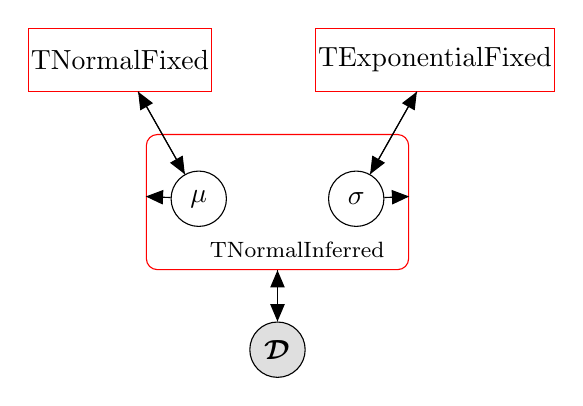
\begin{tikzpicture}[main/.style = {draw, circle, minimum size=8mm,node distance=20mm},
                    roundnode/.style={circle, fill=blue!5, minimum size=8mm},
                    squarednode/.style={rectangle, minimum size=8mm, draw=red}]]
  % nodes
  \node[obs] (D) {$\bD$};
  \node[latent, above=of D, xshift=-1cm, yshift=0.2cm] (mu) {$\mu$};
  \node[latent, above=of D, xshift=1cm, yshift=0.2cm] (sigma) {$\sigma$};
  % plates
  \node[latent, squarednode, above=of mu, xshift=-1cm] (boxOnMu) {$\mbox{TNormalFixed}$};
  \node[latent, squarednode, above=of sigma, xshift=1cm] (boxOnSigma) {$\mbox{TExponentialFixed}$};
  \plate[inner sep=0.3cm, yshift=0.15cm, color=red] {box} {(mu) (sigma)}{TNormalInferred};
  % edges
  \edge {mu} {boxOnMu};
  \edge {boxOnMu} {mu};
  \edge {sigma} {boxOnSigma};
  \edge {boxOnSigma} {sigma};
  \edge {box} {D};
  \edge {D} {box};
  \edge {mu} {box};
  \edge {sigma} {box};
\end{tikzpicture}%
 }
 \caption{Example DAG. The prior on data $\D$ is a normal distribution where the parameters $\mu$ and $\sigma$ are inferred. $\D$ is an instance of \class{TObservation}, and $\mu$ and $\sigma$ are instances of \class{TParameter}. The prior distributions on $\mu$ and $\sigma$ are fixed, since the prior parameters of these distributions can not be estimated from a single value. All existing pointers are shown with directed edges.} \label{fig:hyperpriors}
\end{figure}

In inferred prior classes, the prior parameters are pointers to \class{TParameter}. A simple example is shown in Figure \ref{fig:hyperpriors}, where a \class{TObservation} $\bD$ has a pointer to a \class{prior::TNormalInferred}. This \class{prior::TNormalInferred} has a pointer to both $\mu$ and $\sigma$, which are of type \class{TParameter}. Each prior parameter, i.e. $\mu$ and $\sigma$, has a pointer to a fixed prior distribution. In addition, each prior parameters also has a pointer to the box around them, i.e. to \class{prior::TNormalInferred}.

While in most cases a prior is solely defined on one parameter or observation $\x$, it is possible that it is defined on a vector of $P$ parameters. In such cases, we need to account for all parameters $\x_p$ when updating the prior parameters. In the following paragraphs, we will write out the likelihood ratios for the single-parameter case only. The likelihood ratio for a prior parameter $\theta$ naturally extends to
\begin{equation*}
 l_\theta = \sum_{p=1}^P \log \left(\frac{\p(\boldsymbol x_p |\theta')}{\p(\boldsymbol x_p | \theta)} \right).
\end{equation*}
for the multi-parameter case. The loop over all nodes below is hidden in \class{prior::TPriorBase} and must not be considered by the developer.

\paragraph{\class{prior::TNormalInferred}}
A normal distribution is parametrized by
\begin{itemize}
 \item mean $\mu$ (\privparam{mean}).
 \item variance $\sigma^2$ (\privparam{var}).
\end{itemize}
The log prior density and ratio are given by \eqref{eq:priorDensNormal} and \eqref{eq:priorRatioNormal}, respectively.\\
The log likelihood ratio $l_\mu$ for an update of $\mu$ is:

\begin{equation*}
 l_\mu = \log \left(\frac{\p(\boldsymbol x | \mu', \sigma^2)}{\p(\boldsymbol x | \mu, \sigma^2)} \right) = \frac{1}{2\sigma^2} \sum_{i=1}^N \left( (x_{i} - \mu)^2 - (x_{i} - \mu')^2 \right).
\end{equation*}

The log likelihood ratio $l_{\sigma^2}$ for an update of $\sigma^2$ is:

\begin{equation*}
 l_{\sigma^2} = \log \left(\frac{\p(\boldsymbol x | \mu, \sigma^{2'})}{\p(\boldsymbol x | \mu, \sigma^2)} \right) = \frac{N}{2} \log \left( \frac{\sigma^2}{\sigma^{2'}} \right)+ \frac{1}{2}\left(\frac{1}{\sigma^2} - \frac{1}{\sigma^{2'}}\right)\sum_{i=1}^N(x_{i} - \mu)^2.
\end{equation*}

For initialization of the prior parameters, we calculate the maximum likelihood estimate (MLE) $\mu$ and $\sigma^2$. The MLE $\hat\mu$ is
\begin{equation}\label{eq:MLE_mu_univariate}
 \hat \mu = \frac{1}{N} \sum_{i=1}^N x_i.
\end{equation}
If the prior is defined on a vector of $P$ parameters $\X$, the MLE $\hat\mu$ is:
\begin{equation*}
 \hat \mu = \frac{1}{\sum_{p=1}^P N_p} \sum_{p=1}^P \sum_{i=1}^{N_p} x_{p_i}.
\end{equation*}

The MLE $\hat{ \sigma^2}$ is
\begin{equation}\label{eq:MLE_var_univariate}
 \hat{ \sigma^2} = \frac{1}{N} \sum_{i=1}^N (x_i - \hat \mu)^2.
\end{equation}
If the prior is defined on a vector of $P$ parameters $\X$, the MLE $\hat{ \sigma^2}$ is:
\begin{equation*}
 \hat{ \sigma^2} = \frac{1}{\sum_{p=1}^P N_p} \sum_{p=1}^P \sum_{i=1}^{N_p} (x_{p_i} - \hat \mu)^2.
\end{equation*}

\paragraph{\class{prior::TExponentialInferred}}
An exponential distribution is parametrized by
\begin{itemize}
 \item rate $\lambda$ (\privparam{lambda}).
\end{itemize}
The log prior density and ratio are given by \eqref{eq:priorDensExponential} and \eqref{eq:priorRatioExponential}, respectively.

The log likelihood ratio $l_\lambda$ for an update of $\lambda$ is:
\begin{equation*}
 l_\lambda = \log \left(\frac{\p(\boldsymbol x | \lambda')}{\p(\boldsymbol x | \lambda)} \right) = N \log \left(\frac{\lambda'}{\lambda}\right) + (\lambda - \lambda') \sum_{i=1}^N x_i.
\end{equation*}

For the initialization of the prior parameters, we calculate the MLE for $\hat \lambda$:
\begin{equation*}
 \hat \lambda = \frac{N}{\sum_{i=1}^N x_i} ,
\end{equation*}
If the prior is defined on a vector of parameters, the MLE is:
\begin{equation*}
 \hat \lambda = \frac{\sum_{p=1}^P N_p}{\sum_{p=1}^P \sum_{i=1}^{N_p} x_{p_i}}.
\end{equation*}

\paragraph{\class{prior::TPoissonInferred}}
An Poisson distribution is parametrized by
\begin{itemize}
 \item rate $\lambda$ (\privparam{lambda}).
\end{itemize}

The log prior density and ratio are given by \eqref{eq:priorDensPoisson} and \eqref{eq:priorRatioPoisson}, respectively.

The log likelihood ratio $l_\lambda$ for an update of $\lambda$ is:
\begin{equation*}
 l_\lambda = \log \left(\frac{\p(\boldsymbol x | \lambda')}{\p(\boldsymbol x | \lambda)} \right) = \log \left(\frac{\lambda'}{\lambda}\right) \sum_{i=1}^N x_i + (\lambda - \lambda') N.
\end{equation*}

For the initialization of the prior parameters, we calculate the MLE for $\hat \lambda$:
\begin{equation*}
 \hat \lambda = \frac{\sum_{i=1}^N x_i}{N},
\end{equation*}
If the prior is defined on a vector of parameters, the MLE is:
\begin{equation*}
 \hat \lambda = \frac{\sum_{p=1}^P \sum_{i=1}^{N_p} x_{p_i}}{\sum_{p=1}^P N_p}.
\end{equation*}

\paragraph{\class{prior::TBetaInferred}}
A beta distribution is parametrized by
\begin{itemize}
 \item shape $\alpha$ (\privparam{alpha}).
 \item shape $\beta$ (\privparam{beta}).
\end{itemize}
The log prior density and ratio are given by \eqref{eq:priorDensBeta} and \eqref{eq:priorRatioBeta}, respectively.\\
The log likelihood ratio $l_\alpha$ for an update of $\alpha$ is
\begin{equation*}
 l_\alpha = \log \left(\frac{\p(\boldsymbol x | \alpha', \beta)}{\p(\boldsymbol x | \alpha, \beta)} \right) = N \left( \ln \Gamma (\alpha' + \beta) - \ln \Gamma(\alpha+\beta) + \ln \Gamma(\alpha) - \ln \Gamma(\alpha') \right) +  (\alpha' - \alpha) \sum_{i=1}^N \log x_i.
\end{equation*}

The log likelihood ratio $l_\beta$ for an update of $\beta$ is

\begin{equation*}
 l_\beta = \log \left(\frac{\p(\boldsymbol x | \alpha, \beta')}{\p(\boldsymbol x | \alpha, \beta)} \right) = N \left( \ln \Gamma (\alpha + \beta') - \ln \Gamma(\alpha+\beta) + \ln \Gamma(\beta) - \ln \Gamma(\beta') \right) +  (\beta' - \beta) \sum_{i=1}^N \log (1 - x_i).
\end{equation*}

For the initialization of the prior parameters, we calculate the method of moments estimates for $\alpha$ and $\beta$, since the MLE does not have a closed form. These estimates rely on the mean $\mu$ and variance $\sigma^2$ of $\x$:
\begin{eqnarray*}
 \mu &=& \frac{1}{N} \sum_{i=1}^N x_i, \\
 \sigma^2 &=& \frac{1}{N} \sum_{i=1}^N (x_i - \mu)^2.
\end{eqnarray*}

Let us define
\begin{equation*}
 \nu = \hat \alpha + \hat \beta = \frac{\mu(1-\mu)}{\sigma^2} -1, \text{ where } \nu > 0,\text{ therefore: } \sigma^2 < \mu(1-\mu).
\end{equation*}
The method of moments estimates for $\hat\alpha$ and $\hat\beta$ then are:
\begin{eqnarray*}
\hat \alpha &=& \mu \nu, \\
\hat \beta &=& (1 - \mu) \nu.
\end{eqnarray*}

This naturally extends to the case where the prior is defined on a vector of parameters, as the only difference is the equation for $\mu$ and $\sigma^2$:
\begin{eqnarray*}
 \mu &=& \frac{1}{\sum_{p=1}^P N_p} \sum_{p=1}^P \sum_{i=1}^{N_p} x_{p_i}, \\
 \sigma^2 &=& \frac{1}{\sum_{p=1}^P N_p} \sum_{p=1}^P \sum_{i=1}^{N_p} (x_{p_i} - \mu)^2.
\end{eqnarray*}


\paragraph{\class{prior::TGammaInferred}}
A gamma distribution is parametrized by:
\begin{itemize}
 \item shape $\alpha$ (\privparam{alpha}).
 \item rate $\beta$ (\privparam{beta}).
\end{itemize}

The log prior density and ratio are given by \eqref{eq:priorDensGamma} and \eqref{eq:priorRatioGamma}, respectively.

The log likelihood ratio $l_\alpha$ for an update of $\alpha$ is:
\begin{equation*}
 l_\alpha = \log \left(\frac{\p(\boldsymbol x | \alpha', \beta)}{\p(\boldsymbol x | \alpha, \beta)} \right) = N \left(\log \beta(\alpha' - \alpha) + \log \Gamma(\alpha) - \log \Gamma(\alpha')\right) + (\alpha'-\alpha) \sum_{i=1}^{N} \log x_i.
\end{equation*}

The log likelihood ratio $l_\beta$ for an update of $\beta$ is:
\begin{equation*}
 l_\beta = \log \left(\frac{\p(\boldsymbol x | \alpha, \beta')}{\p(\boldsymbol x | \alpha, \beta)} \right) = N \alpha \log \left( \frac{\beta'}{\beta} \right) + (\beta - \beta') \sum_{i=1}^{N} x_i.
\end{equation*}

There is no closed-form solution for the MLE of $\alpha$ and $\beta$. Instead, we use mixed type log-moment estimators that have a closed-form and are derived from the likelihood of the generalized gamma distribution.

Let us denote by $s = N \sum_{i=1}^N x_i \log x_i - \sum_{i=1}^N \log x_i \sum_{i=1}^N x_i$.
The estimate for $\alpha$ is:
\begin{equation*}
 \hat \alpha = \frac{N \sum_{i=1}^N x_i}{s},
\end{equation*}
If the prior is defined on a vector of parameters, the estimate is:
\begin{equation*}
 \hat \alpha = \frac{\sum_{p=1}^P N_p \sum_{i=1}^{N_p} x_i}{\sum_{p=1}^P s_p},
\end{equation*}

The estimate for $\beta$ is:
\begin{equation*}
 \hat \beta = \frac{N^2}{s},
\end{equation*}
If the prior is defined on a vector of parameters, the estimate is:
\begin{equation*}
 \hat \beta = \frac{\sum_{p=1}^P N_p^2}{\sum_{p=1}^P s_p}.
\end{equation*}

\paragraph{\class{prior::TBinomialInferred}}
A Binomial distribution is parametrized by
\begin{itemize}
 \item the success probability for each trial, $p$ (\privparam{p}).
\end{itemize}
The data this prior is defined on must be 2-dimensional, where the number of columns (i.e. the second dimension) is of length two, corresponding to $n_i$ and $k_i$ of the binomial distribution.

The log prior density and ratio are given by \eqref{eq:priorDensBinomial} and \eqref{eq:priorRatioBinomial}, respectively.

The log likelihood ratio $l_p$ for an update of $p$ is:
\begin{equation*}
 l_p = \log \left(\frac{\p(\boldsymbol k | \boldsymbol n, p')}{\p(\boldsymbol k | \boldsymbol n, p)} \right) = \log\left(\frac{p'}{p} \right) \sum_{i=1}^N k_i + \log\left(\frac{1-p'}{1-p} \right) \sum_{i=1}^N \left(n_i - k_i \right).
\end{equation*}
For the initialization of the prior parameters, we calculate the MLE for $p$ with
\begin{equation*}
 \hat{p} = \frac{\sum_{i=1}^N k_i}{\sum_{i=1}^N n_i}.
\end{equation*}
If the prior is defined on a vector of parameters, this gets:
\begin{equation*}
 \hat{p} = \frac{\sum_{p=1}^P \sum_{i=1}^{N_p} x_{p_i}}{\sum_{p=1}^P \sum_{i=1}^N n_{pi}}.
\end{equation*}

\paragraph{\class{prior::TNegativeBinomialInferred}}
A negative binomial distribution is parametrized by
\begin{itemize}
 \item the success probability for each trial, $p$ (\privparam{p}).
\end{itemize}
The same conditions apply to the data as in the fixed prior, see above.

The log prior density and ratio are given by \eqref{eq:priorDensNegBinomial} and \eqref{eq:priorRatioNegBinomial}, respectively.

The log likelihood ratio $l_p$ for an update of $p$ is:
\begin{equation*}
 l_p = \log \left(\frac{\p(\boldsymbol x | \boldsymbol n, p')}{\p(\boldsymbol x | \boldsymbol n, p)} \right) = \log\left(\frac{p'}{p} \right) \sum_{i=1}^N n_i + \log\left(\frac{1-p'}{1-p} \right) \sum_{i=1}^N x_i.
\end{equation*}
For the initialization of the prior parameters, we calculate the MLE for $p$ with
\begin{equation*}
 \hat{p} = \frac{\sum_{i=1}^N n_i}{\sum_{i=1}^N( n_i + x_i)}.
\end{equation*}
If the prior is defined on a vector of parameters, this gets:
\begin{equation*}
 \hat{p} = \frac{\sum_{p=1}^P \sum_{i=1}^{N_p} n_{pi}}{\sum_{p=1}^P \sum_{i=1}^N (n_{pi} + x_{pi})}.
\end{equation*}

\paragraph{\class{prior::TBernoulliInferred}}
A Bernoulli distribution is parametrized by
\begin{itemize}
 \item a probability $\pi$ (\privparam{pi}).
\end{itemize}
The log prior density and ratio are given by \eqref{eq:priorDensBernoulli} and \eqref{eq:priorRatioBernoulli}, respectively.

The log likelihood ratio $l_\pi$ for an update of $\pi$ is:
\begin{equation*}
 l_\pi = \log \left(\frac{\p(\boldsymbol x | \pi')}{\p(\boldsymbol x | \pi)} \right) = \log\left(\frac{\pi'}{\pi} \right) \sum_{i=1}^N x_i + \log\left(\frac{1-\pi'}{1-\pi} \right) \sum_{i=1}^N (1-x_i).
\end{equation*}
For the initialization of the prior parameters, we calculate the MLE for $\pi$ with
\begin{equation*}
 \hat{\pi} = \frac{\sum_{i=1}^N x_i}{N}.
\end{equation*}
If the prior is defined on a vector of parameters, this gets:
\begin{equation*}
 \hat{\pi} = \frac{\sum_{p=1}^P \sum_{i=1}^{N_p} x_{p_i}}{\sum_{p=1}^P N_p}.
\end{equation*}

\paragraph{\class{prior::TGibbsBetaBernoulliInferred}}
If the likelihood is given by a Bernoulli distribution as
\begin{equation*}
   \p(x|\pi) = \pi^x (1-\pi)^{1-x},
\end{equation*}
and the prior is given by a Beta distribution as
\begin{equation*}
   \p(\pi|\alpha, \beta) = \pi^{\alpha-1}(1-\pi)^{\beta-1}\frac{1}{\Beta(\alpha, \beta)},
\end{equation*}
then it is possible to sample directly from the posterior $\p(\pi|x)$, since the Bernoulli and the Beta distribution are conjugate. The posterior is proportional to
\begin{equation*}
   \p(\pi|x) \propto \pi^{ k + \alpha - 1}(1-\pi)^{N - k + \beta - 1},
\end{equation*}
where $k = \sum_{i=1}^N x_i$ denotes the number of successes. This is again a Beta-distribution, such that
\begin{equation*}
   \p(\pi|x) \sim \Beta(k + \alpha, N - k + \beta).
\end{equation*}
In such cases, the parameter $\pi$ does not need to be updated with the Metropolis-Hastings algorithm, but can be instead directly sampled from its posterior distribution. This is more efficient, since every update is accepted (compared to accepting only roughly $30\%$ of all updates in Metropolis-Hastings).

This prior inherits from \class{prior::TBernoulliInferred} and overrides solely the methods that update $\pi$: Instead of updating $\pi$ in Metropolis-Hastings, the function \pubfunc{doGibbs} samples from the posterior. Because it needs to know $\alpha$ and $\beta$ from the prior on $\pi$, the class additionally expects a pointer to the $\class{prior::TBetaFixed}$ prior on $\pi$.

\paragraph{\class{prior::TCategoricalInferred}}\label{categorical}
A categorical distribution is a discrete probability distribution that describes the possible results of a parameter $\boldsymbol x$ that can take on one of $K$ possible categories, with the probability of each category separately specified by a probability $\pi_k$. This prior is thus parametrized by
\begin{itemize}
 \item probabilities $\bpi$ (\privparam{pis}) of size $K$.
\end{itemize}
The probabilities $\bpi$ must sum to one: $\sum_k \pi_k = 1$. The initial values are thus normalized to satisfy this condition.\\
The log prior density of a value $x_i$ is:
\begin{equation*}
 \log \p(x_i = k | \bpi) = \pi_k.
\end{equation*}
The log prior ratio is
\begin{equation*}
 \log p_x = \log \left( \frac{\p(x = j | \bpi)}{\p(x=k|\bpi)} \right) = \log \left( \frac{\pi_j}{\pi_k} \right).
\end{equation*}
The log likelihood ratio $l_{\pi_k}$ for an update of $\pi_k$ is:
\begin{equation*}
 l_{\pi_k} = \log \left(\frac{\p(\boldsymbol x | \pi_k')}{\p(\boldsymbol x | \pi_k)} \right) = \log \left( \frac{\pi_k'}{\pi_k} \right) \sum_{i=1}^N {\cal I}(x_i = k).
\end{equation*}

For the initialization of the prior parameters, we calculate the MLE for each $\hat \pi_k$:
\begin{equation*}
 \hat \pi_k = \frac{1}{N}\sum_{i=1}^N {\cal I}(x_i = k).
\end{equation*}
If the prior is defined on a vector of parameters, the MLE is:
\begin{equation*}
 \hat \pi = \frac{1}{\sum_{p=1}^P N_p}\sum_{p=1}^P \sum_{i=1}^{N_p} {\cal I}(x_{p_i} = k).
\end{equation*}

\paragraph{\class{prior::TDirichletVarInferred}}

A Dirichlet with inferred variance distribution parametrized by
\begin{itemize}
 \item a vector of $K$ concentration parameters $\tilde{\balpha}$ (fix).
 \item a variance parameter $\sigma$ (inferred).
\end{itemize}
The values of $\tilde{\balpha}$ should be given as a comma-seperated string to the function \pubfunc{setFixedPriorParameters}, whereas $\sigma$ is a pointer to \class{TParameter}. The concentration parameters that are then used for the Dirichlet distribution are given by
\begin{equation*}
 \balpha = \frac{\tilde{\balpha}}{\sigma}.
\end{equation*}

The idea of this class is that the expected value of the parameter below does not depend on $\sigma$ but only on the normalized concentration parameter:

\begin{equation*}
 \E[X_i] = \frac{\alpha_i}{\sum_{k=1}^K \alpha_k}.
\end{equation*}

However, the variance of the parameter below may vary depending on $\sigma$:

\begin{equation*}
 \Var[X_i] = \frac{a_i (1 - a_i)}{\alpha_0 + 1},
\end{equation*}

where $a_i = \frac{\alpha_i}{\alpha_0}$ and $\alpha_0 = \sum_{k=1}^K \alpha_k$. The forumlation is such that smaller values of $\sigma$ result in smaller $\Var[X_i]$.

The log prior density and ratio are given by \ref{eq:logDensDirichlet} and \ref{eq:logRatioDirichlet} as described above for \class{TDirichletFixed}.
The log likelihood ratio $l_{\sigma}$ for an update of $\sigma$ is:

\begin{equation*}
 l_{\sigma} = \log \left( \frac{\p(\x | \balpha')}{\p(\x | \balpha)} \right) = \log \text{B}(\balpha) - \log \text{B}(\balpha') + \sum_{k=1}^K (\alpha_k' - \alpha_k) \log x_k.
\end{equation*}

For the initialization of $\sigma$ prior to the MCMC, we do a line search to find the value of $\sigma$ maximizing the log-likelihood as given by equation \ref{eq:logDensDirichlet}.

\paragraph{\class{prior::THMMPrior}}
The general framework for HMMs are described in section \ref{hmm}. Here, we will describe how the HMM parameters are updated in the MCMC. The class \class{prior::THMMPrior} serves as a base class for several specific HMM priors. As the MCMC updates are very similar among all HMM priors, we will describe the general procedure here assuming that the transition probabilities are modelled using a parameter $\theta$ and that the hidden states are represented by $z_i$ with $i= 0, \ldots, N$. The distances are given by $\delta_i$.

The HMM prior is a classic example of a non-iid prior, as the prior density of one $z_i$ depends on its neighbours $z_{i-1}$ and $z_{i+1}$. The log prior density of a value $z_i$ is
\begin{equation*}
 \log \p(z_i|\boldsymbol z_{0:N}, \boldsymbol \delta_{0:N}, \theta) = \log \p(z_i|z_{i-1}, \delta_i, \theta) + \log \p(z_{i+1}|z_{i}, \delta_{i+1}, \theta).
\end{equation*}
These probabilites correspond to the transition probabilities and are given by the element $[Q(\delta_i)]_{z_{i-1}z_i}$ from the transition matrix.
Note that the log prior density breaks down to
\begin{equation*}
 \log \p(z_0|\boldsymbol z_{0:N}, \boldsymbol \delta_{0:N}, \theta) = \log \p(z_0|\theta) + \log \p(z_{1}|z_{0}, \delta_{1}, \theta),
\end{equation*}
and
\begin{equation*}
 \log \p(z_N|\boldsymbol z_{0:N}, \boldsymbol \delta_{0:N}, \theta) = \log \p(z_N|z_{N-1}, \delta_N, \theta),
\end{equation*}
for $z=0$ and $z=N$, respectively.

The log prior ratio for an update of $z_i$ is:
\begin{eqnarray*}
 \log p_{z_i} &=& \log \left( \frac{\p(z_i'|\boldsymbol z_{0:N}, \boldsymbol \delta_{0:N}, \theta)}{\p(z_i|\boldsymbol z_{0:N}, \boldsymbol \delta_{0:N}, \theta)} \right)\\
 &=& \log \left(\frac{\p(z_i'|z_{i-1}, \delta_i, \theta)}{\p(z_i|z_{i-1}, \delta_i, \theta)} \right) + \log \left( \frac{\p(z_{i+1}|z_{i}', \delta_{i+1}, \theta)}{\p(z_{i+1}|z_{i}, \delta_{i+1}, \theta)} \right),
\end{eqnarray*}
Note that the log prior ratio breaks down to
\begin{equation*}
 \log p_{z_0} = \log \left(\frac{\p(z_0'|\theta)}{\p(z_0|\theta)} \right) + \log \left( \frac{\p(z_{1}|z_{0}', \delta_{1}, \theta)}{\p(z_{1}|z_{0}, \delta_{1}, \theta)} \right),
\end{equation*}
and
\begin{equation*}
 \log p_{z_N} = \log \left( \frac{\p(z_N'|z_{N-1}, \delta_N, \theta)}{\p(z_N|z_{N-1}, \delta_N, \theta)} \right),
\end{equation*}
for $z=0$ and $z=N$, respectively.

The log likelihood ratio $l_{\theta}$ for an update of $\theta$ is
\begin{equation}\label{eq:HMMUpdate}
 l_{\theta} = \log \left(\frac{\p(\boldsymbol z_{0:N} | \boldsymbol \delta_{0:N}, \theta')}{\p(\boldsymbol z_{0:N} | \boldsymbol \delta_{0:N}, \theta)} \right) = \log \left( \frac{\p(z_0 | \theta')}{\p(z_0 | \theta)} \right) + \sum_{i=1}^{N} \log \left( \frac{\p(z_i | z_{i-1}, \delta_i, \theta')}{\p(z_i | z_{i-1}, \delta_i, \theta)} \right).
\end{equation}

For the initialization of the prior parameters, we use the Baum-Welch algorithm described in section \ref{hmm}.

\paragraph{\class{prior::THMMBoolInferred}}
The class \class{prior::THMMBoolInferred} applies for HMMs where the hidden state $z_i$ is a binary variable with $S=2$ states: 0 and 1. The transition matrix for this prior is parametrized by two parameters $\pi$ and $\gamma$, as described in section \ref{section:TransitionProbabilities}. The class inherits from \class{prior::THMMPrior}, and equation \ref{eq:HMMUpdate} is used to calculate the log likelihood ratio for an update of $\theta = \pi, \gamma$.

\paragraph{\class{prior::THMMBoolGeneratingMatrixInferred}}
The class \class{prior::THMMBoolGeneratingMatrixInferred} applies for HMMs where the hidden state $z_i$ is a binary variable with $S=2$ states: 0 and 1. The transition matrix for this prior is parametrized by two parameters $\log \Lambda_1$ and $\log \Lambda_2$, as described in section \ref{section:TransitionProbabilities}. The class inherits from \class{prior::THMMPrior}, and equation \ref{eq:HMMUpdate} is used to calculate the log likelihood ratio for an update of $\theta = \log \Lambda_1, \log \Lambda_2$.

In simulations, we noted that for large distances (i.e. when the transition probabilities approach the stationary probabilities), different combinations of $\log \Lambda_1$ and $\log \Lambda_2$ result in exactly the same transition probabilities. The likelihood surface therefore results in a ridge. We then encountered the issue that during initialization, the Nelder-Mead algorithm optimizes $\log \Lambda_1$ and $\log \Lambda_2$ along that ridge, until the values get so large that the matrix exponential has numeric inaccuracies, and odd transition probabilities result. This is an undesired behaviour. We therefore implemented the prior \class{prior::THMMBoolInferred}, which circumvents this issue with a more elegant parametrization, and recommend to use that class for HMM prior on booleans.

\paragraph{\class{prior::THMMLadderInferred}}
The class \class{prior::THMMLadderInferred} applies for HMMs where the generator matrix has a ladder-type structure that only allows for transitions between neighbouring states. The transition matrix for this prior is parametrized by two parameters $\kappa$, as described in section \ref{section:TTransitionMatrixLadder}. The class inherits from \class{prior::THMMPrior}, and equation \ref{eq:HMMUpdate} is used to calculate the log likelihood ratio for an update of $\theta = \kappa$.

\paragraph{\class{prior::THMMCombinedScaledLadderInferred}}
The class \class{prior::THMMCombinedScaledLadderInferred} implements one or more HMMs where each chain has a transition probability given by a scaled ladder-type generator matrix. The concept of decomposing a HMM on combined states into multiple chains with specific transition probabilities is described in section \ref{section:CombinedStatesHMM}. This class is templated and takes any scaled latter-type transition matrix, with or without attractor. Specifically, the template argument \template{TransitionMatrixType} can either be \type{TTransitionMatrixScaledLadder}, \type{TTransitionMatrixScaledLadderAttractorShift} or \type{TTransitionMatrixScaledLadderAttractorShift2}, which are described in section \ref{section:TransitionProbabilities}. If the transition matrix has an attractor, the attractor for each chain must be specified in the constructor. These attractors are fixed and will not be updated in the MCMC.

Apart from (optional) attractors, the transition matrix is parametrized by three parameters, $\bkappa$, $\bnu$ and $\bmu$. These parameters are vectors where the size is given by the number of chains. If a chain $c$ consists of 3 states, the parameter $\mu_c$ is superficial and is not included.
All $\bkappa$, $\bnu$ and $\bmu$ must be strictly positive. However, the parametrization of the scaled ladder only makes sense if $\bnu$ and $\bmu$ are in [0,1], since only then the middle state is more frequent than all other states. We therefore recommend to put a sparse prior on them. In the initialization with EM, we can not specify a prior, but we still want a spare solution. Therefore, we make sure $\bnu$ and $\bmu$ are in [0,1] by applying the logistic function after optimization by Nelder-Mead.

The class inherits from \class{prior::THMMPrior}, and equation \ref{eq:HMMUpdate} is used to calculate the log likelihood ratio for an update of $\theta = \bkappa, \bnu, \bmu$.

\paragraph{\class{prior::THMMCategoricalInferred}}
The class \class{prior::THMMCategoricalInferred} applies for HMMs where the transition matrix is of type \class{TTransitionMatrixCategorical}. The hidden states are categorical with a total of $D$ states. The transition matrix for this prior is parametrized by three parameters $\pi$, $\gamma$ and $\brho$, where $\brho = \rho_1, \ldots, \rho_D$ is a vector with the constraint $\sum_d \rho_d = 1$. The class inherits from \class{prior::THMMPrior}, and equation \ref{eq:HMMUpdate} is used to calculate the log likelihood ratio for an update of $\theta = \pi, \gamma, \brho$.

\paragraph{\class{prior::TTwoNormalsMixedModelInferred}}
This class implements a special form of a mixture model of $K=2$ normal distributions:
\begin{equation*}
 \p(x_i) = (1-z_i) \Phi(\mu, \sigma_0^2) + z_i \Phi(\mu, \sigma_0^2+\sigma_1^2).
\end{equation*}
Here, $z_i$ denotes an binary indicator variable representing the two models, and $\Phi(\mu, \sigma^2)$ denotes the normal density with mean $\mu$ and variance $\sigma^2$. In this parametrization, the two mixture components share a common mean $\mu$ and the variance is larger in case $z_i = 1$ than in the case $z_i = 0$.

This prior is thus parametrized by
\begin{itemize}
\item A mean (for both components), $\mu$ (\privparam{mus}).
\item A variance for the null-model, $\sigma_0^2$, and for the one-model $\sigma_1^2$ (\privparam{vars}).
\item Indicator variables $\z$ (\privparam{z}). These are linear with size $N$.
\end{itemize}

The log prior density of a value $x_i$ is:
\begin{equation}\label{eq:logPriorDensity_NormalTwoMixedModel}
\log \p(x_i|\mu, \sigma_0^2, \sigma_1^2, z_i) =
\begin{cases}
 -\frac{1}{2}\log(\sigma_0^2) - \frac{1}{2}\log(2\pi) - \frac{1}{2\sigma_0^2}(x_i - \mu)^2 \text{ if } z_i = 0, \\
  -\frac{1}{2}\log(\sigma_0^2 + \sigma_1^2) - \frac{1}{2}\log(2\pi) - \frac{1}{2 ( \sigma_0^2 + \sigma_1^2)}(x_i - \mu)^2 \text{ if } z_i = 1.
\end{cases}
\end{equation}

The log prior ratio is:
\begin{equation*}
 \log p_x = \log \left( \frac{\p(x_i'|\mu, \sigma_0^2, \sigma_1^2, z_i)}{\p(x_i|\mu, \sigma_0^2, \sigma_1^2, z_i)} \right) =
 \begin{cases}
 \frac{1}{2\sigma_0^2}\left((x_i - \mu)^2 - (x_i' - \mu)^2\right) \text{ if } z_i = 0 \\
 \frac{1}{2(\sigma_0^2+\sigma_1^2)}\left((x_i - \mu)^2 - (x_i' - \mu)^2\right) \text{ if } z_i = 1.
\end{cases}
\end{equation*}

The log likelihood ratio $l_{\mu}$ for an update of $\mu$ is
\begin{eqnarray*}
 l_{\mu} &=& \log \left(\frac{\p(\boldsymbol x | \mu', \sigma_0^2, \sigma_1^2, \boldsymbol z)}{\p(\boldsymbol x | \mu, \sigma_0^2, \sigma_1^2, \boldsymbol z)} \right)\\
 &=& \frac{1}{2\sigma_0^2} \sum_{i=1}^N (1-z_i) \left( (x_{i} - \mu)^2 - (x_{i} - \mu')^2 \right) + \frac{1}{2\left(\sigma_0^2 + \sigma_1^2\right)} \sum_{i=1}^N z_i \left( (x_{i} - \mu)^2 - (x_{i} - \mu')^2 \right).
\end{eqnarray*}

The log likelihood ratio $l_{\sigma_0^2}$ for an update of parameter $\sigma_0^2$ is
\begin{align*}
 l_{\sigma_0^2} &= \log \left(\frac{\p(\boldsymbol x | \mu, \sigma_0^{2'}, \sigma_1^2, \boldsymbol z)}{\p(\boldsymbol x | \mu, \sigma_0^2, \sigma_1^2, \boldsymbol z)} \right) \\
 &= \begin{aligned}[t]
 & \frac{1}{2}\log\left(\frac{\sigma_0^2}{\sigma_0^{2'}}\right)\sum_{i=1}^N (1-z_i) + \frac{1}{2} \log\left(\frac{\sigma_0^2+\sigma_1^2}{\sigma_0^{2'}+\sigma_1^2}\right) \sum_{i=1}^N z_i  + \\
 &          \frac{1}{2}\left(\frac{1}{\sigma_0^2} - \frac{1}{\sigma_0^{2'}}\right)\sum_{i=1}^N(1-z_i)(x_{i} - \mu)^2 + \frac{1}{2}\left(\frac{1}{\sigma_0^2+\sigma_1^2} - \frac{1}{\sigma_0^{2'}+\sigma_1^2}\right)\sum_{i=1}^N z_i(x_{i} - \mu)^2.
 \end{aligned}
\end{align*}

The log likelihood ratio $l_{\sigma_1^2}$ for an update of $\sigma_1^2$ is
\begin{eqnarray*}
 l_{\sigma_1^2} &=& \log \left(\frac{\p(\boldsymbol x | \mu, \sigma_0^2, \sigma_1^{2'}, \boldsymbol z)}{\p(\boldsymbol x | \mu, \sigma_0^2, \sigma_1^2, \boldsymbol z)} \right) \\
 &=& \frac{1}{2}\log\left(\frac{\sigma_0^2+\sigma_1^2}{\sigma_0^2+\sigma_1^{2'}}\right) \sum_{i=1}^N z_i + \frac{1}{2}\left(\frac{1}{\sigma_0^2+\sigma_1^2} - \frac{1}{\sigma_0^2+\sigma_1^{2'}}\right)\sum_{i=1}^Nz_i(x_{i} - \mu)^2.
\end{eqnarray*}

The posterior distribution of $z_i$ can be calculated analytically, because its values are limited to few discrete states. We therefore directly sample new values of $z_i$ from the posterior distribution as specified in (\ref{eq:posterior}). The likelihood for sampling a specific $z_i$ is then given by $\p(x_i | \mu, \sigma^2_{z_i})$, and the prior by $\p(z_i | \pi )$. Note that this hold regardless of the prior distribution, e.g. HMMs.

We use an Expectation-Maximization (EM) algorithm for the initialization of the prior parameters. To simplify the EM, we assume that the variance of the null model ($\sigma_0^2$) is independent of the variance of the one-model. The EM algorithm then runs exactly as described on page \pageref{pg:EM_univariate}, except for $\mu$, which is now independent of component $k$. We can therefore initialize $\mu$ with its MLE using \eqref{eq:MLE_mu_univariate}, and don't need to update it during the EM. The initialization of the EM therefore also proceeds differently:
\begin{enumerate}
    \item Calculate the overall MLE mean $\hat \mu$ and variance $\hat \sigma^2$ of all $\x$ using \eqref{eq:MLE_mu_univariate} and \eqref{eq:MLE_var_univariate}, respectively.
    \item Calculate the log density $\log \p(x_{pi}|\hat \mu, \hat \sigma^2)$ for each data point $x_{pi}$ with \eqref{eq:priorDensNormal}. Then, calculate the average log density over all parameters as $\bar{\boldsymbol d} = \frac{1}{P}\sum_{p=1}^P \log \p(x_{pi}|\hat \mu, \hat \sigma^2)$.
    \item Data points with a low density do not fit the overall variance well, because they are far away from the mean. Therefore, sort the densities $\bar{\boldsymbol d}$ in ascending order. Assign the first 10\% of the data points $\x$ with the lowest density to $z=1$ and the rest to $z=0$.
    \item Calculate the MLE variances $\hat \sigma_0^2$ and $\hat \sigma_1^2$ based on this classification.
    \item Initialize the latent variable $z_i$ to the state that maximizes the emission probabilities.
    \item Initialize $\sigma_0^2$ and $\sigma_1^2$ by re-calculating the MLE variance based on this classification.
\end{enumerate}

We have now estimated mean and variance of null- and one-model independently, ignoring the condition that the variance of the one-model must be larger than the variance of the null-model. Therefore, we now set $\hat{\sigma_0^2} = \min(\sigma_0^2, \sigma_1^2)$ and $\hat{\sigma_1^2} = \max(\sigma_0^2, \sigma_1^2) - \hat{\sigma_0^2}$, and assign $\z$ and the prior on $\z$ accordingly.

\paragraph{\class{prior::TMultivariateNormalInferred}}
This class implements a multivariate normal prior
\begin{equation*}
 \x_i \sim {\cal N}(\bmu, \bSigma),
\end{equation*}
where $\x_i$ is a $D$-dimensional vector, parametrized by a $D$-dimensional mean vector $\bmu$ and a $D$x$D$ variance-covariance matrix $\bSigma$. Since the inverse of $\bSigma$ is positive definite and symmetric, it can be parametrized with aid of the Cholesky factorization:
\begin{equation}\label{eq:MToSigma}
\bSigma^{-1}= \M \M^T,
\end{equation}
where $\M$ is the lower triangular matrix:
\begin{equation*}
\M = \frac{1}{m} \cdot \begin{pmatrix}
m_{11} & 0 &  \ldots & 0\\
m_{21} & m_{22} & \ldots & 0\\
\vdots & \vdots & \ddots & \vdots\\
m_{D1} & m_{D2} & \ldots & m_{DD}
\end{pmatrix},
\end{equation*}
for a positive scale factor $m > 0$. This factorization allows for independent updates of the elements in the matrix $\M$ while preserving the intrinsic properties of a variance-covariance matrix.
The density of the multivariate normal distribution is:
\begin{align}
\p(\x_i | \bmu, \bSigma) &= \frac{1}{\sqrt{(2\pi)^D \det\bSigma}} \exp\left(-\frac{1}{2} (\x_i-\bmu)^T \bSigma^{-1} (\x_i-\bmu) \right)\nonumber \\
&=\frac{\frac{1}{m^D}|\prod_{r = 1}^{D}m_{rr}|}{\sqrt{(2\pi)^D}} \exp\left(-\frac{1}{2m^2}\sum_{s = 1}^{D}\left(\sum_{r = s}^{D}m_{rs} (x_{ir} - \mu_r) \right)^2 \right), \label{eq:multivariateNormalDens}
\end{align}
because the determinant of $\bSigma$ is given by
\begin{equation*}
\det \bSigma = \left(\frac{1}{m^D} \prod_{r = 1}^{D} m_{rr}\right)^{-2},
\end{equation*}
and
\begin{equation*}
(\x_i-\bmu)^T \bSigma^{-1} (\x_i-\bmu) = ||\M^T (\x_i-\bmu)||^2 = \frac{1}{m^2}\sum_{s = 1}^{D}\left(\sum_{r = s}^{D}m_{rs} (x_{ir} - \mu_r) \right)^2.
\end{equation*}
New proposals of the variance-covariance matrix $\bSigma$ are obtained by proposing new elements $m_{rr}$, $m_{rs}$ and $m$. Although this is not part of this prior, commonly recommended prior distributions for these parameters are $m \sim \text{Exp}(\lambda_m)$, $m_{rr}^2 \sim \chi_{\delta_r}^2$ where $\delta_r = D + 1 - r$ and $m_{rs} \sim {\cal N}(0,1)$. With $m$ fixed and these prior distributions for $m_{rr}$ and $m_{rs}$, $\bSigma^{-1}$ is sampled from a Wishart distribution with $D$ degrees of freedom and scale $m$ \citep{Anderson2003}.\\
A multivariate normal distribution is hence parametrized by
\begin{itemize}
 \item Means $\bmu$ of size $D$ (\privparam{mus}).
 \item A scale factor $m$ of size 1 (\privparam{m}).
 \item Diagonal elements $\bmrr$ of size $D$ (\privparam{Mrr}).
 \item Off-diagonal elements $\bmrs$ of size $T$ (\privparam{Mrs}). $T$ is given by:
    \begin{equation}\label{eq:sizeofM}
    T = \frac{D(D-1)}{2}.
    \end{equation}
    From $T$, we can also calculate $D$ with:
    \begin{equation*}
    D = \frac{1+\sqrt{1+8T}}{2}.
    \end{equation*}
    To get from a coordinate $r,s$ the linear index $p$, we calculate
    \begin{equation*}
     p = \frac{r(r-1)}{2} + s.
    \end{equation*}
\end{itemize}

The parameter on which this prior is defined, $\X$, must have dimensions $N \times D$, i.e. the number of dimensions of the multivariate normal prior should be the columns of $\X$. This is beneficial for cache handling: When calculating the prior densities, we always need one row $\x_i$ from $\X$, which corresponds to one consecutive chunk of memory because we store matrices in a row-major order.\\
The multivariate normal prior is a non-iid prior, as the prior density of one $x_{id}$ depends on all $\x_i$. The log prior density of a value $x_{id}$ with parameters $\bmu$, $\M = \{m, \bmrr, \bmrs\}$ is
\begin{equation*}
\log \p(x_{id} | \bmu, \M )= -D \log m + \sum_{r=1}^D \mrr -\frac{D}{2} \log (2\pi) -\frac{1}{2m^2}\sum_{s = 1}^{D}\left(\sum_{r = s}^{D}m_{rs} (x_{ir} - \mu_r) \right)^2.
\end{equation*}

The log prior ratio is:
\begin{align*}
\log p_{x_{id}} = \log \left( \frac{\p(x_{id}' | \bmu, \M)}{\p(x_{id} | \bmu, \M)} \right) &= \frac{1}{2m^2}\sum_{s = 1}^{D}\left( \left(\sum_{r = s}^{D}m_{rs} (x_{ir} - \mu_r) \right)^2- \left(\sum_{r = s}^{D}m_{rs} (x_{ir}' - \mu_r) \right)^2 \right)\\
&= \begin{aligned}[t]
& \frac{1}{2m^2}\Bigg(\left(x_{id}^2 - x_{id}'^2 + 2\mu_d(x_{id}' - x_{id})\right) \sum_{r=1}^{d} m_{dr}^2  + \\
&   2(x_{id} - x_{id}') \sum_{s=1}^{S} m_{ds} \sum_{r=s, r \neq d}^{D} m_{rs}(x_{ir} - \mu_r) \Bigg).
 \end{aligned}
\end{align*}
where $S = \min(d,D-1)$.\\
The log likelihood ratio $l_{\mu_d}$ for an update $\mu_d$ is:
\begin{align*}
l_{\mu_d} = \log \left( \frac{\p(\X | \mu_d', \M)}{\p(\X | \mu_d, \M)} \right) &= \frac{1}{2m^2}\sum_{i=1}^N \sum_{s = 1}^{D}\left( \left(\sum_{r = s}^{D}m_{rs} (x_{ir} - \mu_r) \right)^2- \left(\sum_{r = s}^{D}m_{rs} (x_{ir} - \mu_r') \right)^2 \right)\\
&= \begin{aligned}[t]
& \frac{1}{2m^2}\Bigg(N(\mu_d^2 - \mu_d'^2) \sum_{r=1}^{d} m_{dr}^2 +
 2(\mu_d' -\mu_d) \left(\sum_{r=1}^d m_{dr}^2\right) \left(\sum_{i=1}^N x_{id}\right) + \\
&   2(\mu_d' -\mu_d) \sum_{i=1}^N \sum_{s=1}^{S} m_{ds} \sum_{r=s, r \neq d}^{D} m_{rs}(x_{ir} - \mu_r) \Bigg).
 \end{aligned}
\end{align*}

The log likelihood ratio $l_{m}$ for an update of $m$ is:
\begin{eqnarray*}
l_{m} &=& \log \left( \frac{\p(\X | \bmu, \M')}{\p(\X | \bmu, \M)} \right) \\
 &=& ND(\log m - \log m') + \frac{1}{2}\left(\frac{1}{m^2} - \frac{1}{m'^2} \right) \sum_{i=1}^N \sum_{s = 1}^{D} \left(\sum_{r = s}^{D}m_{rs} (x_{ir} - \mu_r) \right)^2.
\end{eqnarray*}

The log likelihood ratio $l_{\mrr}$ for an update of parameter $m_{rr}$ is:
\begin{align*}
l_{\mrr} &= \log \left( \frac{\p(\X | \bmu, \M')}{\p(\X | \bmu, \M)} \right) \\
 &= N(\log \mrr' - \log \mrr) + \frac{1}{2m^2}\sum_{i=1}^N \sum_{s = 1}^{D}\left( \left(\sum_{r = s}^{D}m_{rs} (x_{ir} - \mu_r) \right)^2- \left(\sum_{r = s}^{D}m_{rs}' (x_{ir} - \mu_r) \right)^2 \right)\\
 &= \begin{aligned}[t]
 & N(\log \mrr' - \log \mrr) + \frac{1}{2m^2}\Big((\mrr^2 - \mrr'^2) \sum_{i=1}^N (x_{ir} - \mu_r)^2 +\\
 & 2(\mrr - \mrr')\sum_{i=1}^N (x_{ir} - \mu_r) \sum_{d=r+1}^D m_{dr}(x_{id} - \mu_d)\Big).
 \end{aligned}
\end{align*}

The log likelihood ratio $l_{\mrs}$ for an update of parameter $m_{rs}$ is:
\begin{align*}
l_{\mrs} &= \log \left( \frac{\p(\X | \bmu, \M')}{\p(\X | \bmu, \M)} \right) \\
 &= \frac{1}{2m^2}\sum_{i=1}^N \sum_{s = 1}^{D}\left( \left(\sum_{r = s}^{D}m_{rs} (x_{ir} - \mu_r) \right)^2- \left(\sum_{r = s}^{D}m_{rs}' (x_{ir} - \mu_r) \right)^2 \right)\\
 &= \begin{aligned}[t]
 & \frac{1}{2m^2} \left( (\mrs^2 - \mrs'^2 ) \sum_{i=1}^N(x_{ir} - \mu_r)^2 + 2(\mrs - \mrs') \sum_{i=1}^N (x_{ir} - \mu_r) \sum_{d=s, d\neq r}^D m_{ds}(x_{id} - \mu_d) \right).
 \end{aligned}
\end{align*}
Note that if $D=1$, parameter $\mrs$ is non-existant and $\mrr$ is superficial and fixed to 1, such that only $m$ is estimated.

For the initialization of the prior parameters, we calculate the MLE of $\bmu$ and $\M$. The MLE for one $\hat \mu_d$ is given by:
\begin{equation}\label{eq:MLE_mu_multivariate}
 \hat \mu_d = \frac{1}{N} \sum_{i=1}^N x_{id}.
\end{equation}
If the prior is defined on a vector of $P$ parameters, the MLE is given by
\begin{equation*}
 \hat \mu_d = \frac{1}{\sum_{p=1}^P N_p} \sum_{p=1}^P \sum_{i=1}^{N_p} x_{id}^{(p)}.
\end{equation*}

The MLE for $\bSigma$ is given by:
\begin{equation}\label{eq:MLE_var_multivariate}
  \hat \bSigma = \frac{1}{N} \sum_{i=1}^{N} (\x_i - \hat \bmu)(\x_i - \hat \bmu)^T.
\end{equation}
If the prior is defined on a vector of parameters, the MLE is given by
\begin{equation*}
  \hat \bSigma = \frac{1}{\sum_{p=1}^P N_p} \sum_{p=1}^P \sum_{i=1}^{N} (\x_i^{(p)} - \hat \bmu)(\x_i^{(p)} - \hat \bmu)^T.
\end{equation*}

We can calculate $\M$ by Cholesky factorization from the inverse of $\bSigma$ with \ref{eq:MToSigma}. We then set $m=1$ and $\mrr$ and $\mrs$ to the respective elements in $\M$.

\paragraph{\class{prior::TTwoMultivariateNormalsMixedModelInferred}}
This class implements a special mixture model of $K=2$ multivariate normal distributions:
\begin{equation*}
 \p(\x_i) = (1-z_i)\Phi(\bmu, \bSigma^{(0)}) + z_i \Phi(\bmu, \bSigma^{(1)}).
\end{equation*}
Here, $z_i$ is an binary indicator variable representing the two models, and $\Phi(\bmu, \bSigma)$ denotes the multivariate normal density with a $D$-dimensional mean vector $\bmu$ and $D$x$D$ variance-covariance matrix $\bSigma$. $\x_i$ itself is a $D$-dimensional vector.
In this parametrization, the two mixture components share a common mean vector $\bmu$ and the variance-covariance matrix is larger in case $z_i = 1$ than in the case $z_i = 0$.

We achieve this with the following parametrization: The variance-covariance matrix of the null-model is factorized as for \class{prior::TMultivariateNormalInferred} by applying Cholesky factorization to $\bSigma^{(0)}$, resulting in $\M^{(0)}$, which is split into the elements $m^{(0)}$, $\bmrr^{(0)}$ and $\bmrs^{(0)}$. The density of the null-model is thus given by equation \ref{eq:multivariateNormalDens}. The variance-covariance matrix of the one-model, $\bSigma^{(1)}$, is calculated in the following way:
\begin{enumerate}
    \item Calculate
    \begin{equation}\label{eq:Cholesky}
        \bSigma^{(0)} = \left(\M^{(0)} \M^{{(0)}^T}\right)^{-1}.
    \end{equation}
    \item Do Eigendecomposition of $\bSigma^{(0)}$:
     \begin{equation}\label{eq:eigendecomposition}
         \bSigma^{(0)} = \Q \bLambda^{(0)} \Q^{-1}.
     \end{equation}
     Here, $\bLambda^{(0)}$ is a diagonal matrix whose elements are the eigenvalues of $\bSigma^{(0)}$.
     \item Multiply with $\boldsymbol \rho$ to get $\bLambda^{(1)}$, which contains the eigenvalues of $\bSigma^{(1)}$:
     \begin{equation}\label{eq:stretchWithRho}
        \bLambda^{(1)} = \bLambda^{(0)} \left( \bOne + \brho \right),
     \end{equation}
     in matrix notation:
     \begin{equation*}
      \begin{pmatrix} \lambda_{1}^{(1)} & 0 &  \ldots & 0\\
      0 & \lambda_{2}^{(1)} & \ldots & 0\\
      \vdots\\
      0 & 0 & \ldots & \lambda_{D}^{(1)}
      \end{pmatrix} =
     \begin{pmatrix} \lambda_{1}^{(0)} & 0 &  \ldots & 0\\
      0 & \lambda_{2}^{(0)} & \ldots & 0\\
      \vdots\\
      0 & 0 & \ldots & \lambda_{D}^{(0)}
      \end{pmatrix}
      \begin{pmatrix}
      1 + \rho_{1}\\
      1 + \rho_{2}\\
      \vdots\\
      1 + \rho_{D}
      \end{pmatrix}.
     \end{equation*}
     \item Now construct $\bSigma^{(1)}$:
     \begin{equation}\label{eq:getSigma1}
         \bSigma^{(1)} = \Q \bLambda^{(1)} \Q^{-1}.
     \end{equation}
     \item From this, we get $\M^{(1)}$ with \eqref{eq:MToSigma}.
     \item We split $\M^{(1)}$ into the elements $\bmrr^{(1)}$ and $\bmrs^{(1)}$, and set $m^{(1)} = 1$.
\end{enumerate}
For $\brho > 0$, the formulation ensures that the variances and covariances are larger in case $z_i = 1$ than in the case $z_i = 0$. We can think of $\bSigma^{(1)}$ as a stretched version of $\bSigma^{(0)}$, as we stretch $\bSigma^{(0)}$ in every dimension with $\rho_d$.\\
A multivariate normal mixed model with two components is parametrized by
\begin{itemize}
  \item A mean vector (for both components), $\bmu$ of size $D$ (\privparam{mus}).
  \item Null-model: A scale factor $m^{(0)}$ of size 1 (\privparam{m}).
  \item Null-model: Diagonal elements $\bmrr^{(0)}$ of size $D$ (\privparam{Mrr}).
  \item Null-model: Off-diagonal elements $\bmrs^{(0)}$ of size $T$ (\privparam{Mrs}), see \eqref{eq:sizeofM}.
  \item Indicator variables $\z$ of size $N$ (\privparam{z}).
  \item Stretching parameter $\brho$ of size $D$ (\privparam{rhos}).
\end{itemize}

The parameter on which this prior is defined, $\X$, must have dimensions $N \times D$, i.e. the number of dimensions of the multivariate normal prior should be the columns of $\X$. This is beneficial for cache handling: When calculating the prior densities, we always need one row  $\x_i$ from $\X$, which corresponds to one consecutive chunk of memory because we store matrices in a row-major order.\\
The multivariate normal distribution is a non-iid prior, as the prior density of one $x_{id}$ depends on all $\x_i$. The log prior density of a value $x_{id}$ with parameters $\bmu$, $\M^{(0)} = \{m, \bmrr^{(0)}, \bmrs^{(0)}\}$, $\M^{(1)}$ is given by \eqref{eq:logPriorDensity_MultivariateNormalMixedModel} and the log prior ratio is given by \eqref{eq:logPriorRatio_MultivariateNormalMixedModel} (with $\bmu^{(k)} = \bmu$).

The log likelihood ratio $l_{\mu_d}$ for an update of $\mu_d$ is:
\begin{align*}
l_{\mu_d} &= \log \left( \frac{\p(\X | \mu_d', \M^{(0)}, \M^{(1)}, \boldsymbol z )}{\p(\X | \mu_d, \M^{(0)}, \M^{(1)}, \boldsymbol z )} \right) \\
&= \begin{aligned}[t]
& \frac{1}{2m^{(0)2}}\sum_{i=1}^N (1- z_i) \sum_{s = 1}^{D}\left( \left(\sum_{r = s}^{D}m_{rs}^{(0)} (x_{ir} - \mu_r) \right)^2- \left(\sum_{r = s}^{D}m_{rs}^{(0)} (x_{ir} - \mu_r') \right)^2 \right) + \\
& \frac{1}{2m^{(1)2}}\sum_{i=1}^N z_i \sum_{s = 1}^{D}\left( \left(\sum_{r = s}^{D}m_{rs}^{(1)} (x_{ir} - \mu_r) \right)^2- \left(\sum_{r = s}^{D}m_{rs}^{(1)} (x_{ir} - \mu_r') \right)^2 \right)
\end{aligned}\\
&= \begin{aligned}[t]
& \sum_{k=0}^1 \Bigg( \frac{1}{2m^{(k)2}}\Bigg((\mu_d^{2} - \mu_d^{'2}) \left( \sum_{r=1}^{d} m_{dr}^{(k)2} \right) \left(\sum_{i=1}^N {\cal I}(z_i=k) \right) + \\
& 2(\mu_d' -\mu_d) \sum_{r=1}^d m_{dr}^{(k)2} \sum_{i=1}^N {\cal I}(z_i=k) x_{id} + \\
&   2(\mu_d' -\mu_d) \sum_{i=1}^N {\cal I}(z_i=k) \sum_{s=1}^{S} m_{ds}^{(k)} \sum_{r=s, r \neq d}^{D} m_{rs}^{(k)}(x_{ir} - \mu_r) \Bigg) \Bigg).
 \end{aligned}
\end{align*}
Whenever we update any $m^{(0)}$, $\mrr^{(0)}$, $\mrs^{(0)}$ and $\rho_d$, we need to re-calculate $\M_1$. It is important to realize that the entire matrix $\M_1$ changes after any such update. Hence, for each of these updates, we need to calculate
\begin{align*}
\log \Bigg( & \frac{\p(\X | \bmu, \M^{(1)'}, \boldsymbol z)}{\p(\X | \bmu, \M^{(1)}, \boldsymbol z)} \Bigg) = \\
 & \sum_{i=1}^N z_i \left(\sum_{r=1}^D \log \left( \frac{m_{rr}^{(1)'}}{m_{rr}^{(1)}} \right) + \frac{1}{2m^{(1)^2}} \sum_{s=1}^D
\left(\left(\sum_{r=s}^D m_{rs}^{(1)} (x_{ir} - \mu_r) \right)^2 - \left(\sum_{r=s}^D m_{rs}^{(1)'} (x_{ir} - \mu_r ) \right)^2 \right)\right).
\end{align*}

The log likelihood ratio $l_{m^{(0)}}$ for an update of $m^{(0)}$ is:
\begin{align*}
l_{m^{(0)}} &= \log \left( \frac{\p(\X | \bmu, \M^{(0)'}, \M^{(1)'}, \boldsymbol z )}{\p(\X | \bmu, \M^{(0)}, \M^{(1)}, \boldsymbol z )} \right) \\
 &= \begin{aligned}[t]
    & D(\log m^{(0)} - \log m^{(0)'}) \sum_{i=i}^N (1-z_i)  + \frac{1}{2}\left(\frac{1}{m^{(0)2}} - \frac{1}{m^{(0)'2}} \right) \sum_{i=1}^N (1-z_i) \sum_{s = 1}^{D} \left(\sum_{r = s}^{D}m_{rs}^{(0)} (x_{ir} - \mu_r) \right)^2 + \\
    & \log \Bigg( \frac{\p(\X | \bmu, \M^{(1)'}, \boldsymbol z)}{\p(\X | \bmu, \M^{(1)}, \boldsymbol z)} \Bigg).
\end{aligned}
\end{align*}

The log likelihood ratio $l_{\mrr^{(0)}}$ for an update of $\mrr^{(0)}$ is:
\begin{align*}
l_{\mrr^{(0)}} &= \log \left( \frac{\p(\X | \bmu, \M^{(0)'}, \M^{(1)'}, \boldsymbol z )}{\p(\X | \bmu, \M^{(0)'}, \M^{(1)'}, \boldsymbol z )} \right) \\
&= \begin{aligned}[t]
    & \sum_{i=1}^N (1-z_i) \left( \log \left(\frac{\mrr^{(0)'}}{\mrr^{(0)}}\right)  + \frac{1}{2m^{(0)2}} \sum_{s = 1}^{D}\left( \left(\sum_{d = s}^{D}m_{ds}^{(0)} (x_{id} - \mu_d) \right)^2- \left(\sum_{d = s}^{D}m_{ds}^{(0')} (x_{id} - \mu_d) \right)^2 \right) \right) + \\
    & \log \Bigg( \frac{\p(\X | \bmu, \M^{(1)'}, \boldsymbol z)}{\p(\X | \bmu, \M^{(1)}, \boldsymbol z)} \Bigg)
\end{aligned}\\
 &= \begin{aligned}[t]
 & (\log \mrr^{(0)'} - \log \mrr^{(0)}) \sum_{i=1}^N (1-z_i) + \frac{1}{2m^{(0)2}}\Big((\mrr^{(0)2} - \mrr^{(0)'2}) \sum_{i=1}^N (1-z_i) (x_{ir} - \mu_r)^2 +\\
 & 2(\mrr^{(0)} - \mrr^{(0)'})\sum_{i=1}^N(1-z_i) (x_{ir} - \mu_r) \sum_{d=r+1}^D m_{dr}^{(0)}(x_{id} - \mu_d)\Big) + \\
 & \log \Bigg( \frac{\p(\X | \bmu, \M^{(1)'}, \boldsymbol z)}{\p(\X | \bmu, \M^{(1)}, \boldsymbol z)} \Bigg).
 \end{aligned}
\end{align*}

The log likelihood ratio $l_{\mrs^{(0)}}$ for an update of $\mrs^{(0)}$ is:
\begin{align*}
l_{\mrs^{(0)}} &= \log \left( \frac{\p(\X | \bmu, \M^{(0)'}, \M^{(1)'}, \boldsymbol z )}{\p(\X | \bmu, \M^{(0)'}, \M^{(1)'}, \boldsymbol z )} \right) \\
 &= \begin{aligned}[t]
& \frac{1}{2m^{(0)2}}\sum_{i=1}^N (1-z_i) \sum_{s = 1}^{D}\left( \left(\sum_{r = s}^{D}m_{rs}^{(0)} (x_{ir} - \mu_r) \right)^2- \left(\sum_{r = s}^{D}m_{rs}^{(0)'} (x_{ir} - \mu_r) \right)^2 \right)\\
&+ \log \Bigg( \frac{\p(\X | \bmu, \M^{(1)'}, \boldsymbol z)}{\p(\X | \bmu, \M^{(1)}, \boldsymbol z)} \Bigg)\\
 \end{aligned}\\
 &= \begin{aligned}[t]
 & \frac{1}{2m^{(0)2}} \Bigg( (\mrs^{(0)2} - \mrs^{(0)'2} ) \sum_{i=1}^N(1-z_i)(x_{ir} - \mu_r)^2 + \\
 & 2(\mrs^{(0)} - \mrs^{(0)'}) \sum_{i=1}^N (1-z_i)(x_{ir} - \mu_r) \sum_{d=s, d\neq r}^D m_{ds}^{(0)}(x_{id} - \mu_d) \Bigg) + \\
 & \log \Bigg( \frac{\p(\X | \bmu, \M^{(1)'}, \boldsymbol z)}{\p(\X | \bmu, \M^{(1)}, \boldsymbol z)} \Bigg).
 \end{aligned}
\end{align*}
Note that if $D=1$, $\bmrs^{(0)}$ is non-existant and $\bmrr^{(0)}$ is superficial and fixed to 1, such that only $m$ is estimated.

The log likelihood ratio $l_{\rho_d}$ for an update of $\rho_d$ is:
\begin{align*}
l_{\rho_d} &= \log \left( \frac{\p(\X | \bmu, \M^{(0)}, \M^{(1)'}, \boldsymbol z )}{\p(\X | \bmu, \M^{(0)'}, \M^{(1)'}, \boldsymbol z )} \right) \\
 &= \log \Bigg( \frac{\p(\X | \bmu, \M^{(1)'}, \boldsymbol z)}{\p(\X | \bmu, \M^{(1)}, \boldsymbol z)} \Bigg).
\end{align*}


The posterior distribution of $z_i$ can be calculated analytically, because its values are limited to few discrete states. We therefore directly sample new values of $z_i$ from the posterior distribution as specified in (\ref{eq:posterior}). The likelihood for sampling a specific $z_i$ is then given by $\p(\x_i | \bmu, \M^{(z_i)})$, and the prior by $\p(z_i | \pi )$. Note that this hold regardless of the prior distribution, e.g. also for HMMs.

We use an EM algorithm for the initialization of the prior parameters. To simplify the EM, we assume that the covariance matrix of the null-model ($\bSigma^{(0)}$) is independent of the covariance matrix of the one-model $(\bSigma^{(1)})$. The EM algorithm then runs exactly as described on page \pageref{pg:EM_multivariate}, except for the update step of $\bmu$. Since $\bmu$ is now independent of component $k$, we can directly estimate it with its MLE and don't need to update it during the EM. The initialization of the EM therefore also proceeds differently:
\begin{enumerate}
    \item Calculate the overall MLE mean $\bmu$ and variance-covariance matrix $\bSigma$ of all $\X$ using \eqref{eq:MLE_mu_multivariate} and \eqref{eq:MLE_var_multivariate}, respectively.
    \item Calculate the log density $\log \p(\x_{pi}|\bmu, \bSigma)$ for each data vector $\x_{pi}$ for a given parameter $p$ with \eqref{eq:multivariateNormalDens}. Then, calculate the average log density over all parameters as $\bar{\boldsymbol d} = \frac{1}{P}\sum_{p=1}^P \log \p(\x_{pi}|\bmu, \bSigma)$.
    \item Data points with a low density do not fit the overall variance well. Therefore, sort the densities $\bar{\boldsymbol d}$ in ascending order. Assign the first 10\% of the data points $\bar{\X}$ with the lowest density to $z=1$ and the rest to $z=0$.
    \item Calculate the MLE variance-covariance matrices $\bSigma^{(0)}$ and $\bSigma^{(1)}$ based on this classification.
    \item Initialize the latent variable $z_i$ to the state that maximizes the emission probabilities.
    \item Initialize $\bSigma^{(0)}$ and $\bSigma^{(1)}$ by re-calculating the MLE variance-covariance matrices based on this classification.
\end{enumerate}
We have then estimated mean and variance of null- and one-model independently, ignoring the condition that the variance of the one-model must be larger than the variance of the null-model. We therefore do eigendecomposition of both $\bSigma^{(0)}$ and $\bSigma^{(1)}$ with \eqref{eq:eigendecomposition} to obtain two matrices $\bLambda^{(0)}$ and $\bLambda^{(1)}$. We compute the norm of the diagonal $||\bLambda||_2$ for both and set the $\bLambda$ that minimizes the norm to $\bLambda_0$ (and assign $\z$ and $\pi$ accordingly). Using \eqref{eq:stretchWithRho}, we now estimate $\brho$ as:
\begin{equation*}
 \brho = \frac{\bLambda^{(1)}}{\bLambda^{(0)}} - 1,
\end{equation*}
where we set all $\rho_d < 0$ to 0.0001. We then re-calculate $\bLambda^{(1)}$ with \eqref{eq:stretchWithRho}, using these $\brho$, and $\bSigma^{(1)}$ with \eqref{eq:getSigma1}.\\
This class has 2 objects of class \class{TVarCovarMatrix} (one per component) that each store four matrices: \privparam{oldM},  \privparam{M}, \privparam{oldSigma} and \privparam{Sigma}. \class{TVarCovarMatrix} then has a couple of functions implemented that allow the conversion from $\M$ to $\bSigma$ and back.

\subsubsection{Deterministic functions}

\stattools{} allows for deterministic relationships, specifically for link functions and linear models.

\paragraph{\class{TLinkFunction}}

This class allows for an arbitary invertible link function. The class is parametrized by
\begin{itemize}
 \item A parameter (\privparam{param}).
 \item A function that transforms \privparam{param} into the value of the node below (\texttt{below = \_funDown(param)}).
 \item A function that transforms the value of the node below to \privparam{param} (\texttt{param = \_funUp(below)}). This function must be the inverse of \privfunc{funDown}.
\end{itemize}

The parameter \privparam{param} is stochastic and is updated. To evaluate its likelihood ratio, however, it must ask the parameter(s) below for the likelihood ratio. The parameter(s) below are deterministic. When calculating the likelihood ratio, they first sets their values deterministically according to function \pubfunc{valueForBelow}, and then ask the box around them to calculate the likelihood ratio.

To initialize \privparam{param}, \privfunc{funUp} is called to transform the values of the parameter below to \privparam{param}.

\paragraph{\class{TExp}}

This is a common use-case of a link function:

\begin{itemize}
 \item \privfunc{funDown} corresponds to the exponential function such that \texttt{below = exp(param)}.
  \item \privfunc{funUp} corresponds to the natural logarithm such that \texttt{param = log(below)}.
\end{itemize}

This link function is very useful if a parameter should be updated in the log-space. Updating $y = \log(x)$ instead of $x$ is commonly done for strictly positive parameters $x$ to achieve better mixing. This has two reasons:
\begin{enumerate}
 \item When updating $y = \log(x)$, this naturally imposes an exponential prior with rate 1 on $x$, because $y \sim {\cal U}(-\infty, \infty)$ results in $x \sim e^{{\cal U}(-\infty, \infty)} = \text{Exp}(1)$.
 \item The proposal range scales with the actual value of $x$. For example, a jump of 1 log-unit on $y$ corresponds to a little change in $x$ if $x$ is small and to a large change in $x$ if $x$ is large.
\end{enumerate}
In this example, $y$ corresponds to \texttt{param} and $x$ corresponds to \texttt{below}. The class is called \class{TExp} since $x = e^y$ (\texttt{below = exp(param)}), and we usually define relationships in this order (below given above).

\paragraph{\class{TLog}}

This is another common use-case of a link function:

\begin{itemize}
 \item \privfunc{funDown} corresponds to the natural logarithm such that \texttt{below = log(param)}.
  \item \privfunc{funUp} corresponds to the exponential function such that \texttt{param = exp(below)}.
\end{itemize}

Note that this class should not be used when updating a parameter in the log-space, instead use \class{TExp} which does the inverse!

\paragraph{\class{TLogistic}}

This is another common use-case of a link function:

\begin{itemize}
 \item \privfunc{funDown} corresponds to the logistic function such that \texttt{below = logistic(param)}.
  \item \privfunc{funUp} corresponds to the logit function such that \texttt{param = logit(below)}.
\end{itemize}

The logistic function (also called expit) is defined as $x = \frac{1}{1 + e^{-y}}$, where $y$ corresponds to \texttt{param} and $x$ corresponds to \texttt{below}. The logit function is the inverse of the logistic function and defined as $y = \log\left(\frac{x}{1-x}\right)$.

This link function is useful when an unconstrained parameter $y \in [-\infty, \infty]$ should be transformed into a probability $x \in [0, 1]$.

\paragraph{\class{TLogit}}

This is another common use-case of a link function:

\begin{itemize}
 \item \privfunc{funDown} corresponds to the logit function such that \texttt{below = logit(param)}.
  \item \privfunc{funUp} corresponds to the logistic function such that \texttt{param = logistic(below)}.
\end{itemize}

The logit function is defined as $x = \log\left(\frac{y}{1-y}\right)$, where $y$ corresponds to \texttt{param} and $x$ corresponds to \texttt{below}. The logistic function (also called expit) is the inverse of the logit function and defined as $y = \frac{1}{1 + e^{-x}}$.

\paragraph{\class{TLinearModel}}

This class implements a general linear model of the form

\begin{equation*}
 \Y = \X\B,
\end{equation*}

where $\Y$ is a $I \times J$ matrix, $\X$ is a $I \times K$ matrix of covariates and $\B$ is a $K \times J$ matrix of regression coefficients to be estimated. The columns of $\Y$ and $\B$ represent dependent variables that share the same set of explanatory variables. This is the most general implementation. A simple linear regression represents the special case $I=1$, $J=1$ and $K=1$. A multiple linear regression represents the case $J=1$ where there is a single dependent variable.

The general model can also be written as:
\begin{equation*}
 Y_{ij} = \beta_{0j} + \beta_{1j}X_{i1} + \beta_{2j}X_{i2} + \ldots + \beta_{Kj}X_{iK} = \beta_{0j} + \sum_{k=1}^K \beta_{kj}X_{ik},
\end{equation*}

where $\beta_{0j}$ represents an optional intercept term that can be turned on and off through the boolean template argument \template{Intercept}.

The parameter to be estimated in this model is the matrix $\B$ with elements $[\B]_{kj} = \beta_{kj}$. When one $\beta_{kj}$ is updated, one column $\Y_j = Y_{1j}, \ldots, Y_{Ij}$ changes deterministically. The likelihood ratio of this update must then be evaluated on this range of values.

To estimate initial values of $\B$, we use an ordinary least squares (OLS) scheme to solve the equation $\X\B_j = \Y_j$ for each $j = 1, \ldots, J$ using the Armadillo function \pubfunc{solve}. To account for an intercept $\beta_{0j}$, we add an extra first row with 1's to $\X$ for the OLS.

\subsection{Parameter definitions}
The class \class{TObservationDefinition} is the main interface between user, developer and the library \stattools{}. Inside this class, we can set all variables that ``define'' a parameter and observation. These are:
\begin{itemize}
 \item \privparam{priorParameters}: The prior parameters, in case these are fixed numbers.
 \item \privparam{simulationFile}: The name of the file where simulated values should be written to.
\end{itemize}
There exists a derived class, \class{TParameterDefinition}, that adds extra members specific to MCMC parameters:
\begin{itemize}
 \item \privparam{isUpdated}: Whether the parameter should be updated or not.
 \item \privparam{meanVarFile}: File to write posterior mean and value to.
  \item \privparam{statePosteriorsFile}: File to write state posteriors for categorical variables to.
 \item \privparam{traceFile}: File to write traces to.
 \item \privparam{initPropKernel}: Initial jump size for proposals.
 \item \privparam{propKernelDistr}: Name of the proposal kernel distribution (e.g. normal, uniform, integer).
 \item \privparam{oneJumpSizeForAll}: Whether all parameters in an array should share the same jump size for proposing, or alternatively have all a unique jump size.
 \item \privparam{initVal}: The initial values (given as string, to enable proper templating).
\end{itemize}
These two classes offer a variety of set- and get-functions to access these variables. A couple of other member variables are used to keep track of changed made to the definition.  \\
All of the above variables have default values.

\subsection{Providing initial values}

If needed, parameters can be initialized based on fixed initial values that are provided as a string by the user. In this case, the default initialization (based on MLE and other algorithms) is deactivated.

The string of initial values can be multiple things:
\begin{itemize}
 \item A comma-separated vector of numbers. The size of this vector must match the total size of the parameter. This option is chosen if the string contains a comma.
 \item A single number. All elements of the parameter will be set to this number. This option is chosen if the string is probably a single number (i.e. contains only numerical characters).
 \item A filename, containing the initial values. This file can have five formats:
 \begin{enumerate}
 \item A trace file, as written by this framework. This option is chosen if the filename contains ``trace''. The header of the file is then parsed and all columns that start with the name of the parameter are extracted (note that the number of columns that match must be equal to the total size of the parameter). The last line (corresponding to the last iteration) of the file is used to initialize the parameter.
 \item A file containing simulated values, as written by this framework. This option is chosen if the filename contains ``simulated''. The initialization then runs exactly as for the trace file above, as simulation files have the same format as trace files, except that they only consist of one line.
 \item A file containing the posterior means and variances, as written by this framework. This option is chosen if the filename contains ``meanVar''. The header is then parsed and all relevant columns are extracted (note that the number of columns that match must be equal to the total size of the parameter). The first line (corresponding to the posterior mean) of the file is used to initialize the parameter.
 \item A file containing the state posteriors as written by this framework. This option is chosen if the filename contains ``statePosteriors''. The header is then parsed and all relevant columns are extracted. For each column, the row index with the maximum value is used to initialize the parameter, since this corresponds to the state with the highest posterior probability.
  \item A file containing only the values for the parameter (i.e. without header), where all values are in one column and the number of rows matches the total size of the parameter.
  \item A file containing only the values for the parameter (i.e. without header), where all values are in one row and the number of columns matches the total size of the parameter.
 \end{enumerate}
\end{itemize}

\subsection{Building a DAG}

When initializing our framework, we can think of this as building a DAG. Therefore, the class that assembles all observations and parameters is called \class{TDAGBuilder}. This class is available as a singleton over \class{instances::dagBuilder()}. Let's go through its functionalities in the order we use them in a program:
\begin{itemize}
 \item The constructors of \class{TParameter} and \class{TObservation} automatically add a base class pointer to \class{instances::dagBuilder()}. There is a check for unique parameter/observation names.
 \item When the MCMC starts, the function \pubfunc{buildDAG} is called. This function executes the following steps:
 \begin{itemize}
  \item First, we create an instance of class \class{TMCMCUserInterface}. The idea is that after the developer has specified this definitions, the user can come in and modify and potentially override these definitions. Specifically, we:
  \begin{enumerate}
   \item Check if a config file has been defined on the command-line. The config file has the following format: A header with an mandatory column ``name'' and optional columns ``observation'', ``priorParameters'', ``traceFile'', ``meanVarFile'', ``statePosteriorsFile'', ``simulationFile'', ``update'', ``propKernel'', and ``sharedJumpSize''. Then, one row corresponds to one definition. We parse all modifications of one parameter/observation and re-set the definitions accordingly. Some columns only make sense for parameters, but not for observations (i.e. ``traceFile'', ``meanVarFile'', ``statePosteriorsFile'', ``update'', ``propKernel'' and ``sharedJumpSize''). If a user tries to modify these for an observation, an error is thrown. Also note that the column ``observation'' is just for information. If a user attempts to change an observation to a parameter or vice versa, an error is thrown.
   \item Check if a file with initial values and initial jump sizes has been defined on the command-line. This file must have the following format: 3 columns that are name of parameter, initial value and initial jump size. One row corresponds to one parameter definition. We parse all rows and re-set the definitions accordingly. Columns can also be empty (e.g. only specify initial value, but not initial jump size). Note that in here, only parameter definitions are currently allowed. If the initial values for an observation definition are modified, an error is thrown. The reason is that the initial values file is usually a file generated by a former run of the framework, i.e. if you want to restart the MCMC at a given position. In this file, we don't write observation values, as they never change during the MCMC. This is a design choice that can easily be changed, if this is necessary in the future.
   \item Check if configs have been defined on the command-line directly. Specifically, we loop over all config-names (as above: ``priorParameters'', ``traceFile'', etc.), and check if a command-line argument matching the pattern \texttt{paramName.config} exists (e.g. \texttt{myParam.priorParameters=...}). If yes, we re-set the definition of this parameter/observation accordingly (note that this overrides specifications from the config file).
   \item Check if initial values and/or initial jump sizes have been defined on the command-line directly. Specifically, we check if a command-line argument matching the pattern \texttt{paramName} and \texttt{paramName.jumpSize} exists. If yes, we re-set the definition accordingly (note that this overrides specifications from the init-file).
  \end{enumerate}
  \item We check for a valid DAG. A valid DAG must have 1) at least 1 observation and 2) no parameter at bottom of DAG (this must be an observation). We then initialize an instance of class \class{TDAG}. To illustrate this, consider the following complicated DAG, represented in Figure \ref{fig:DAG}.
  \begin{figure*}[t]
\begin{center}
\includegraphics[width=0.6\textwidth]{Figures/DAG.png}
\end{center}
\caption{DAG of a complicated model. We have multiple observations at the bottom of the DAG. A complicated hierarchical model is defined on these observations. We have some parameters/observations that share a common prior (e.g. observations x1/x2 share a prior, and parameters a,b,c also share a prior).}
\label{fig:DAG}
\end{figure*}
Currently, we only have pointers to each parameter/observation in the DAG (note: we don't have pointers to the priors!). Parameters that belong to the same prior (e.g. b and c) must always be simulated/initialized/updated together. Imagine we would now treat each node of the DAG (i.e. each parameter and observation) independently. The problem then is that we will simulate/initialize/update shared prior parameters multiple times, which would be a waste of computational time (or even worse). For example, if we would tell first x1 to initialize its values, and then x2 to initialize its values, we would initialize b and c twice. We therefore need an unique path through a DAG, which we can follow while simulating/initializing, and which guarantees us to visit each node exactly once. To find such a path, we use the following recursive algorithm:
\begin{enumerate}
\item Create two vectors that store pointers to \class{TNodeTyped}: \texttt{final} and \texttt{tmp}.
 \item Start at first observation at the bottom of the DAG.
 \item Call function \pubfunc{constructDAG} on current observation/parameter. This function first add the this-pointer (a pointer to \class{TNodeTyped}) to \texttt{tmp}.
 \item The function then goes to the prior. The prior checks:
 \begin{enumerate}
  \item If all children (i.e. all parameters/observations that share this prior) are present in \texttt{tmp}, the prior adds the pointer to the first parameter/observation to \texttt{final}. Then, the prior will call \pubfunc{constructDAG} of all its prior parameters, i.e. repeat steps 3) and 4).
  \item Else (not all children are present in \texttt{tmp}): Do nothing. The recursion stops.
 \end{enumerate}
 \item Re-start recursion at next observation at bottom of DAG and repeat steps 3) to 5) until all observations have been visited.
\end{enumerate}
The resulting vector (\texttt{final}) is stored inside class \class{TDAG}. For Figure \ref{fig:DAG}, we obtain a vector $\{y, x_1, a, z, d, e, i, j, h\}$. Whenever we want to...
\begin{itemize}
 \item Initialize values (with MLE/EM etc.): Go from left $\to$ right through the vector (i.e. from bottom to top through DAG). Call function \pubfunc{guessInitialValues} on each element. This will re-direct to the prior, which will initialize its prior parameters.
 \item Simulate values: Go from right $\to$ left throught the vector (i.e. from top to bottom throught DAG). Call function \pubfunc{simulateUnderPrior} on each element. This will re-direct to the prior, which will fill each of child (i.e. each parameter/observation on which this prior is defined) with random values from the prior distribution.
\end{itemize}
To update parameters, we use another vector of base class pointers. This is because i) for updating, the order does not matter and ii) we do not want to update deterministic parameters. The function \pubfunc{update} will be called for each parameter present in this vector.
 \end{itemize}
 \item In the last step, the function \pubfunc{initializeStorage} is called, that will go through the DAG and initialize the dimensions, storage and dimension names of all parameters (by comparing the expectations based on the prior with the developer-defined dimensions). This function can only be executed after all observations have been filled with data, since the dimensions of some parameters depend on the dimensions of the observations that only known after reading the data.
\end{itemize}

\subsection{MCMC files}

We distinguish four types of MCMC files:
 \begin{enumerate}
  \item Trace files. During the MCMC, every \privparam{thinning}'st iteration, we write the parameter values to a trace file. The header contains the parameter name(s) (if the parameter is an array, it creates one column per element of the array). The rows are the values of this parameter per iteration.
  \item MeanVar files. These contain the posterior mean and variance of the parameter and are written at the end of the MCMC. The header contains the parameter name(s) and there are two rows: mean and variance.
  \item State posterior files. For categorical variables, these contain the posterior probability for each state, $\p(z = Z | \D)$. This corresponds to the fraction of times the parameter took this value during the MCMC.
  The names of the trace, meanVar and statePosteriors file are given by the parameter definition. If multiple parameters share the same file, they will be written as adjacent columns. Note that all parameters that share a state posterior file must have the same number of states (otherwise the number of rows in the file don't match). This is checked upon construction.
  \item State file. This file has three columns: name, value and jump size. It contains the current values and jump sizes for all parameters of a certain iteration. The idea is that this file is written every $i^{th}$ iteration (and is overwritten every time), as well as after the last iteration. It can then be used as a init-file for re-starting another MCMC exactly at the location where the old one has stopped, e.g. if the program crashed or if the MCMC has not reached convergence.
 \end{enumerate}
 Finally, we write all parameter configurations to a config-file. This file has the same format as the config-file that can be read when initializing the parameters, and can hence be used to re-start an MCMC with the same configurations as a previous MCMC.

\subsection{The MCMC}
Class \class{TMCMC} is the class that a developer needs to instantiate. A typical procedure would be:
\begin{enumerate}
 \item Read the data into a \class{TMultiDimensionalStorage} object.
 \item Create all parameters and observations, as well as their corresponding priors.
 \item Create an instance of class \class{TMCMC}. Call function \pubfunc{runMCMC}. This will first initialize all parameters with MLE/EM etc., and then run the MCMC algorithm.
\end{enumerate}
General MCMC parameters are (specified over the command line):
\begin{itemize}
 \item \privparam{iterations}: The number of iterations for the MCMC.
 \item \privparam{burnin}: The number of iterations for the burnin.
 \item \privparam{numBurnin}: The number of burnins to run.
 \item \privparam{thinningStateFile}: Write a state file every $i^{th}$ iteration. By default, no state file is written.
 \item \privparam{writeBurnin}: Write the trace after the initialization adn during the burnin, too.
 \item \privparam{thinning}: Write to the trace file every $i^{th}$ iteration.
\end{itemize}

\subsection{Simulations}
The function \pubfunc{simulate} of class \class{TSimulator} simulates values under the prior distribution (top-down in DAG), also filling observations with random values. The simulated values will be written to file specified in the definition. Note that if values should be read in specific file format for observations, the developer will again need to get the pointer to the observation and write the values himself, because the framework does not know how to handle specific file formats. Parameters will only be simulated if no initial values have been set.

\section{The EM algorithm}\label{em}

The expectation-maximization (EM) algorithm is an iterative algorithm that provides maximum-likelihood estimates of parameters in the presence of latent variables. Let us denote by $\X$ the observed data, by $\btheta$ the model parameters and by $\z$ the hidden (latent) variables. We will assume the most general model with $K$ independent observations $\X = \x^{(1)}, \ldots, \x^{(K)}$, where each $\x^{(k)} = x_1^{(k)}, \ldots, x_N^{(k)}$ is of length $N$ with $k = 1, \ldots, K$.

The EM algorithm seeks to obtain parameter estimates of $\btheta$ that maximize the marginal likelihood $\L(\btheta)$:

\begin{equation*}
 \L(\btheta) = \p(\X | \btheta) = \sum_{\z} \p(\X, \z | \btheta) = \sum_{\z} \L_c(\btheta).
\end{equation*}

Here, $\L_c(\btheta)$ denotes the complete data likelihood that treats $\z$ as observed.
The EM algorithm proceeds by iterating between two steps.
In the expectation step (E-step), the $Q$-function

\begin{equation*}
 Q(\btheta | \btheta') = \E \left[ \log \L_c(\btheta) | \X, \btheta' \right] = \sum_{\z} \log \p(\X, \z | \btheta) \p(\z | \X, \btheta')
\end{equation*}

is calculated using the current parameter estimates $\btheta'$. This can be factorized to

\begin{equation}{\label{eq:Q}}
 Q(\btheta | \btheta') = \sum_{k=1}^K \sum_{i=1}^N \sum_{z=1}^Z \log \p(x_i^{(k)}, z | \btheta)  \p(z | x_i^{(k)}, \btheta'),
\end{equation}

where $Z$ denotes the number of hidden states. The weights $\p(z | x_i^{(k)}, \btheta')$ can be calculated with the aid of Bayes' Theorem as

\begin{equation}\label{eq:EM_weights}
\p(z | x_i^{(k)}, \btheta') = \frac{\p(x_i^{(k)}, z | \btheta')}{\sum_{h=0}^Z \p(x_i^{(k)}, h |\btheta')}.
\end{equation}

In the maximization step (M-step), the values $\btheta$ that maximize the $Q$-function are determined:

\begin{equation*}
 \tilde{\btheta} = \argmax_{\btheta} Q(\btheta | \btheta'),
\end{equation*}

and these estimates $\tilde{\btheta}$ are then used as $\btheta'$ in the next EM iteration.

In many models, hierarchical parameters $\bpi \subseteq \btheta$ are used to model the distribution of the hidden states $\z$. The complete data likelihood $\L_c(\btheta)$ can then be factorized as

$$
\L_c(\btheta) = \p(\X, \z | \btheta) = \p(\X | \z, \bphi) \p(\z | \bpi),
$$


where $\bphi = \btheta_{-\bpi}$ denotes the parameter vector $\btheta$ without $\bpi$. In such cases, the $Q$-function from equation \eqref{eq:Q} can be written as

\begin{equation*}
 Q(\bphi, \bpi | \bphi', \bpi') = \sum_{k=1}^K \sum_{i=1}^N \sum_{z=1}^Z \left( \log \p(x_i^{(k)} | z, \bphi) + \log \p(z | \bpi) \right)  \p(z | x_i^{(k)}, \bphi', \bpi'),
\end{equation*}

and the corresponding EM weights $\p(z | x_i^{(k)}, \bphi', \bpi')$ can be calculated as

\begin{equation}\label{eq:EM_weights_with_prior}
\p(z | x_i^{(k)}, \bphi', \bpi') = \frac{\p(x_i^{(k)} | z, \bphi') \p(z | \bpi') }{\sum_{h=0}^Z \p(x_i^{(k)} | h, \bphi') \p(h | \bpi')}.
\end{equation}

\stattools{} partitions the EM algorithm in three main classes. Class \class{TLatentVariableWithRep} represents the observation model $\p(x_i^{(k)} | z, \bphi)$. Class \class{TEMPriorIndependent\_base} represents the distribution of the hidden states $\p(z | \bpi)$. And finally, class \class{TEM} runs the EM algorithm and coordinates the interaction between the latent variable and EM prior. In the following, these classes are described in more detail.

\subsection{\class{TLatentVariableWithRep} and \class{TLatentVariable}}\label{section:TLatentVariableWithRep}

The class \class{TLatentVariableWithRep} represents the observational model and is in charge of calculating $\p(\X, \z | \bphi)$. It is the most general representation of a latent variable model that also allows for multiple independent observations (replicates). In many applications, however, there is a single observation and the additional index $k$ is superfluous. The class \class{TLatentVariable} inherits from \class{TLatentVariableWithRep} and provides a simpler interface without the index $k$. Apart from this, both classes follow the same logic and structure. In the following, we will describe the interface of \class{TLatentVariableWithRep}, as this is the more general case, but we note that the interface of \class{TLatentVariable} is the same except that all replicate indices $k$ are omitted from the function definition.

Both classes are abstract base classes and define a single pure virtual function:

\begin{enumerate}
 \item \func{calculateEmissionProbabilities(size\_t i, size\_t k, TDataVector v)}: This function calculates the probabilities $\p(x_i^{(k)}, z | \bphi)$ at index \variable{i} and replicate \variable{k} for all possible hidden states $z = 1, \ldots, Z$ and stores these probabilities in the vector \variable{v}.
\end{enumerate}

A developer who wishes to implement the EM algorithm must therefore derive from \class{TLatentVariableWithRep} (if there are replicates) or \class{TLatentVariable} otherwise, and override the function \pubfunc{calculateEmissionProbabilities}. Both classes provides more virtual functions that may be overridden if needed. There are three main use-cases that can be combined in any way: i) run EM, ii) calculate likelihood and iii) estimate state posteriors. The functions that need to be implemented for each use-case are described in the following three sections.

\subsubsection{Run EM}
If the goal is to obtain MLE estimates of $\bphi$, the following functions should be considered for overriding. Note that it might not be necessary to override all of them, e.g. if there is no memory to be allocated for storing EM results, some functions may be omitted. We will describe these functions in the order they are called.

Before the EM starts, these two functions are called:
\begin{enumerate}
 \item \pubfunc{prepareEMParameterEstimationInitial}: Initialize temporary values or allocate memory needed to store the EM weights (only if necessary).
 \item \pubfunc{initializeEMParameters}: Estimate an initial guess of $\bphi$.
\end{enumerate}

Then, in each EM iteration, these functions are called:
\begin{enumerate}
 \item \pubfunc{prepareEMParameterEstimationOneIteration}: Called right in the beginning of the iteration. This function should reset temporary values for the new iteration (only if necessary).
 \item \func{handleEMParameterEstimationOneIteration(size\_t i, size\_t k, TDataVector v)}: The vector \variable{v} contains the EM weights $\p(z | x_i^{(k)}, \bphi', \bpi')$ that were calculated within \stattools{} according to equation \eqref{eq:EM_weights_with_prior}. Depending on the M-step, the developer will need to either store the weights or sum them up.
 \item \pubfunc{finalizeEMParameterEstimationOneIteration}: Called at the end of the iteration. This function should perform the M-step.
 \item \pubfunc{reportEMParameters}: Called at the end of the iteration. Provides the possibility to report the updated parameters $\bphi$ to the logfile.
\end{enumerate}

At the very end of the EM, this function is called:
\begin{enumerate}
 \item \pubfunc{finalizeEMParameterEstimationFinal}: Clear temporary variables or memory (only if necessary).
\end{enumerate}

\subsubsection{Calculate likelihood}

To calculate the likelihood, the following functions should be considered for overriding.

\begin{enumerate}
 \item \pubfunc{prepareLLCalculation}: Initialize temporary values or allocate memory needed to store the EM weights (only if necessary).
 \item \pubfunc{finalizeLLCalculation}: Clear temporary variables or memory (only if necessary).
\end{enumerate}

\subsubsection{Estimate state posterior probabilities}

To estimate the state posterior probabilities $\p(z | \X, \bphi, \bpi)$ for all $z=1, \ldots, Z$, the following functions should be considered for overriding.

\begin{enumerate}
 \item \pubfunc{prepareStatePosteriorEstimation}: Initialize temporary values or allocate memory needed to store the EM weights (only if necessary).
 \item \func{handleStatePosteriorEstimation(size\_t i, size\_t k, TDataVector v)}: The vector \variable{v} contains the state posterior probabilities (i.e. the EM weights) $\p(z | x_i^{(k)}, \bphi', \bpi')$ that were calculated within \stattools{} according to equation \eqref{eq:EM_weights_with_prior}. Depending on the objective, these probabilities can be stored or processed.
 \item \pubfunc{finalizeStatePosteriorEstimation}: Clear temporary variables or memory (only if necessary).
\end{enumerate}

A common use-case is to write the state posterior probabilities to a file. In such a case, the base class \class{TLatentVariableWithRep} already implements the following functions:

\begin{enumerate}
 \item \pubfunc{prepareStatePosteriorEstimationAndWriting}: Opens file and writes header.
 \item \pubfunc{handleStatePosteriorEstimationAndWriting}: Writes state posterior probabilities $\p(z | x_i^{(k)}, \bphi', \bpi')$ to file.
 \item \pubfunc{finalizeStatePosteriorEstimationAndWriting}: Clear temporary variables or memory (only if necessary).
\end{enumerate}

If necessary, these functions can be overridden by the developer to write custom files.

\subsection{\class{TEMPriorIndependent\_base}}

The class \class{TEMPriorIndependent\_base} represents the hierarchical model on the hidden states $\z$ and is in charge of calculating $\p(\z | \bpi)$. It is an abstract base class and defines a single pure virtual function:

\begin{enumerate}
 \item \func{operator(size\_t i, size\_t z)}: This function calculates the probability $\p(z_i | \bpi)$ at index \variable{i}
\end{enumerate}

A developer who whishes to implement the EM algorithm must therefore derive from \class{TEMPriorIndependent\_base} and override the function \pubfunc{operator}. The class provides more virtual functions that may be overridden if needed. If the goal is to obtain MLE estimates of $\bpi$, the following functions should be considered for overriding.

Before the EM starts, the following functions are called:
\begin{enumerate}
 \item \pubfunc{prepareEMParameterEstimationInitial}: Initialize temporary values or allocate memory needed to store the EM weights (only if necessary).
 \item \pubfunc{initializeEMParameters}: Estimate an initial guess of $\bpi$. By default, the initial guess is obtained by one full loop over all $\X$, calculating the maximum likelihood state $\hat{z}$ for each index $i$ and calling \pubfunc{handleEMParameterInitialization} with this state.
 \item \func{handleEMParameterInitialization(size\_t i, size\_t z)}: Store or sum the guess of the hidden state \variable{z}.
 \item \pubfunc{finalizeEMParameterInitialization}: Get an initial guess for $\bpi$ based on the guesses of the hidden states $\z$ obtained by the previous function.
\end{enumerate}

Then, in each EM iteration, these functions are called:
\begin{enumerate}
 \item \pubfunc{prepareEMParameterEstimationOneIteration}: Called right in the beginning of the iteration. This function should reset temporary values for the new iteration (only if necessary).
 \item \func{handleEMParameterEstimationOneIteration(size\_t i, TDataVector v)}: The vector \variable{v} contains the EM weights $\p(z | x_i^{(k)}, \bphi', \bpi')$ that were calculated within \stattools{} according to equation \eqref{eq:EM_weights_with_prior}. Depending on the M-step, the developer will need to either store the weights or sum them up.
 \item \pubfunc{finalizeEMParameterEstimationOneIteration}: Called at the end of the iteration. This function should perform the M-step.
 \item \pubfunc{reportEMParameters}: Called at the end of the iteration. Provides the possibility to report the updated parameters $\bphi$ to the logfile.
\end{enumerate}

At the very end of the EM, this function is called:
\begin{enumerate}
 \item \pubfunc{finalizeEMParameterEstimationFinal}: Clear temporary variables or memory (only if necessary).
\end{enumerate}

A typical EM prior is the categorical distribution, as described in section \ref{categorical}. The prior \class{prior::TCategoricalInferred} inherits from \class{TEMPriorIndependent\_base} and and can be readily used for any latent variable model where $z | \bpi \sim \mbox{Categorical}(\bpi)$.

\subsection{\class{TEM}}\label{section:TEM}

Class \class{TEM} runs the EM algorithm and the coordinates the interaction between classes \class{TLatentVariableWithRep} and \class{TEMPriorIndependent\_base}. In line with the use-cases described before, it provides three main functionalities:

\begin{enumerate}
 \item \pubfunc{runEM}: Run the EM algorithm to find the ML estimates of $\bphi$ and $\bpi$.
 \item \pubfunc{calculateLL}: Calculate the marginal likelihood $\L(\bphi, \bpi)$ given fixed estimates $\bphi$ and $\bpi$.
 \item \pubfunc{estimateStatePosteriors}: Estimate the state posterior probabilities $\p(z | \X, \bphi, \bpi)$ for all states $z=1, \ldots, Z$ given fixed estimates $\bphi$ and $\bpi$. If called with a filename, the state posterior probabilities will automatically be written to a file.
\end{enumerate}

The EM algorithm will iterate until i) the difference in log-likelihoods between two iterations is smaller than some threshold (default $10^{-4}$) or until ii) the maximum number of iterations is reached.

\subsubsection{SQUAREM}

The EM algorithm is very stable and guarantees a monotonic increase of the likelihood. However, the EM algorithm is also infamous for its slow, linear convergence, which can result in very long run times, especially for high-dimensional problems. Multiple acceleration schemes have been proposed. \stattools{} implements the SQUAREM method \citep{varadhan2008}, which provides an off-the-shelf solution applicable to any model. The SQUAREM algorithm in \stattools{} is adapted from \citep{varadhan2008, du2020}, and one SQUAREM cycle runs as described in algorithm \ref{algo:SQUAREM}. The SQUAREM cycles are repeated until convergence or when a maximum number of iterations is reached. The SQUAREM is implemented within \class{TEM} and is called through the function \pubfunc{runSQUAREM}.

It is well possible that the SQUAREM proposes non-valid parameter values (e.g. negative values for parameters that need to be positive). It therefore rejects all updates that result in invalid parameters.

The SQUAREM algorithm requires direct access to get and set the EM parameters in both latent variable and EM prior. If a SQUAREM is used, both the latent variable and EM prior class must override the following functions:

\begin{itemize}
 \item \pubfunc{getParameters}: Return the current values of all EM parameters $\btheta$.
 \item \func{setParameters(coretools::TConstView<PrecisionType> Params)}: Set all EM parameters $\btheta$ according to values given in \texttt{Params}. Must return \texttt{true} if these parameters are valid, and \texttt{false} otherwise.
\end{itemize}

If the SQUAREM is used, but these functions are not implemented, an error is thrown.

\begin{algorithm}[t]
\caption{One SQUAREM cycle}\label{algo:SQUAREM}
\begin{algorithmic}
\State $\btheta_1 \gets \mbox{EMupdate}(\btheta_0)$
\If{converged}
  \State stop
\EndIf
\State $\btheta_2 \gets \mbox{EMupdate}(\btheta_1)$
\If{converged}
  \State stop
\EndIf
\State $L_{\btheta_2} \gets \mbox{CalculateLL}(\btheta_2)$
\State $\r = \btheta_1 - \btheta_0$
\State $\v = (\btheta_2 - \btheta_1) - \r$
\State $\alpha = -\frac{||\r||}{||\v||}$
\State $\btheta_{sq} = \btheta_0 - 2 \alpha \r + \alpha^2 \v$
\If{$\btheta_{sq}$ is not valid}
  \State $\btheta_0 \gets \btheta_2$
  \State continue to next iteration
\EndIf
\State $L_{\btheta_{sq}} \gets \mbox{CalculateLL}(\btheta_{sq})$
\If{$L_{\btheta_{sq}} > L_{\btheta_2}$}
  \State $\btheta_0 \gets \mbox{EMupdate}(\btheta_{sq})$
\Else
  \State  $\btheta_0 \gets \btheta_2$
\EndIf
\State continue to next iteration
\end{algorithmic}
\end{algorithm}

\section{Hidden Markov Models}\label{hmm}
A Hidden Markov Model (HMM) assumes that a hidden, underlying Markov model emits noisy observations. The states $\z = (z_0, \ldots, z_N)$ of the Markov model can thus not be observed directly, but only inferred through the data $\x = (x_0, \ldots, x_N)$. We will assume that the hidden states are discrete and denote by $Z$ the number of hidden states such that $z_i \in 1, \ldots, Z$ for all $i = 1, \ldots, N$.

A HMM is characterized by three probabilities: the transition probabilities, the initial state probability and the emission probabilities. In the following sections, I will describe those probabilities and how they are modelled within \stattools{}.

\subsection{Transition probabilities}\label{section:TransitionProbabilities}
The transition probabilities $\p(z_i|z_{i-1})$ model the Markov assumption of the hidden states. Transition probabilities can be organized into a transition matrix $\Q$ whose element $[\Q]_{jk}$ represents the probability of moving from state $j$ to state $k$. The transition probabilities may be either parametrized directly or through a transition rate matrix.
A transition rate matrix $\bLambda$ is an infinitesimal generator of a transition matrix and is defined such that the rows sum to zero, $[\bLambda]_{jj} = -\sum_{k\neq j} [\bLambda]_{jk}$, while $[\bLambda]_{jk} \geq 0$ for $j \neq k$. The transition matrix is then given by the matrix exponential of the transition rate matrix, $\Q = e^{\bLambda}$ \citep{suhov2008}. However, it generally makes sense to assume that the transition probabilities are affected by the distance $\delta_i$ between two neighbouring observations $i$ and $i-1$. A classic example is the distance between two genetic markers (in space) or the distance between two recordings (in time). We therefore define $\Q(\delta_i)$ for a distance $\delta_i$ as
 \begin{equation*}
  \Q(\delta_i) = e^{\delta_i \bLambda}.
 \end{equation*}

Since the number of possible distances is large and the computation of the transition probabilities for a specific distance expensive, we group the distances $\delta_i$ into $E+1$ ensembles such that
\begin{equation}\label{eq:distGroups}
 e_i = \lceil \log_2 \delta_i + 1 \rceil - 1 , e_i = 0,\ldots,E,
\end{equation}
for every data point $i$. By using the $\log_2$-transformation, the bin size scales with the distance: all points with distance 1 go in the first group, all points with distance 2-3 into the second, all points with distance 4-7 in the third etc. This is implemented in class \class{genometools::TDistancesBinned}.

We then use the same transition matrix $\Q(2^e)$ for all data points in ensemble $e$. We thus only need to calculate the transition matrix for the first ensemble $e=0$ where $\Q(2^0) = \Q(1)$, which corresponds to the transition matrix for a distance of $\delta = 1$. The transition matrices for all other ensembles can then be obtained through the recursion $\Q(e) = \Q{(e - 1)}^2$, which is relatively cheap to calculate.

In the following sections, we will describe the transition matrices that are implemented in \stattools{}.

\subsubsection{\class{TTransitionMatrixBool}}\label{section:TTransitionMatrixBool}
This transition matrix generalizes the concept of a Bernoulli prior to a Markov chain by defining two parameters:
\begin{itemize}
 \item $\pi$: The stationary probability for $z=1$. This is equivalent to the success probability of the Bernoulli prior.
 \item $\gamma$: Modulates the expected peak width, i.e. the amount of clustering.
\end{itemize}

Our transition matrix is:
\begin{equation*}
 \Q =  \frac{1}{1+\gamma} \begin{pmatrix}
  1-\pi+\gamma & \pi \\
  1-\pi & \pi + \gamma
\end{pmatrix} .
\end{equation*}

The stationary probability then is exactly $\pi$:
\begin{equation*}
\frac{\pi}{\pi + 1-\pi} = \pi.
\end{equation*}

The parameter $\gamma$ modulates the expected peak width. For $\gamma = 0$, the transition matrix is:
\begin{equation*}
 \Q = \begin{pmatrix}
  1-\pi & \pi \\
  1-\pi & \pi
\end{pmatrix} .
\end{equation*}
meaning that the probability to be in a specific state $z_i$ is completely independent of the previous state $z_{i-1}$: this corresponds to a ``memory-less'' Bernoulli process.
For any $\gamma > 0$, the expected peak width increases relative to the peak width under a Bernoulli process. In fact, the expected peak length is given by

\begin{equation*}
 \E(\mbox{peak width}) = \frac{1}{Q_{1\to0}} = \frac{1+\gamma}{1-\pi},
\end{equation*}
where the peak width under the Bernoulli model is simply $\frac{1}{1-\pi}$.

\subsubsection{\class{TTransitionMatrixCategorical}}\label{section:TTransitionMatrixCategorical}
This transition matrix generalizes the concept of a categorical prior to a Markov chain by defining three parameters:
\begin{itemize}
 \item $\pi$: The stationary probability for $z \neq 0$.
 \item $\gamma$: Modulates the expected peak width, i.e. the amount of clustering.
 \item $\brho = (\rho_1, \ldots, \rho_Z)$: Model the probability to jump into a certain state $z$.
\end{itemize}

Our goal is to define a transition matrix of form

\begin{equation*}
 \Q = \begin{pmatrix}
  1 - \sum_{z=1}^Z \lambda_z & \lambda_1 & \lambda_2 & \ldots & \lambda_Z \\
  \lambda_0 & 1 - \lambda_0 & 0 & \ldots & 0 \\
  \lambda_0 & 0 & 1 - \lambda_0 & \ldots & 0 \\
  \vdots & \vdots & \vdots & \ddots & \vdots \\
  \lambda_0 & 0 & 0 & \ldots & 1 - \lambda_0
\end{pmatrix} .
\end{equation*}

as a function of parameters $\pi$, $\gamma$ and $\rho$. The stationary distribution of this transition matrix can be derived from the following system of linear equations:

\begin{equation*}
 \p_0 = \left( 1 - \sum_{z=1}^Z \lambda_z \right) \p_0 + \lambda_0 \sum_{z=1}^Z \p_z
 \end{equation*}
and
 \begin{equation*}
 \p_0 + \sum_{z=1}^Z \p_z = 1,
\end{equation*}

which results in

\begin{equation}\label{eq:la0pi}
 \pi = \sum_{z=1}^Z \p_z = \frac{\sum_{z=1}^Z \lambda_z}{\lambda_0 + \sum_{z=1}^Z \lambda_z}.
\end{equation}

We have thus defined $\pi$ as the stationary distribution to be in a non-zero state.

We note that the expected peak width for this transition matrix is:
\begin{equation*}
 \E(\mbox{peak width}) = \frac{1}{Z} \sum_{z=1}^Z \frac{1}{Q_{z \to 0}} = \frac{1}{\lambda_0},
\end{equation*}

whereas the expected peak width for a Bernoulli process is $\frac{1}{1-\pi}$. We now parametrize our transition matrix such that the peak width corresponds to the Bernoulli process if $\gamma = 0$, but results in more clustering if $\gamma > 0$:

\begin{equation*}
 \E(\mbox{peak width}) = \frac{1 + \gamma}{1 - \pi}.
\end{equation*}

Solving for $\lambda_0$ results in
\begin{equation*}
 \lambda_0 = \frac{1 - \pi}{1 + \gamma}.
\end{equation*}

With these equations at hand, we readily define $\sum_{z=1}^Z \lambda_z$ as:

\begin{equation*}
 \sum_{z=1}^Z \lambda_z = \frac{\pi}{1 + \gamma}.
\end{equation*}

So far, our parametrization acts on all $\lambda_z$ jointly, as we defined $\pi$ and $\gamma$ on $\sum_{z=1}^Z \lambda_z$. In addition, we now want the model the probability to jump into a certain state $z$ by a parameter $\rho_z$ such that

\begin{equation*}
 \lambda_z = \frac{\rho_z \pi}{1 + \gamma},
\end{equation*}

where we have the constraint that $\sum_{z=1}^Z \rho_z = 1$.

Our transition matrix then is:
\begin{equation*}
 \Q =  \frac{1}{1 + \gamma} \begin{pmatrix}
  1 + \gamma - \pi & \rho_1 \pi & \rho_2 \pi & \ldots & \rho_Z \pi \\
  (1-\pi) & \gamma + \pi & 0 & \ldots & 0 \\
    (1-\pi) & 0 & \gamma + \pi & \ldots & 0 \\
  \vdots & \vdots & \vdots & \ddots & \vdots \\
  (1-\pi) & 0 & 0 & \ldots & \gamma + \pi
\end{pmatrix}.
\end{equation*}

\subsubsection{\class{TTransitionMatrixBoolGeneratingMatrix}}\label{section:TTransitionMatrixBoolGeneratingMatrix}

This transition matrix is defined through a $2 \times 2$ transition rate matrix $\bLambda$, which is parametrized by $\lambda_1$ and $\lambda_2$:
\begin{equation}\label{eq:generatorMatrixBool}
 \bLambda =   \begin{pmatrix}
  -\lambda_1 & \lambda_1 \\
  \lambda_2 & -\lambda_2
\end{pmatrix} .
\end{equation}
The stationary probabilities are calculated with
\begin{equation*}
\p(z_0 = 0 | \lambda_1, \lambda_2) = \frac{\lambda_2}{\lambda_1 + \lambda_2}
\end{equation*}
and
\begin{equation*}
\p(z_0 = 1 | \lambda_1, \lambda_2) = 1 - \p(z_0 = 0| \lambda_1, \lambda_2).
\end{equation*}

This transition rate matrix is implemented in the class \class{TGeneratingMatrixBool}. As described above, the transition matrix for a distance $\delta = 1$ is given by the matrix exponential of the generating matrix.

\subsubsection{\class{TTransitionMatrixLadder}}\label{section:TTransitionMatrixLadder}
This transition matrix is defined through a $Z \times Z$ ladder-type transition rate matrix $\bLambda$, which is parametrized by $\kappa$:
    \begin{equation*}
    \bLambda = \kappa \cdot \left(\begin{array}{cccccc}
    -1 & 1 & 0 & \dots & 0 & 0\\
    1 & -2 & 1 & \dots & 0 & 0\\
    \vdots & \vdots & \vdots & \ddots & \vdots & \vdots\\
    0 & 0 & 0 & \dots & 1& -1\\
    \end{array}\right).
    \end{equation*}
The stationary probabilities are simply $\frac{1}{Z}$ for each state.

This transition rate matrix is implemented in the class \class{TGeneratingMatrixLadder}. As described above, the transition matrix for a distance $\delta = 1$ is given by the matrix exponential of the generating matrix.

\subsubsection{\class{TTransitionMatrixScaledLadder}}\label{section:TTransitionMatrixScaledLadder}
This transition matrix is defined through a $Z \times Z$ ladder-type transition rate matrix $\bLambda$ with an attractor state, which is parametrized by $\kappa$, $\nu$ and $\mu$ \citep{Galimberti2020}:

\begin{equation*}
    \bLambda = \kappa \cdot \left(\begin{array}{ccccccccc}
    -1 & 1 & 0 & 0 & \dots & 0 & 0 & 0 & 0\\
    \mu & -1-\mu & 1 & 0 & \dots & 0 & 0 & 0 & 0\\
     0  & \mu & -1-\mu & 1 & \dots & 0 & 0 & 0 & 0\\
    \vdots & \vdots & \vdots & \vdots & \ddots & \vdots & \vdots & \vdots & \vdots\\
    0 & 0 & 0 & 0 & \dots & 1 & -1-\mu & \mu & 0\\
    0 & 0 & 0 & 0 & \dots & 0 & 1 & -1-\mu & \mu\\
    0 & 0 & 0 & 0 & \dots & 0 & 0 & 1 & -1
    \end{array}\right),
\end{equation*}

where the middle row of this matrix (the attractor) is given by
\begin{equation*}
    (\begin{array}{ccccccccc}
     0  & \ldots & 0 & \nu\mu & -2 \nu\mu & \nu\mu & 0 & \ldots & 0)\\
\end{array}.
\end{equation*}
The parameter $\mu$ models the rate of moving towards the peripheral states of the matrix. If $\mu \approx 1$, it is equally likely up or down, whereas if $\mu \approx 0$, it is very unlikely to move towards the periphery of the matrix. The parameter $\nu$ models the rate of leaving the attractor. If $\nu \approx 1$, it is likely to leave the attractor, whereas if $\nu \approx 0$, it is very unlikely to leave the attractor.

The stationary distribution for this Markov Chain can be calculated directly from the parameters of the generator matrix as:
\begin{equation*}
  \Pi = c \cdot \left(\begin{array}{cccccccccccc}
  1  & \frac{1}{\mu} & \frac{1}{\mu^2} & \ldots & \frac{1}{\mu^{T-1}} & \frac{1}{\mu^T\nu} & \frac{1}{\mu^{T-1}} & \ldots & \frac{1}{\mu^2} & \frac{1}{\mu} & 1
\end{array}\right),
\end{equation*}
where
\begin{equation*}
  c = \frac{(\mu-1)\nu\mu^{T}}{2\nu\mu(\mu^{T}-1)+\mu-1}.
\end{equation*}

Here, $T = \frac{Z-1}{2} $ denotes the number of states on one side of the attractor state, where we enforce that $Z$ is an odd number.

If $\mu = 1$, this equation results in a division by zero. For this case, we use the following equation to calculate the stationary:
\begin{equation*}
  \Pi = c \cdot \left(\begin{array}{cccccccccccc}
  \nu  & \nu & \nu & \ldots & \nu & 1 & \nu & \ldots & \nu & \nu & \nu
\end{array}\right),
\end{equation*}
where
\begin{equation*}
  c = \frac{1}{Z\nu - \nu + 1}.
\end{equation*}

$\kappa$, $\mu$ and $\nu$ all must be strictly positive. However, only if $\mu$ and $\nu$ are in (0,1], the attractor state is actually attracting. We therefore constrain $\mu$ and $\nu$ to [0,1] by running optimization in the logistic space.

This transition rate matrix is implemented in the class \class{TGeneratingMatrixScaledLadder}. As described above, the transition matrix for a distance $\delta = 1$ is given by the matrix exponential of the generating matrix.

\subsubsection{\class{TTransitionMatrixScaledLadderAttractorShift}}
This transition matrix is defined through a $Z \times Z$ ladder-type transition rate matrix $\bLambda$ with an attractor state, which is parametrized by $\kappa$, $\nu$ and $\mu$. This parametrization is exactly equivalent to the previous one (\class{TGeneratingMatrixScaledLadder}) with the only difference that the attractor row does not need to be in the middle row. There is thus an extra parameter $ix$ that corresponds to the row index of the attractor (0 corresponding to the top row, 1 to the second row etc).

If there are only two states, the transition rate matrix $\bLambda$ is given by:
    \begin{equation*}
    \bLambda = \begin{cases}
    \kappa \cdot  \left(\begin{array}{cc}
    -\nu & \nu \\
    1 & -1
    \end{array}\right)  & \mbox{if } ix = 0 \vspace{0.2cm}\\

    \kappa \cdot  \left(\begin{array}{cc}
    -1 & 1 \\
    \nu & -\nu
    \end{array}\right) & \mbox{if } ix = 1.
    \end{cases}
    \end{equation*}

Note that in this case, there is no $\mu$, since the matrix would be over-parametrized.

If there are three states, the transition rate matrix $\bLambda$ is given by:
    \begin{equation*}
    \bLambda = \begin{cases}
    \kappa \cdot  \left(\begin{array}{ccc}
    -\nu\mu & \nu\mu & 0 \\
    1 & -1-\mu & \mu \\
    0 & 1 & -1
    \end{array}\right)  & \mbox{if } ix = 0 \vspace{0.2cm}\\
    \kappa \cdot  \left(\begin{array}{ccc}
    -1 & 1 & 0 \\
    \nu & -2\nu & \nu \\
    0 & 1 & -1
    \end{array}\right)  & \mbox{if } ix = 1 \vspace{0.2cm}\\
    \kappa \cdot  \left(\begin{array}{ccc}
    -1 & 1 & 0 \\
    \mu & -1-\mu & 1 \\
    0 & \nu\mu & -\nu\mu
    \end{array}\right) & \mbox{if } ix = 2.
    \end{cases}
    \end{equation*}
Note that in the case of three states and $ix$=1, there is no $\mu$ since also here, $\mu$ and $\nu$ are non-identifiable.

The stationary is complicated to calculate explicitly. We instead solve a system of normal equations, as explained in section \ref{section:InitialStateDistr}.


This transition rate matrix is implemented in the class \class{TGeneratingMatrixScaledLadderAttractorShift}. As described above, the transition matrix for a distance $\delta = 1$ is given by the matrix exponential of the generating matrix.

\subsubsection{\class{TTransitionMatrixScaledLadderAttractorShift2}}

This transition matrix is defined through a $Z\times Z$ ladder-type transition rate matrix $\bLambda$ with an attractor state, which is parametrized by $\kappa$, $\nu$ and $\mu$ as well as a index $ix$ that corresponds to the row index of the attractor (0 corresponding to the top row, 1 to the second row etc.). This parametrization is similar to the previous one (\class{TGeneratingMatrixScaledLadderAttractorShift}), with the exception that the attractor row is parametrized only by $\nu$ (without $\mu$) to improve convergence.

The transition rate matrix $\bLambda$ is given by:
\begin{equation*}
    \bLambda = \kappa \cdot \left(\begin{array}{ccccccccc}
    -1 & 1 & 0 & 0 & \dots & 0 & 0 & 0 & 0\\
    1-\mu & -2 & 1+\mu & 0 & \dots & 0 & 0 & 0 & 0\\
     0  & 1-\mu & -2 & 1+\mu & \dots & 0 & 0 & 0 & 0\\
    \vdots & \vdots & \vdots & \vdots & \ddots & \vdots & \vdots & \vdots & \vdots\\
    0 & 0 & 0 & 0 & \dots & 1+\mu & -2 & 1-\mu & 0\\
    0 & 0 & 0 & 0 & \dots & 0 & 1+\mu & -2 & 1-\mu\\
    0 & 0 & 0 & 0 & \dots & 0 & 0 & 1 & -1
    \end{array}\right),
    \end{equation*}

where the attractor row is
    \begin{equation*}
    (\begin{array}{ccccccccc}
     0  & \ldots & 0 & \nu & -2\nu & \nu & 0 & \ldots & 0)\\
    \end{array}.
    \end{equation*}

The parameter $\mu$ models the rate of moving away from the periphery towards the attractor. If $\mu \approx 0$, it's equally likely to move up or down. If $\mu \approx 1$, it is much more likely to move towards the attractor.
The parameter $\nu$ models the rate of leaving the attractor. If $\nu \approx 0$, it's very unlikely to leave the attractor. If $\nu \approx 1$, it becomes more and more likely to leave the attractor.

If there are only two states, the transition rate matrix $\bLambda$ is given by:
    \begin{equation*}
    \bLambda = \begin{cases}
    \kappa \cdot  \left(\begin{array}{cc}
    -\nu & \nu \\
    1 & -1
    \end{array}\right)  & \mbox{if } ix = 0 \vspace{0.2cm}\\

    \kappa \cdot  \left(\begin{array}{cc}
    -1 & 1 \\
    \nu & -\nu
    \end{array}\right) & \mbox{if } ix = 1.
    \end{cases}
    \end{equation*}

Note that in this case, there is no $\mu$, since the matrix would be over-parametrized.

If there are three states, the transition rate matrix $\bLambda$ is given by:
    \begin{equation*}
    \bLambda = \begin{cases}
    \kappa \cdot  \left(\begin{array}{ccc}
    -\nu & \nu & 0 \\
    1+\mu & -2 & 1-\mu \\
    0 & 1 & -1
    \end{array}\right)  & \mbox{if } ix = 0 \vspace{0.2cm}\\
    \kappa \cdot  \left(\begin{array}{ccc}
    -1 & 1 & 0 \\
    \nu & -2\nu & \nu \\
    0 & 1 & -1
    \end{array}\right)  & \mbox{if } ix = 1 \vspace{0.2cm}\\
    \kappa \cdot  \left(\begin{array}{ccc}
    -1 & 1 & 0 \\
    1-\mu & -2 & 1+\mu \\
    0 & \nu & -\nu
    \end{array}\right) & \mbox{if } ix = 2.
    \end{cases}
    \end{equation*}
Note that in the case of three states and $ix$=1, there is no $\mu$.

The stationary is complicated to calculate explicitly. We instead solve a system of normal equations, as explained in section \ref{section:InitialStateDistr}.


This transition rate matrix is implemented in the class \class{TGeneratingMatrixScaledLadderAttractorShift2}. As described above, the transition matrix for a distance $\delta = 1$ is given by the matrix exponential of the generating matrix.

\subsection{Initial state distribution}\label{section:InitialStateDistr}
The initial state distribution $\p(z_0)$ models the distribution of the first hidden state $z_0$. It often makes sense to assume that the initial state distribution follows the stationary distribution of the Markov chain, which is given by the transition matrix $\Q$.
Depending on the parametrization of $\Q$, the stationary distribution may be calculated explicitly, as it is the case for the transition matrices described in sections \ref{section:TTransitionMatrixBool}, \ref{section:TTransitionMatrixCategorical}, \ref{section:TTransitionMatrixBoolGeneratingMatrix}, \ref{section:TTransitionMatrixLadder} and \ref{section:TTransitionMatrixScaledLadder}.

If this is not possible, the stationary distribution can be calculated from the transition matrix $\Q$ using normal equations as follows. We are attempting to find a solution for
\begin{equation*}
 \bpi = \bpi \Q,
\end{equation*}
such that
\begin{equation*}
 \sum_{z=1}^Z \pi_z = 1.
\end{equation*}
We can re-arrange the above expressions to
\begin{eqnarray*}
 \bpi - \bpi \Q &=& \boldsymbol 0 \\
 \bpi(\I - \Q) &=& \boldsymbol 0.
\end{eqnarray*}
We can add the constraint that all $\bpi$ must sum to one by adding an extra column of 1's to $(\I - \Q)$ and an extra 1 to the zero vector (call this new vector $\boldsymbol b$). To simplify the notation, we will write $\bpi$ as a column vector and hence transpose $\I - \Q$ (call this new matrix $\A$):
\begin{equation*}
 \begin{pmatrix}
  1-Q_{11} & -Q_{21} & \dots & -Q_{Z1} \\
  -Q_{12} & 1-Q_{22} & \dots & -Q_{Z2} \\
  \vdots & \vdots & \ddots & \vdots \\
  -Q_{1Z} & -Q_{2Z} & \dots & 1-Q_{ZZ} \\
  1 & 1 & \ldots & 1
\end{pmatrix}
\begin{pmatrix}
  \pi_1\\
  \pi_2\\
  \vdots\\
  \pi_Z
 \end{pmatrix}
 =
 \begin{pmatrix}
 0\\
 0\\
 \vdots\\
 0\\
 1
 \end{pmatrix}
\end{equation*}
We now solve $\A \bpi = \boldsymbol b$, which is overdetermined, and can be solved with the normal equation
\begin{equation*}
 \A^T \A \bpi=\A^T \boldsymbol b.
\end{equation*}

This is achieved using the matrix library Armadillo \citep{sanderson2016, sanderson2019}.

\subsection{Emission probabilities}
The emission probabilities $\p(x_i^{(k)} | z_i)$ represent the observational model. In fact, the emission probabilities by themselves are ``ignorant'' of the Markov assumption of the hidden states $\z$ and as such not different from any other latent variable model. In \stattools{}, they are simply latent variables deriving from the class \class{TLatentVariableWithRep}, as described in  \ref{section:TLatentVariableWithRep}, regardless if the latent variable has a Markov property or not.

\subsection{The forward-backward algorithm}

Given the transition probabilities $\p(z_i | z_{i-1})$ , the initial state probability $\p(z_0)$ and the emission probabilities $\p(x_i | z_i)$, we can define the joint distribution of the HMM as

\begin{equation*}
 \p(\z, \x) = \p(z_0) \prod_{i=1}^N \p(z_i | z_{i-1}) \prod_{i=0}^N \p(x_i | z_i) .
\end{equation*}

Note that this is easily extendable to multiple $K$ independent observations. For simpler notation, we will omit the index $x^{(k)}$ in the following equations.

A major goal is to estimate $\p(z_i | \x)$ for all data points $i$, which is the state posterior probability of the hidden state $z_i$ given all the data $\x$. This can be calculated efficiently with the forward-backward algorithm, which relies on the fact that by conditioning on the state $z_i$ at index $i$, we can break the chain into two parts, the past and the future. This allows us to factorize the joint distribution to

\begin{equation*}
\p(z_i, \x_{0:N}) = \p(z_i, \x_{0:i}) \p(\x_{i+1:N} | z_i):= \alpha_i(z_i)\beta_i(z_i).
\end{equation*}

Here, $\alpha_i(z_i):=\p(z_i, \x_{0:i})$ is the probability to observe the past data up index $i$ and to be in state $z_i$, and $\beta_i(z_i):= \p(\x_{i+1:N} | z_i)$ is the probability of all future data given that the hidden state at index $i$ is $z_i$.
The state posterior probability $\p(z_i | \x_{0:N})$ is then given by:

\begin{equation}\label{eq:f_b_gamma}
\p(z_i | \x_{0:N}) = \frac{\alpha_i(z_i)\beta_i(z_i)}{\sum_{z_i}\alpha_i(z_i)\beta_i(z_i)}.
\end{equation}

This state posterior probability is commonly denoted by $\gamma_i(z_i) = \p(z_i | \x_{0:N})$. In \stattools{}, this equation in implemented in class \class{THMMPosteriorGamma}.

Both $\alpha_i(z_i)$ and $\beta_i(z_i)$ can be calculated efficiently with recursions.

\subsubsection{The forward recursion}

The forward probabilities $\alpha_i(z_i)$ can be calculated efficiently by starting with $\alpha_0(z_0) = \p(x_0 | z_0) \p(z_0)$ and then propagating to the index on the right where $\alpha_i(z_i)$ is given by

\begin{equation*}
\alpha_i(z_i) = \p(x_i | z_i) \sum_{z_{i-1}=1}^Z \p(z_i | z_{i-1}) \alpha_{i-1}(z_{i-1}).
\end{equation*}

Since these probabilities can get very small, we normalize them at each step:

\begin{equation*}
\p(z_i| \x_{0:i})= \displaystyle \frac{\alpha_i(z_i)}{\sum_{z_i}\alpha_i(z_i)}.
\end{equation*}

The forward recursion is implemented in the \stattools{} class \class{THMMForwardAlpha}.

\subsubsection{The backward recursion}

The backward probabilities $\beta_i(z_i)$ can be calculated efficiently by starting at $\beta(z_N)=1$ and then propagating to the index on the left where $\beta_i(z_i)$ is given by
\begin{equation*}
\beta_i(z_i) = \sum_{z_{i+1}=1}^Z \p(z_{i+1} | z_i) \p(x_{i+1} |z_{i+1}) \beta(z_{i+1}),
\end{equation*}

As above, we normalize the probabilities at each step.

The backward recursion is implemented in the \stattools{} class \class{THMMBackwardBeta}.

\subsection{The Baum-Welch algorithm}

The Baum-Welch algorithm is a special case of the expectation-maximization (EM) algorithm used for maximum likelihood estimation in HMMs. The following description of the Baum-Welch algorithm is mostly based on \citet{Wegmann2019}. Using the same notation as in section \ref{em}, we denote by $\X$ the observed data, by $\btheta$ the model parameters and by $\z$ the hidden (latent) variables. We will assume the most general model with $K$ independent observations $\X = \x^{(1)}, \ldots, \x^{(K)}$, where each $\x^{(k)} = x_0^{(k)}, \ldots, x_N^{(k)}$ is of length $N$ with $k = 1, \ldots, K$.

The model parameters $\btheta$ govern all initial distributions $\p(z_0)$, the transition probabilities $\p(z_i | z_{i-1})$ and the emission probabilities $\p(x_i^{(k)} | z_i)$. The complete data log likelihood is given by
\begin{equation*}
 \l_c(\btheta) = \sum_{k=1}^K \left[ \log \p(z_0^{(k)}) + \sum_{i=1}^N \log \p(z_i^{(k)} | z_{i-1}^{(k)}) + \sum_{i=0}^N \log \p(x_i^{(k)} | z_i^{(k)}) \right].
\end{equation*}

Maximum likelihood estimates of $\btheta$ can be obtained by iteratively maximizing the $Q$-function $Q(\btheta | \btheta')=\E[\l_c(\btheta)|\btheta', \X]$, which is defined as

\begin{eqnarray*}
Q(\btheta | \btheta') &=& \sum_{k=1}^K \E\left[\log \p(z_0^{(k)}) | \x_{0:N}^{(k)}, \btheta'\right] + \sum_{k=1}^K \sum_{i=1}^N \E\left[\log \p(z_i^{(k)} | z_{i-1}^{(k)}) | \x_{0:N}^{(k)}, \btheta'\right] + \ldots\\
&& + \sum_{k=1}^K \sum_{i=0}^N \E\left[\log \p(x_i^{(k)} | z_i^{(k)}) | \btheta'\right]\\
&=& \sum_{k=1}^K \sum_{z_0}\gamma_0^{(k)}(z_0)\log\p(z_0)  + \sum_{k=1}^K \sum_{i=1}^N \sum_{z_i}\sum_{z_{i-1}}\xi_i^{(k)}(z_i, z_{i-1})\log\p(z_i | z_{i-1})  + \ldots\\
&& + \sum_{k=1}^K \sum_{i=0}^N\sum_{z_i}\gamma_i^{(k)}(z_i)\log \p(x_i^{(k)} | z_i),
\end{eqnarray*}
where the $\gamma_i^{(k)}(z_i)$ and $\xi_i^{(k)}(z_i, z_{i-1})$ denote the expectation weights $\p(z_i|\x_{0:N}^{(k)})$ and $\p(z_i, z_{i-1}| \x_{0:N}^{(k)})$, respectively. These weights can be calculated efficiently with the forward-backward algorithm, where the $\gamma_i^{(k)}(z_i)$ are given by

\begin{equation*}
\gamma_i^{(k)}(z_i) = \frac{\alpha_i^{(k)}(z_i)\beta_i^{(k)}(z_i)}{\sum_{h}\alpha_i^{(k)}(h)\beta_i^{(k)}(h)}.
\end{equation*}

and all $\xi_i^{(k)}(z_i , z_{i-1})$ by
\begin{equation}\label{eq:xi_baum_welch}
\xi_i^{(k)}(z_i , z_{i-1}) := \p(z_i, z_{i-1}| \x_{0:N}^{(k)})  \propto \alpha_{i-1}^{(k)}(z_{i-1}) \p(z_i | z_{i-1}) \beta_i^{(k)}(z_i) \p(x_i^{(k)} | z_i),
\end{equation}
where one has to normalize such that the sum over $z_i$ adds up to one. In \stattools{}, this is implemented in class \class{THMMPosteriorXi}.


In line with the EM algorithm, \stattools{} partitions the Baum-Welch algorithm in three main classes. Class \class{TLatentVariableWithRep} represents the observation model $\p(x_i^{(k)} | z_i)$ and is exactly the same as in the EM framework. Class \class{TTransitionMatrix\_baseWithRep} represents the transition probabilities $\p(z_{i} | z_{i-1})$. And finally, class \class{THMM} runs the forward-backward and/or the Baum-Welch algorithm and coordinates the interaction between the latent variable and transition matrix. In the following, the latter two classes are described in more detail.

\subsection{\class{TTransitionMatrix\_base}}

The class \class{TTransitionMatrix\_base} represents the transition probabilities and is in charge of calculating $\p(z_i | z_{i-1})$. It is an abstract base classes and defines two pure virtual functions:

\begin{enumerate}
 \item \func{operator(size\_t i, size\_t from, size\_t to)}: This function calculates the transition probability $\p(z = \mbox{to} | z = \mbox{from})$ at data point \variable{i}.

 \item \func{stationary(size\_t z)}: This function calculates the stationary probability $\p(z)$.
\end{enumerate}

The class has a pre-defined implementation of initial probabilities, which are simply estimated as the expected number of the $K$ independent runs that started in state $z_0$:

$$
\p(z_0) = \frac{1}{K} \sum_{k=1}^K \gamma_0^{(k)}(z_0).
$$

We will assume that this implementation will be used in all applications, and won't describe the functions needed to override this default below for simplicity. However, we note that every function listed below that is applicable to \variable{TransitionProbabilities} can also be defined for \variable{InitialDistribution} (e.g. \pubfunc{handleEMParameterEstimationOneIterationTransitionProbabilities} and \pubfunc{handleEMParameterEstimationOneIterationInitialDistribution}), and can be easily overridden if needed.

A developer who whishes to implement an HMM must derive from \class{TTransitionMatrix\_base} and override the functions \pubfunc{operator} and \pubfunc{stationary}. The class class provides more virtual functions that may be overridden if needed. If the goal is to run a Baum-Welch algorithm, the following functions should be considered for overriding.

Before the EM starts, the following functions are called:
\begin{enumerate}
 \item \pubfunc{prepareEMParameterEstimationInitial}: Initialize temporary values or allocate memory needed to store the EM weights (only if necessary).
 \item \pubfunc{initializeEMParameters}: Estimate an initial guess of the transition matrix parameters. By default, the initial guess is obtained by one full loop over all $\X$, calculating the maximum likelihood state $\hat{z}$ for each index $i$ and calling  \pubfunc{handleEMParameterInitializationTransitionProbabilities} with this state.
 \item  \func{handleEMParameterInitializationTransitionProbabilities(size\_t i, size\_t from, size\_t to)}: Store or sum the guess of the hidden state \variable{from} to hidden state \variable{to}.
 \item \pubfunc{finalizeEMParameterInitializationTransitionProbabilities}: Get an initial guess for the transition matrix parameters based on the guesses of the hidden states $\z$ obtained by the previous function.
\end{enumerate}

Then, in each EM iteration, these functions are called:
\begin{enumerate}
 \item \pubfunc{prepareEMParameterEstimationOneIterationTransitionProbabilities}: Called right in the beginning of the iteration. This function should reset temporary values for the new iteration (only if necessary).
 \item \func{handleEMParameterEstimationOneIterationTransitionProbabilities(size\_t i, THMMPosteriorXi Xi)}: The object \variable{Xi} contains the EM weights $\xi_i^{(k)}(z_i , z_{i-1})$ that were calculated within \stattools{} according to equation \eqref{eq:xi_baum_welch}. Depending on the M-step, the developer will need to either store the weights or sum them up.
 \item \pubfunc{finalizeEMParameterEstimationOneIterationTransitionProbabilities}: Called at the end of the iteration. This function should perform the M-step.
 \item \pubfunc{reportEMParameters}: Called at the end of the iteration. Provides the possibility to report the updated parameters to the logfile.
\end{enumerate}

At the very end of the EM, this function is called:
\begin{enumerate}
 \item \pubfunc{finalizeEMParameterEstimationFinal}: Clear temporary variables or memory (only if necessary).
\end{enumerate}

In addition, the class \class{TTransitionMatrix\_base} provides functions to simulate hidden states based on the transition matrix:

\begin{enumerate}
 \item \func{simulateStates(Container Data)}: Fills a (templated) container with hidden states according to the transition probabilities. Iteratively calls the function \pubfunc{sampleNextState}.
 \item \func{sampleNextState(size\_t i, size\_t from}: Samples the next state given the previous state \variable{from} according to the transition probabilities.
\end{enumerate}

\subsubsection{\class{TTransitionMatrixDistances}}

As described in section \ref{section:TransitionProbabilities}, \stattools{} implements a collection of transition matrices that are scaled with the distance between two neighbouring data points. The class \class{TTransitionMatrixDistances} inherits from \class{TTransitionMatrix\_base} and overrides all virtual functions described above such that the parameters of any arbitrarily parametrized transition matrix can be estimated.

The most important member variables of \class{TTransitionMatrixHMMDistancesBase} are:
\begin{itemize}
 \item \privparam{distances}: A pointer an instance of class \class{TDistancesBinnedBase} that handles the distances $\delta_i$ between adjacent data points. As described in section  \ref{section:TransitionProbabilities}, these distances are binned to $E$ ensembles for computational reasons.

 \item \privparam{tau\_allDist}: A vector of size $E+1$ that stores the current transition matrices ($\Q(0), \Q(1), \ldots, \Q(E)$) as \armadillo{} matrices. Here, $\Q(0)$ represents the stationary distribution $\p(z_0)$, and all subsequent $\Q(e)$ represent the transition matrices for ensemble $e$.

 \item \privparam{tau\_allDist\_old}: A vector of size $E+1$ of \armadillo{} matrices. If used within an MCMC, these correspond to the old transition matrices. If used within an Baum-Welch, these store the EM sums $\xi$.

 \item \privparam{optimizer}: A pointer to a derived class of \class{TTransitionMatrixDistancesOptimizerBase}, which handles the optimization of the transition matrix parameters in the M-step.
\end{itemize}

The following virtual functions of class \class{TTransitionMatrix\_base} are overridden:

\begin{enumerate}
\item \func{operator(size\_t i, size\_t from, size\_t to)}: This function returns the transition probability $\p(z = \mbox{to} | z = \mbox{from})$ at data point \variable{i}, which is stored in \privparam{tau\_allDist[e]} for ensemble \variable{e} of index \variable{i}.

\item \func{stationary(size\_t z)}: This function returns the stationary probability $\p(z)$, which is stored in \privparam{tau\_allDist[0]}.
\item \pubfunc{initializeEMParameters}: Three initialization types are supported (enum \enum{TypeTransMatInitialization}). \enum{none} implies no initialization and keeps the user-provided values. \enum{ML} implies maximum-likelihood estimation through \pubfunc{handleEMParameterInitializationTransitionProbabilities}. \enum{defaultValues} implies that the default values of the transition matrix parameters are used, which are defined in the corresponding transition matrix class.
\item \func{handleEMParameterInitializationTransitionProbabilities(size\_t i, size\_t from, size\_t to)}: This sums up all the transitions \variable{from} $\to$ \variable{to} for all data points that fall within the same ensemble $e$.
\item \pubfunc{finalizeEMParameterEstimationOneIterationTransitionProbabilities}: If initialization type is \enum{ML}, this will call the function \pubfunc{finalizeEMParameterEstimationOneIterationTransitionProbabilities}, which is also used at the end of a regular EM iteration.
\item \pubfunc{prepareEMParameterEstimationOneIterationTransitionProbabilities}: This fills \privparam{tau\_allDist\_old} with zeros.
 \item \func{handleEMParameterEstimationOneIterationTransitionProbabilities(size\_t i, THMMPosteriorXi Xi)}: This sums up all \variable{Xi} for all data points that fall within the same ensemble $e$.
 \pubfunc{finalizeEMParameterEstimationOneIterationTransitionProbabilities}: This class asks the \privparam{optimizer} to maximize the $Q$-function.
\end{enumerate}

In addition, the class provides functions to simulate distances (\pubfunc{simulateDistances}) and to simulate hidden states according to the transition matrix parameters and distances (\pubfunc{sampleNextState}). Also, it is possible to activate the reporting of EM parameters to the logfile through the function \pubfunc{report}.

\subsubsection{\class{TTransitionMatrixDistancesOptimizerBase} and derived classes}

The class \class{TTransitionMatrixDistancesOptimizerBase} is an abstract base class that defines the interface of the optimizer classes. It defines the pure virtual function \pubfunc{maximizeQFunction} that is called at the M-step of the Baum-Welch algorithm. In addition, it defines the pure virtual functions \privfunc{fillTransitionProbabilities} and \privfunc{fillStationaryDistribution} that fill a vector of \armadillo{} matrices with the estimated transition matrices for all distance groups.

The class \class{TTransitionMatrixDistancesExponential} derives from the base class. It is used as a base class for all transition matrices that calculate all transition matrices of ensemble $e > 1$ by squaring the transition matrix of the previous ensemble $e$. The class is templated with \template{TypeTransMat} that defines the type of transition matrix from section \ref{section:TransitionProbabilities}. The class holds an instance of such a transition matrix, and the function \privfunc{fillTransitionProbabilities} fills a vector of \armadillo{} matrices by repeatedly squaring this transition matrix.

The following classes derive from \class{TTransitionMatrixDistancesExponential}:

\paragraph{TOptimizeTransMatLineSearch} Uses a line search to find parameters maximizing the $Q$-function. This only works for transition matrices parametrized by a single parameter, i.e. for \class{TTransitionMatrixLadder}.

\paragraph{TOptimizeTransMatNelderMead} Uses the Nelder-Mead algorithm to find parameters maximizing the $Q$-function. This is used for transition matrices with multiple parameters, i.e. for \class{TTransitionMatrixBool}, \class{TTransitionMatrixCategorical}, \class{TTransitionMatrixBoolGeneratingMatrix} and \class{TTransitionMatrixScaledLadder}. Unfortunately, it is not possible to take the derivative of the $Q$-function with respect to the transition matrix parameters for these transition matrices due to the matrix exponential. We therefore resort to numerically optimize the relevant term of the $Q$-function in every EM-iteration using the Nelder-Mead algorithm (see section \ref{section:NelderMeadAlgo}):
\begin{eqnarray*}
 f &=& \sum_{i=1}^N \sum_{z_i}\sum_{z_{i-1}}\xi_i(z_i, z_{i-1})\log\p(z_i | z_{i-1}),\\
 &=& \sum_{e=0}^E \sum_{z_i}\sum_{z_{i-1}} \log\p(z_i | z_{i-1}, e) \sum_{i=1}^N I(e_i = e) \xi_i(z_i, z_{i-1}),
\end{eqnarray*}
Here, we sum up all $\xi$ for one distance group and multiply with the transition probability for that distance group. For the first Nelder-Mead (in the first EM iteration), we choose a initial vertex based on the initial values of the transition matrix parameters, and define some displacement. In the subsequent iterations, we simply use the last simplex of the previous EM iteration. In addition, we dynamically adjust the termination threshold depending on the fractional difference between the best vertex of the current and previous EM-iteration. If the estimate of the previous run was already very good, we want to be very precise. If the estimate of the previous run was rough, we want to be preciser than before, but don't waste time with finding the exact root, because the value is likely to change after the next EM iteration anyways. Therefore, the Nelder-Mead algorithm will have a rather high termination threshold in the first iterations, leading to little computational overhead.

\paragraph{TOptimizeTransMatNelderMeadAttractorShift}
Uses the Nelder-Mead algorithm to find parameters maximizing the $Q$-function, but runs the Nelder-Mead algorithm for each attractor index separately. This is used for transition matrices that have an attractor, i.e. \class{TTransitionMatrixScaledLadderAttractorShift} and \class{TTransitionMatrixScaledLadderAttractorShift2}.

\subsubsection{HMM with combined states}\label{section:CombinedStatesHMM}
Certain models are defined by multiple parallel HMMs where the transition probabilities are calculated independently for each chain, but the emission probabilities are calculated on the combination of states of all chains jointly. For example, for chromosome painting in a diploid organism, two seperate HMMs run on the haplotypes. The transition probabilities are defined for each haplotype seperately. However, the emission probability is defined on the combination of the two haplotypes.

Class \class{TCombinedStatesTransitionMatrices} inherits from \class{TTransitionMatrix\_base} to account for such cases. It is written as a wrapper around a vector of pointers to  \class{TTransitionMatrixHMMDistancesBase} that represent the individual chains. Generally speaking, all functions of the class either decompose the combined states into the individual states per chain, or the other way around.

The transition probability of the combined states (implemented in function \pubfunc{operator}) takes as an argument the combined states of the particular transition. The function decomposes these combined states into the individual states for each chain by determining the subscripts of the linear index based on the number of states per chain. The combined transition probability is then simply the product of the transition probabilities for these individual states of each chain. The same logic applies for calculating the stationary probability.

During the EM, the class received the EM weights $\xi$ of the combined states in the function \pubfunc{handleEMParameterEstimationOneIterationTransitionProbabilities}. This function ``budles'' these weights for each individual HMM by summing over the states of the other HMMs. Currently, this is done by a double loop over all combined states, and determining the relevant individual states. However, this algorithm could be improved, since the states are represented as ``blocks'', and certain terms could be re-used. One would need to think on how to do this in a clever way.


\subsection{\class{THMM}}

Class \class{THMM} runs the forward-backward and/or the Baum-Welch algorithm and the coordinates the interaction between classes \class{TLatentVariableWithRep} and \class{TTransitionMatrix\_base}. In line with the EM algorithm and class \class{TEM} (section \ref{section:TEM}, it provides three main functionalities:

\begin{enumerate}
 \item \pubfunc{runEM}: Run the Baum-Welch algorithm to find the ML estimates of emission, initial state and transition matrix parameters.
 \item \pubfunc{calculateLL}: Run the forward recursion to calculate the marginal likelihood $\L(\btheta)$ given fixed estimates of emission, initial state and transition matrix parameters.
 \item \pubfunc{estimateStatePosteriors}: Run the forward-backward algorithm to estimate the state posterior probabilities $\p(z | \X, \btheta)$ for all states $z=1, \ldots, Z$ given fixed estimates of emission, initial state and transition matrix parameters. If called with a filename, the state posterior probabilities will automatically be written to a file.
\end{enumerate}

The Baum-Welch algorithm will iterate until i) the difference in log-likelihoods between two iterations is smaller than some threshold (default $10^{-4}$) or until ii) the maximum number of iterations is reached.

\subsection{HMM in MCMC}
The class \class{prior::THMMPrior} derives from \class{TTransitionMatrixHMMDistancesBase} and coordinates the Hastings ratios of transition matrix parameters in MCMCs. Prior distributions that represent an HMM (e.g. \class{THMMBoolInferred}, \class{THMMBoolGeneratingMatrixInferred} and \class{THMMLadderInferred}) are then straightforward to implement: They need to define their transition matrix, and manage its parameter(s). All the rest is either implemented in \class{TTransitionMatrixHMMDistancesBase} (i.e. initialization via Baum-Welch) and in \class{THMMPrior} (i.e. MCMC updates of $z$ and transition matrix parameters).

\subsection{Smart initialization of transition matrix parameters}

Assume we have a model with a transition matrix and a latent variable that specifies an emission probability $\p(x_{i}^{(k)} | z_i)$, which is the probability to observe data $x_{i}^{(k)}$ at position $i$ and replicate $k$ given hidden state $z_i \in (0, \ldots, Z-1)$ where $Z$ is the number of states. To initialize the transition matrix parameters, a simple approach is to calculate the maximum likelihood state, which is the state $z_i$ that maximizes the emission probabilities, and running a single optimization (e.g. Nelder-Mead) based on these states. However, the maximum likelihood state is very noisy and an initialization of the transition matrix based on this can move the transition matrix parameters to a very bad initial estimate.

We instead propose to run an initial Baum-Welch algorithm on a ``simplified'' version of the latent variable that is based on a smoothed version of the mean posterior state. In this case, the observed data is the mean posterior state $y_{i}^{(k)}$ at position $i$ and replicate $k$, projected to the interval [0,1], which is given by

\begin{equation*}
 y_{i}^{(k)} = \frac{1}{Z-1}\sum_{z=0}^{Z-1} z \frac{\p(x_{i}^{(k)} | z)}{\sum_{h=0}^{Z-1} \p(x_{i}^{(k)} | h)}.
\end{equation*}

We model the emission probabilities $\p(y_{i}^{(k)} | z_i)$ using a Beta distribution parametrized in terms of mode $m$ and concentration $\kappa$, which are given by

\begin{equation}\label{eq:modeConcBeta}
 m = \frac{\alpha-1}{\alpha + \beta -2} \mbox{ and }  \kappa = \alpha + \beta - 2,
\end{equation}

with the constraints $0 \leq m \leq 1$ and $\kappa \geq 0$ and $\alpha, \beta \geq 1$.
We parametrize the mode $m$ of the Beta distribution as a function of $\phi$ and of the hidden state $z_i$ as:

\begin{equation*}
 m(z_i) = \frac{1}{2} (1 - \phi) + \phi \frac{z_i}{Z-1},
\end{equation*}

where $\phi$ is a measure of information content with $\phi = 1$ meaning positive correlation and $\phi = 0$ meaning no correlation between $y_{i}^{(k)}$ and $z_i$.

Solving equation \eqref{eq:modeConcBeta} for $\alpha$ and $\beta$, we get

\begin{equation*}
 \alpha(z_i) = 1 + \kappa m(z_i),
\end{equation*}

\begin{equation*}
 \beta(z_i) = 1 + \kappa (1 - m(z_i)).
\end{equation*}

The emission probability is then given by the density of the Beta distribution

\begin{equation*}
 y_{i}^{(k)} | z_i \sim \mbox{Beta}(\alpha(z_i), \beta(z_i)).
\end{equation*}

To update the EM parameters $\phi$ and $\kappa$, we use a Nelder-Mead algorithm that searches the values of $\phi$ and $\kappa$ that maximize the following term of the Q-function:

\begin{equation*}
 Q = \sum_{k=1}^K \sum_{i=0}^N \sum_{z_i} \log \p(y_{i}^{(k)} | z_i) \gamma_i^{(k)}(z_i),
\end{equation*}

where we need to store all $\gamma_i^{(k)}(z_i)$ in memory to do this calculation. As the Nelder-Mead algorithm can not handle parameter constraints, it operates on $p = \logit(\phi)$ and $k = \log(\kappa)$. In addition, to prevent the algorithm from being stuck at $\phi = 0$ (meaning no correlation at all), we set $\phi = \delta + \logistic(p) (1 - \delta)$, where $\delta$ is some fixed small noise term.
This simple latent variable is very useful for initialization of the transition matrices and is implemented in class \class{TLatentVariableInitialization}.

\section{The Nelder-Mead algorithm}\label{section:NelderMeadAlgo}

The Nelder-Mead algorithm (also called downhill simplex or amoeba algorithm) is a derivative-free multidimensional optimization algorithm that is used to find the minimum of a function with more than one independent variable \citep{Nelder1965, Press2007}. The method is a direct search method that only requires function evaluations, but no derivatives.

Consider a function $f(\x)$ of $N$ unknown variables $\x = x_1, \ldots, x_N$. The goal is to find the variables $\x_m$ that minimize this function. To explore the function space of $f$, the algorithm evaluates the function values at different points with a geometrical shape named simplex. A simplex is the simplest volume in the $N$-dimensional space and consists of $N+1$ points. In one dimension, a simplex is a line, in two dimensions, it is a triangle, in three dimensions, it is a tetrahedron, etc. Each point of the simplex corresponds to a set of variables $\x_i$, and for each point, we can calculate the value of the function $f(\x_i)$ we aim to minimize. The algorithm then proceeds as follows. We first define a starting guess for all $N+1$ points. One possibility is to determine one initial starting point $\x_1$ only, and to define all other $N$ points as
\begin{equation*}
 \x_i = \x_1 + \Delta \e_i,
\end{equation*}
where $\e_i$ are $N$ unit vectors and $\Delta$ is a constant that represents a guess of the length of the function, i.e. how large the initial simplex should be. The implemented algorithm in this framework provides an interface for 1) starting with an initial vertex $\x_1$ and $\Delta$, 2) starting with an initial vertex $\x_1$ and all $\e_i$ displacement vectors, and 3) starting with a full initial simplex. Based on this initial guess, the algorithm proceeds with the following steps:
\begin{enumerate}
 \item \label{NMstep:Evaluate} \textbf{Order}: Order the $N+1$ points by their function value $f(\x_1) \leq \ldots \leq f(\x_N) \leq f(\x_{N+1})$. Here, $\x_1$ is the point with the lowest function value (i.e. the best point), $f(\x_N)$ is the point with the second-highest function value (i.e. the second-worst point), and $f(\x_{N+1})$ is the point with the highest function value (i.e. the worst point).
 \item \textbf{Terminate}: Calculate the fraction
\begin{equation}\label{eq:NMTerminate}
\epsilon = \dfrac{2|f(\x_{N+1}) - f(\x_1)|}{|f(\x_{N+1})| + |f(\x_1)| + \nu},
\end{equation}

where $\nu$ is an arbitrarily small number to avoid any division by zero. Given a threshold $\delta$, terminate the algorithm if $\epsilon < \delta$. Otherwise, determine the centroid of all points except $\x_{N+1}$ as $\x_o = \frac{1}{N}\sum_{i=1}^{N} \x_i$ and go to Step \ref{NMstep:Reflection}.
 \item \label{NMstep:Reflection} \textbf{Reflection}: Reflect the worst point of the simplex through the opposite face. Calculate the reflected point as $\x_r = \x_o + \alpha(\x_o - \x_{N+1})$ with $\alpha > 0$, and evaluate $f(\x_r)$:
 \begin{itemize}
  \item  If the reflected point is the best point ($f(\x_r) < f(\x_1)$), go to \ref{NMstep:Expansion}.
  \item Else, if the reflected point is better than the second worst point ($f(\x_r) < f(\x_N)$), replace the worst point $\x_{N+1}$ with $\x_r$, and go to step \ref{NMstep:Evaluate}.
  \item Else, the reflected point is worse than the second worst ($f(\x_r) \geq f(\x_N)$). Go to step \ref{NMstep:Contraction}.
 \end{itemize}
 \item \label{NMstep:Expansion} \textbf{Expansion}: Reflection was successful, so the algorithm will try to push the new point even a bit further in this beneficial direction. Calculate the expanded point as $\x_e = \x_o + \gamma(
\x_r - \x_o)$ with $\gamma > 1$, and evaluate $f(\x_e)$:
 \begin{itemize}
  \item If the expanded point is better than the reflected point ($f(\x_e) < f(\x_r)$), replace the worst point $\x_{N+1}$ with $\x_e$, and go to step \ref{NMstep:Evaluate}.
  \item Else ($f(\x_e) \geq f(\x_r)$), replace the worst point $\x_{N+1}$ with $\x_r$, and go to step \ref{NMstep:Evaluate}.
 \end{itemize}
 \item \label{NMstep:Contraction} \textbf{Contraction}: Reflection was not successful, for instance because it overshot the peak, so the algorithm will contract the simplex by moving the worst point closer to the centroid. Calculate the contracted point as $\x_c = \x_o + \rho(\x_{N+1} - \x_o)$ with $0 < \rho \leq 0.5$, and evaluate $f(\x_c)$:
 \begin{itemize}
  \item If the contracted point is better than the worst point ($f(\x_c) < f(\x_{N+1})$), replace the worst point $\x_{N+1}$ with $\x_c$, and go to step \ref{NMstep:Evaluate}.
  \item Else ($f(\x_c) \geq f(\x_{N+1})$), go to step \ref{NMstep:Shrink}.
 \end{itemize}
    \item \label{NMstep:Shrink} \textbf{Shrinkage}: If contraction was also not successful, the simplex is shrank by moving all other points towards the best one. Replace all points of the simplex except the best point $\x_1$ with the shrunken values $\x_i = \x_1 + \sigma(\x_i - \x_1)$, and go to step \ref{NMstep:Evaluate}.
\end{enumerate}

Standard values for the reflection, expansion, contraction and shrink coefficients are $\alpha = 1, \gamma = 2, \rho = 0.5$ and $\sigma = 0.5$.

The default value for the termination threshold $\delta$ is $10^{-15}$ but can easily be changed depending on the precision required. \cite{Press2007} recommends to let $\delta$ be of order the machine precision, however, in my tests, the algorithm never reached this precision. To avoid infinite loops in such cases, the algorithm will stop after \privparam{maxNumFuncEvaluations} function calls (default value: 20000). In addition, there is an option to dynamically adjust the termination tolerance based on some reference value. This was implemented for a scenario where the Nelder-Mead algorithm was used for maximizing the Q-function of an EM. In the first EM iterations, there is no need for Nelder-Mead to be precise, as the values will anyways be optimized further in the next EM iteration. However, towards the end of the EM, the Nelder-Mead should be increasingly precise. To achieve this, we pass a reference value (e.g. the function value of the best vertex of the previous Nelder-Mead run) and a precision factor to the algorithm. After a few function calls (by default 10), the algorithm will determine a new threshold $\delta'$ by computing the fractional range between the function value at the current best vertex $\x_1$ and the reference value $\x_{ref}$ analogous to \eqref{eq:NMTerminate}, and scaling this with the precision factor $\tau$:
\begin{equation*}
\delta' = \tau \dfrac{2|f(\x_{ref}) - f(\x_1)|}{|f(\x_{ref})| + |f(\x_1)| + \nu}.
\end{equation*}

\section{The Newton-Raphson algorithm}
\subsection{One-dimensional problems}
The Newton-Raphson algorithm is a very popular algorithm for finding the root of a function, that is, the value where the function equals zero. It requires the evaluation of both the function $f(x)$ and the derivative $f'(x)$ at arbitrary points $x$. Based on an initial guess $x_0$, the algorithm iteratively improves the current value by linearly projecting the location at which $f(x) = 0$ using the derivative. In each iteration, the step size $s$ is computed as
\begin{equation*}
 s = \frac{f(x_i)}{f'(x_i)},
\end{equation*}
a new value $x_{i+1}$ is obtained with
\begin{equation*}
 x_{i+1} = x_i - s.
\end{equation*}
The algorithm terminates if either the function value $|f(x_i)|$ is smaller than some convergence criterion $\epsilon$, or if the maximal number of iteration was reached.

Newton-Raphson is very powerful because it converges quadratically to the root, that is, the number of significant digits approximately doubles with each step when being close to the root. However, it is also very sensitive to bad initial guesses $x_0$ that are so far away from the root such that the iteration step overshoots, with little hope of recovery. One way to overcome this issue is to backtrack along the direction of $s$, until the step results in a value where the function is closer to zero than before: While $|f(x_{i+1})| > |f(x)|$, only propose a step of $\frac{s}{2}$, $\frac{s}{4}$, $\frac{s}{8}$ etc, until the step does not overshoot. This variant is implemented in the function \pubfunc{runNewtonRaphson{\textunderscore}withBacktracking}. Another possibility to deal with overshooting is a combination of bisection and Newton-Raphson \citep{Press2007}. This algorithm requires some initial guess of bounds, i.e. some values $x_{min}$ and $x_{max}$ that enclose the root. The algorithm will then take a bisection step whenever Newton-Raphson result in a value that is outside the bounds or whenever Newton-Raphson is not reducing the size of the bounds rapidly enough. For the first case, the step is out of bounds if $x_i > x_{max}$ or $x_i < x_{min}$. For the second case, we require the function value at the current iteration $f(x_i)$ to be at maximum twice as large than in the previous step $f(x_{i-1})$, by assuming that the derivative remains constant between two iterations and checking if
\begin{equation*}
 |2f(x_i)| > |s_{i-1}f'(x_i)|.
\end{equation*}
If one of these conditions is true, we calculate an adjusted step that spans half of the range, $s = \frac{1}{2}(x_{max}-x_{min})$, which corresponds to a standard Newton step. If not, the step is accepted. After each iteration, the bounds are adjusted to narrow the range. This algorithm is implemented in the function \pubfunc{runNewtonRaphson{\textunderscore}withBisection}. This Newton-Raphson variant can has the option to deal with functions that have a root, but then also converge towards zero.
For certain initial values, the standard implementation would bisect into the flat part of the function and the algorithm would terminate since the value is very close to zero. However, there is a true root that is exactly zero. To overcome this issue, we define a template parameter that does not allow termination after a bisection step. The algorithm can thus only terminate after a Newton-Raphson step, and will therefore always find the true root (at the cost of potentially some extra iterations).

Both Newton-Raphson variants are templated to take 1) a class object, 2) a function $f$ of that class whose root should be found, and 3) the derivative of that function, $f'$. In many applications, the peak of a function (e.g. the MLE of a likelihood) can be obtained by Newton-Raphson by providing the first and second derivative of that function to the algorithm, since the peak is the place where the first derivative is zero.

The default value for the termination threshold $\epsilon$ is $10^{-10}$ but can easily be changed depending on the precision required. To avoid infinite loops in such cases, the algorithm will stop after \privparam{maxIterations} function calls (default value: 1000). In addition, there is an option to dynamically adjust the termination tolerance based on some reference value. This was implemented for a scenario where the Newton-Raphson algorithm was used for maximizing the Q-function of an EM. In the first EM iterations, there is no need for Newton-Raphson to be precise, as the values will anyways be optimized further in the next EM iteration. However, towards the end of the EM, the Newton-Raphson should be increasingly precise. To achieve this, we can call the function \pubfunc{dynamicallyAdjustTolerance} and give some precision factor $\tau$ (e.g. 1000) to the algorithm. The algorithm will stop if
\begin{equation*}
 \frac{|f(x_i)|}{|f(x_{ref})|} < \tau,
\end{equation*}
where $x_{ref}$ is the inital value, since this corresponds to the last value of the previous Newton-Raphson run in the EM setting described above.

\subsection{Multi-dimensional problems}
For multidimensional problems, i.e. if nonlinear
systems of equations must be solved, the problem becomes slightly more complex, as we now have a vector of functions $\F$ to be zeroed, involving variables $x_j$:
\begin{equation*}
 F_j(x_0, x_1, \ldots x_{N-1}) = 0; \quad j = 0, \ldots, N-1.
\end{equation*}
In addition, we need the matrix of partial derivatives, the so-called Jacobian matrix $\J$ with entries
\begin{equation*}
 J_{jk} = \frac{\partial F_j}{\partial x_k}.
\end{equation*}
The Newton step here is
\begin{equation*}
 \x' =  \x + \delta \x,
\end{equation*}
where
\begin{equation*}
 \delta \x = -\J^{-1} \F.
\end{equation*}
We implemented a globally convergent Newton-Raphson algorithm with backtracking as described in \cite{Press2007}, Chapter 9.7. This algorithm always tries a full Newton step at first, which guarantees quadratic convergence if close enough to the solution. However, in order to prevent overshooting, there is a check at each iteration whether the decreases the function value sufficiently. If not, the algorithm backtracks along the direction of the step until the step is accepted.

We further introduced (optional) interval checks. In some cases, there are constraints on the parameter values, e.g. they need to be (strictly) positive. However, the standard Newton-Raphson algorithm does not know about these constraints and may propose parameter values that violate the constraints. We implemented two solutions:
\begin{itemize}
 \item The user can specify minimal and/or maximal values for each parameter using the functions \pubfunc{setMin} and \pubfunc{setMax}. If a Newton-Raphson step result in a value $x_j'$ that violates its interval $m_j$, we calculate the back-tracking factor $\lambda$ such that we instead jump exactly to the boundary of the interval:
 \begin{equation*}
  \lambda = \frac{m_j - x_j}{\delta x_j}
 \end{equation*}
 If multiple values $j$ violate the intervals, the take the minimal $\lambda$ to guarantee that the step is valid. This is a very effective way to do backtracking in case of bounded values.
 \item If the conditions of a valid step are more complex than simple intervals on the parameter values, there is also an option to communicate to the algorithm that the step was invalid. Specifically, the user-defined function \pubfunc{Fun}, which calculates the functions to be zeroed $\F$, must return a pair: i) the function $\F$ and ii) whether or not the proposed values $\x$ are valid or not. If the values are not valid, Newton-Raphson will do standard backtracking by halving the proposed step, instead of the more elaborate backtracking algorithm as described in \citet{Press2007}.
\end{itemize}

This algorithm is implemented in class \class{TMultiDimensionalNewtonRaphson}. Note that the same dynamical termination threshold is implemented as described above for the one-dimensional Newton-Raphson. Specifically, the algorithm will stop if
\begin{equation*}
 \frac{\max_{j=0, \ldots, N-1} |F_j(\x)|}{\max_{j=0, \ldots, N-1} |F_j(\x_{ref})|} < \tau.
\end{equation*}

\subsubsection{Approximations to the Jacobian matrix}
In some cases, calculating the Jacobian is not possible analytically. Class \class{TApproxJacobian} calculates the necessary partial derivatives of function $\F$ numerically by finite differences (see \cite{Press2007}, Chapter 5.7 and 9.7 for a description of the algorithm). This class is readily used in combination with the Newton-Raphson algorithm described above.

\section{Line search algorithm}
The line search is a very simple algorithm used to find the minimum, maximum or root of a one-dimensional function $f$. Based on some initial guess $x_0$, it iteratively proposes steps $s$ into one direction, and changes that direction when $f(x_{i+1}) > f(x_i)$ (for finding the minimum), $f(x_{i+1}) < f(x_i)$ (for finding the maximum), or when $f(x_{i+1}) \cdot f(x_i) > 0$ (for finding the root). The third case holds because of a sign change: if $f(x_{i+1})$ and $f(x_i)$ are both positive or both negative, the product will always be positive; however, if one is positive and the other isn't, it means we have crossed the root and need to go back. The root-finding line search also needs to make sure that the first step goes into the correct direction by checking if either $f(x_{i+1}) \cdot f(x_i) > 0$ (we crossed the root) or $|f(x_{i+1})| > |f(x_i)|$ (the function gets larger, so we are walking away from the root). For all cases, the step size is decreased by $s_{i+1} = -\frac{s_i}{\exp(1)}$ after a change of direction, in order to encroach the target. The algorithm terminates if either the step $s$ is smaller than some convergence criterion $\epsilon$, or if the maximal number of iteration was reached. All variants (\pubfunc{findMax}, \pubfunc{findMin} and \pubfunc{findZero}) are implemented in class \class{TLineSearch} and are templated to take a class object as well as a function $f$ of that class whose minimum/maximum/root should be found.


\section{K-Means Clustering}
The K-Means clustering algorithm assigns each of $N$ data points to one of $K$ possible clusters $\boldsymbol{S} = S_1, \ldots, S_K$ such that the within-cluster sum of squares is minimized:

\begin{equation*}
 \mbox{arg}\min_{\boldsymbol{S}} \sum_{k=1}^K \sum_{\x \in S_k} ||\x - \bmu_k||,
\end{equation*}

where $\x$ is a $d$-dimensional data point and $\bmu_k$ is the mean of all data points in cluster $S_k$. The naive clustering algorithm proceeds iteratively using a simple EM algorithm as follows:
\begin{enumerate}
 \item E-step: Assign each data point $\x_i$ to the cluster $k$ with the nearest mean $\bmu_k$ in terms of squared Euclidean distance.
 \item M-step: For each cluster $k$, re-calculate $\bmu_k$ as the mean of all data points $\x_i$ assigned to cluster $k$.
\end{enumerate}

These two steps are repeated until the E-step does not change an assignment of any data point.

Using random initial estimates of $\bmu_k$ can result in poor performance of the K-means algorithm. We therefore also implemented the \texttt{k-means++} algorithm from David Arthur and Sergei Vassilvitskii to have an educated guess of the initial cluster means $\bmu_k$. This algorithm proceeds as follows:

\begin{enumerate}
 \item Pick one data point $\x$ at random and set the mean of the first cluster to this value, $\bmu_1 = \x$.
 \item For each data point $\x$, find the nearest mean $\bmu_k$ that has already been assigned, and record the distance $||\x - \bmu_k||$.
 \item Pick a data point at random as a new mean $\bmu_k$ by sampling from a weighted probability distribution given by the distances to the nearest mean.
 \item Repeat steps 2 and 3 until all means have been assigned.
\end{enumerate}

Intuitively, while the first cluster is chosen at random, all other clusters are chosen such that it is more likely to select a cluster distant from all previously assigned clusters, leading to far-spread initial means $\bmu_k$.

\section{Tests}
\subsection{Unit tests}
Most functions of this framework have one or multiple unit tests that check if the expected behaviour is fulfilled. All test files are stored inside the directory \texttt{tests/unittests/}, where the filename of the test file corresponds to the file name of the source file being tested. The unittests run with Google Tests (and Google Mock). When compiling with CMake, the executable to run the unit tests is automatically created and can be run with: \texttt{./unitTestMCMC}. Whenever code is changed, make sure that all tests pass.

\subsection{Integration tests}
Unit tests only test certain functions or rarely the interplay of multiple functions. To complement this, an integration test investigates the entire program - from defining parameters to building the correct DAG, running the MCMC, estimating prior parameters, writing to file etc. In order to have an automated and reliable test of various priors, we implemented a integration testing framework that makes it easy and fast to add tests for certain priors.

An integration test suceeds if the posterior distribution of the inferred parameters fulfills certain properties of a probability distribution. Specifically, if the posterior distribution is a probability distribution, we can take a random value from it and calculate the empirical cumulative distribution function (ECDF). We expect the position of the random value inside the ECDF to follow an uniform distribution - independent of the type of posterior distribution. The so-called probability integral transform (PIT) \citep{Held2014} is the value of the posterior distribution $F$ at the simulated value $x_o$:
\begin{equation*}
 \mbox{PIT}(x_o) = F(x_o) = \p(X \leq x_o)
\end{equation*}
For many replicates of simulation and MCMC, the distribution of $\mbox{PIT}(x_o)$ is expected to follow the standard uniform distribution, $\mbox{PIT}(x_o) \sim {\cal U}(0, 1)$, if the posterior distribution is well calibrated. If it is not (possibly due to some bug), the distribution of $\mbox{PIT}(x_o)$ will deviate from the uniform distribution.

To test for this, we then apply a Kolmogorov-Smirnov (KS) test. The KS test compares two cumulative distribution functions by calculating the maximum value of the absolute difference between these functions: $D = \max |S_N(x) - P(x)|$. In our case, $S_N(x)$ corresponds to cumulative distribution function of the ECDF, and $P(x)$ corresponds to the known cumulative distribution of a uniform distribution between 0 and 1. We can then calculate a p-value to check whether the distributions are the same (null hypothesis) or not. The integration test passes if the p-value is not significant, that is, that the ECDF of the true value in the posterior distribution is indeed uniform.

For parameters with few discrete states (typically latent factors), we resort to another calibration measure, since the KS-test is not applicable for parameters with discrete values (e.g. if we simulated $x_o = 1$, $\mbox{PIT}(1) = 1$. For these parameters, we resort to Sanders' calibration, which is a measure of how well the posterior probabilities represent the (binned) simulated values \citep{Held2014}. It implies that on average $\pi_i \cdot 100$\% of the events actually occur with posterior probability $\pi_i$. To do so, the posterior probabilites need to be grouped in $J$ roughly equally-sized groups. For each group, $\pi_j$ is the mean posterior probability, $n_j$ is the number of samples and $\bar{x}_j$ is the mean of all simulated values. The total number of samples is denoted by $N = \sum_{j=1}^J n_j$. Sanders' calibration is then defined as
\begin{equation*}
 \mbox{SC} = \frac{1}{N}\sum_{j=1}^J n_j (\bar{x}_j - \pi_j)^2
\end{equation*}
Perfect calibration would result in SC=0. In order to have a statistical measure of significance, we randomly sample simulated values from the posterior probabilities $\pi$, and calculate Sanders' calibration $\mbox{SC}_{r}$ for many such replicates. We obtain a p-value by simply counting the number of replicates where $\mbox{SC}_{r}$ was larger than the observed $\mbox{SC}_{o}$:
\begin{equation*}
 p = \frac{1}{R}\sum_{r=1}^R \mbox{SC}_{r} \geq \mbox{SC}_{o}
\end{equation*}
If the observed SC is larger than what we would expect by chance, the p-value will be small and we will reject the null hypothesis that the parameter is well calibrated.

There is one integration test per implemented prior. All integration test files are stored inside \texttt{tests/integrationtests/}. This integration test might also serve as an example for developers that want to implement their own MCMC based on this library. An R-File called \texttt{plotTraces.R} is provided that has some functions pre-implemented in order to plot the trace files, in case a test does not pass.

\section{Additional chapters}

The following sections contain ideas of algorithms that were not or only partially implemented.

\subsection{Predicting the acceptance of an update}

In complex ``Big Data'' settings, calculating the likelihood for the Hastings-ratio may require the evaluation of a large number of terms for every update of a parameter. This represents a major bottleneck of the MCMC. To tackle this problem, the algorithm of delayed acceptance has been proposed \citep{banterle2015}. This algorithm partitions the acceptance step into several blocks, where each block is consecutively compared to a random uniform number. The first block that is rejected terminates the update. Consequently, an update can only be accepted after all blocks were evaluated. We have implemented this algorithm, but found it very hard to tune the parameters such that it would work for any possible model. In addition, the acceptance of an update still requires the evaluation of all terms, which is still a computational effort.

Instead, we propose a novel algorithm that predicts the acceptance or rejection of an update. The key idea is to use a subset of the terms composing the likelihood ratio to predict whether or not a update will be accepted or rejected. If the prediction is not certain enough, then more terms are added to the subset, until eventually the prediction is good enough or all terms have been evaluated. This prediction model thus evaluates as little Hasting ratios as possible while maintaining the same behaviour as if the overall Hastings ratio was evaluated.

In similar spirit to delayed acceptance \citep{banterle2015}, we partition our data into $D$ blocks such that the overall Hastings ratio is given by:

\begin{equation*}
 \frac{\p(x') \p(x' | \D)}{\p(x) \p(x | \D)} = \frac{\p(x')}{\p(x)} \prod_{i=1}^N \frac{\p(x' | \D_i)}{\p(x | \D_i)} = \prod_{d=1}^D \rho_d(x, x'),
\end{equation*}

where

\begin{equation}{\label{eq:blockLogH}}
 \rho_d(x, x') = \frac{\p(x')}{\p(x)}^{J/N} \prod_{j=d_1}^J \frac{\p(x' | \D_j)}{\p(x | \D_j)}
\end{equation}

is the Hastings ratio of all the elements of the $d$th block.

The block Hastings ratio are likely to be correlated with the overall Hastings ratio, altough certain blocks might be more informative about the overall Hastings ratio than others. Our goal is therefore to evaluate highly informative blocks first, since these yield a better prediction of the overall Hastings ratio. To do so, we must rank the blocks based on the correlation of the block Hastings ratio with the overall Hastings ratio. We track this correlation in an extra round of burnin (after the usual burnin rounds). Note that we still accept and reject based on the overall Hastings ratio. We then rank the blocks as follows: The highest-ranking block will be the block that maximizes the correlation of block Hastings ratio to overall Hastings ratio. We add this block to our final set $B$. After this, we find the block $b$ that maximizes the joint correlation of $\{b, B\}$ to the overall Hastings ratio, and add it to $B$. We repeat this step until all blocks are contained in $B$.

Based on this ranking, we then fit a linear model to each cumulative block. That is, we fit a linear model to the block $B_1$, a linear model to the blocks $B_{1:2}$, a linear model to the blocks $B_{1:3}$ etc. In particular, we estimate the intercept $\beta_0$ as well as the slope $\beta_1$ and the standard deviation of the error $\sigma$ for each cumulative block using linear regression:

\begin{equation}\label{eq:linRegBlockLogH}
 h_{tot} = \beta_0 + \beta_1 h_{blocks} + \epsilon,
\end{equation}

where $h_{tot}$ is the overall Hastings ratio, $h_{blocks}$ is the (cumulative) block Hastings ratio and $\epsilon \sim {\cal N}(0, \sigma)$.

For the subsequent chain, we use the following scheme when updating a parameter:

\begin{enumerate}
 \item Propose a new value $x'$ based on $x$.
 \item Calculate the log prior ratio $\frac{\p(x')}{\p(x)}$.
 \item Draw a random number from an uniform distribution, $r \sim {\cal U}(0, 1)$.
 \item Loop over all blocks according to the block ranking. For each block, calculate the log Hastings ratio for all elements within that block, as given by equation \ref{eq:blockLogH}.
 \item Predict the overall Hastings ratio based from the coefficients of the linear regression of that block, as given by equation \ref{eq:linRegBlockLogH}.
 \item Terminate update if we are significantly certain that the update will be accepted or rejected. For this, we use the normal error of the linear model. The probability that the predicted overall Hastings ratio is larger than the random value $r$ is given by the cumulative density of the normal distribution: $F = \log(1 - \Phi(r))$ where $\Phi$ is the cumulative density of the normal distribution with mean $h_{tot}$ and standard deviation $\sigma_d$. If $F$ is larger than a threshold $t$, we reject the update and terminate. If $F$ is smaller than the threshold $1-t$, we accept the update and terminate.
 \item Else add next block and repeat steps 4-7, until all blocks were evaluated.
\end{enumerate}

This scheme is implemented in classes \class{TLogHCalculatorRegular}, \class{TLogHCalculatorBlocks}, \class{TLogHCorrelation}, , \class{TTotalLogH} and \class{TMultiLogHCalculatorBlocks}. Here is a short overview of these classes:

\begin{enumerate}
 \item \class{TLogHCalculatorRegular}: implements the regular case where the log Hastings ratio is evaluated based on all terms. This is used for all parameters that do not evaluate their Hastings ratio in blocks.
 \item \class{TLogHCalculatorBlocks}: implements the case where the log Hastings ratio is evaluated successively in blocks, as described above. Contains an instance of \class{TLogHCorrelation} to keep track of the correlation between block and overall log Hastings ratio.
 \item \class{TLogHCorrelation}: stores the block and overall Hastings ratio, and calculates correlation as well as linear models based on these. Unfortunately, since we need to calculate the correlation based on merged blocks, we cannot sum the coefficients while the burnin, but must store every block Hastings ratio in memory. If this is problematic at some point, an alternative would be to write them to a file and reading it at the end of the tuning round, or to split the round in two, where in the first half we only keep track of the covariance (which can be done efficiently without the need to store all ratios), then determine the block order, and then directly learn the values for the relevant combination of blocks.
 \item \class{TTotalLogH}: for the overall Hastings ratio, we do not need to store all terms, but only the summed up values ($x$ and $x^2$), which is done in this class.
 \item \class{TMultiLogHCalculatorBlocks}: If a parameter has a proposal kernel that not shared but is specific for each element, we also might want the prediction of the acceptance rate to be specific for each element. This class stores a vector of \class{TLogHCalculatorBlocks} and makes sure the correct logH-calculator is used for each update.
\end{enumerate}

These classes are implemented but not in use, as the use-case for which this feature was developed was abolished. What is lacking is the effective use of these classes in
\class{TParameter}.

\subsection{\class{prior::TNormalMixedModelInferred}}
A mixture model of $K$ normal distributions is defined as:
\begin{equation*}
x_i | z_i = k \sim {\cal N}(\mu_k, \sigma_k^2).
\end{equation*}
Here, $z_i$ is a categorical variable denoting the component of observation $x_i$, and $\mu_k$ and $\sigma_k^2$ denote mean and variance of component $k$. \\
A normal mixture model is parametrized by
\begin{itemize}
\item A vector of means, one for each component, $\bmu$ (\privparam{mus}).
\item A vector of variances, one for each component, $ \bsigma^2$ (\privparam{vars}).
\item Categorical variables $\z$ (\privparam{z}) that indicate the component $k$ for each observation $x_i$. These are linear with size $N$.
\end{itemize}
Here, \privparam{mus} and \privparam{vars} are vectors of pointers to \class{TParameter}, and \privparam{z} is a pointer to \class{TParameter}. There is a check that the size of $\z$ matches the size of the parameter $\x$.\\
Note that a natural choice for a prior on $\z$ would be $z_i \sim \text{Categorical}(\bpi)$, with one $\pi_k$ per component. Then, we can impose a Dirichlet distribution on $\bpi$. This has the advantages that 1) all $\bpi$ then sum to one and 2) that we have a way to force the MCMC to pick one of the $K!$ solutions that are possible if there are no constraints. If we didn't impose any constraints or priors, the MCMC would switch between the components, such that the posterior would be a smear of all components.\\
The log prior density of a value $x_i$ is:
\begin{equation}\label{eq:logPriorDensity_NormalMixedModel}
\log \p(x_i|\mu_k, \sigma_k^2, z_i = k) =
 -\frac{1}{2}\log(\sigma_k^2) - \frac{1}{2}\log(2\pi) - \frac{1}{2\sigma_k^2}(x_i - \mu_k)^2.
\end{equation}

The log prior ratio is:
\begin{equation*}
 \log p_x = \log \left( \frac{\p(x_i'|\mu_k, \sigma_k^2, z_i = k)}{\p(x_i|\mu_k, \sigma_k^2, z_i = k)} \right) =
 \frac{1}{2\sigma_k^2}\left((x_i - \mu_k)^2 - (x_i' - \mu_k)^2\right).
\end{equation*}

The log likelihood ratio $l_{\mu_k}$ for an update of $\mu_k$ is
\begin{equation*}
 l_{\mu_k} = \log \left(\frac{\p(\boldsymbol x | \mu_k', \sigma_k^2, \boldsymbol z)}{\p(\boldsymbol x | \mu_k, \sigma_k^2, \boldsymbol z)} \right) = \frac{1}{2\sigma_k^2} \sum_{i=1}^N {\cal I}(z_i = k) \left( (x_{i} - \mu_k)^2 - (x_{i} - \mu_k')^2 \right),
\end{equation*}
where ${\cal I}(z_i = k)$ is an indicator variable that takes value one if $z_i = k$ and zero otherwise.\\
The log likelihood ratio $l_{\sigma_k^2}$ for an update of parameter $\sigma_k^2$ is
\begin{align*}
 l_{\sigma_k^2} &= \log \left(\frac{\p(\boldsymbol x | \mu_k, \sigma_k^{2'}, \boldsymbol z)}{\p(\boldsymbol x | \mu_k, \sigma_k^2, \boldsymbol z)} \right) \\
 &= \begin{aligned}[t]
 & \frac{1}{2}\log\left(\frac{\sigma_k^2}{\sigma_k^{2'}}\right)\sum_{i=1}^N {\cal I}(z_i = k) + \frac{1}{2}\left(\frac{1}{\sigma_k^2} - \frac{1}{\sigma_k^{2'}}\right)\sum_{i=1}^N{\cal I}(z_i = k)(x_{i} - \mu_k)^2.
 \end{aligned}
\end{align*}
The posterior distribution of $z_i$ can be calculated analytically, because its values are limited to few discrete states. We therefore directly sample new values of $z_i$ from the posterior distribution as specified in (\ref{eq:posterior}). The likelihood for sampling a specific $z_i$ is then given by $\p(x_i | \mu_{z_i}, \sigma^2_{z_i})$, and the prior by $\p(z_i | \pi )$. Note that this hold regardless of the prior distribution, e.g. HMMs.

We use an Expectation-Maximization (EM) algorithm for the initialization of the prior parameters \label{pg:EM_univariate}. Let $\btheta = \{\bmu, \bsigma^2\}$ be the parameters of the mixed model, and $\bpi$ be the prior parameters on $\z$. The $Q$-function is:
\begin{equation*}
 Q(\btheta, \pi  | \btheta', \bpi') := \mathbb{E} \left[ l_c(\btheta, \bpi) \Big| \x, \btheta', \bpi' \right],
\end{equation*}

where $l_c(\btheta, \bpi)$ is the complete data log-likelihood given by
\begin{equation*}
 l_c(\btheta, \bpi) = \log \p(\x, \z | \btheta, \bpi) = \sum_{p=1}^P \sum_{i=1}^N \left( \log \p(x_{p_i} | z_i = k, \btheta) + \log \p(z_i = k | \bpi) \right).
\end{equation*}
Here, $\log \p(x_{p_i} | z_i, \btheta)$ is given by \eqref{eq:logPriorDensity_NormalMixedModel}, and $\p(z_i | \bpi)$ depends on the prior on $z_i$.\\
{\it E-step.} Given a current estimate $\btheta', \bpi'$, we now determine the Q-function:
\begin{equation*}
Q(\btheta, \pi  | \btheta', \pi') = \sum_{p=1}^P \sum_{i=1}^N \sum_{k=1}^K \left(\log \p(x_{p_i} | z = k, \btheta) + \log \p(z = k | \pi)\right) \p(z = k | x_{p_i}, \btheta', \pi'),
\end{equation*}
where with aid of Bayes' Theorem we have
\begin{equation}\label{eq:weights}
\rho_{ki}:=\p(z = k | x_{p_i}, \btheta', \pi') = \frac{\p(z = k | \bpi') \prod_{p=1}^P \p(x_{p_i} | z = k,  \btheta') }{\sum_{j=1}^K\p(z = j | \bpi') \prod_{p=1}^P \p(x_{p_i} | z = j,  \btheta') }.
\end{equation}

{\it M-step.} The Q-function splits into separate terms for each parameter $\mu_k, \sigma_k^2$ and $\pi_k$. In order to optimize the Q-function with respect to a parameter, we calculate the derivative and set it to zero. We obtain
\begin{equation*}
\mu_k = \frac{\sum_{i=1}^N \rho_{ki} \sum_{p=1}^P x_{p_i} }{P\sum_{i=1}^N \rho_{ki}}
\end{equation*}
and
\begin{equation*}
\sigma_k^2 = \frac{\sum_{i=1}^N \rho_{ki} \sum_{p=1}^P  \left(x_{p_i}-\mu_k\right)^2}{P\sum_{i=1}^N \rho_{ki}}.
\end{equation*}

Although the next value for $\pi_k$ depends on the prior distribution on $z$ and is as such not part of this class, we note that under a Categorical distribution (which is the most natural prior choice), $\pi_k$ is given by:
\begin{equation*}
\pi_k = \frac{\sum_{i=1}^N \rho_{ki}}{N}.
\end{equation*}

The EM algorithm will then proceed as follows:
\begin{enumerate}
   \item Initialization: Set $t=0$ and choose $\btheta^{(t)}, \pi^{(t)}$ according to the following procedure:
   \begin{enumerate}
    \item First calculate the mean for each data point $\bar{x_i}$ across all parameters on which the prior is defined, $\bar{x_i} = \frac{1}{P}\sum_{i=1}^P x_{ip}$.
    \item Assign the first data point $\bar{x_1}$ to the first component, $k=1$.
    \item For all remaining components $k$, apply the following steps:
    \begin{enumerate}
     \item Go over all data points $\bar{\x}$. For each data point $\bar{x_i}$, store the minimal distance to all previous components (this corresponds to the distance to the closest component). To do so, calculate the Euclidean distance $D_M(\bar{x_i})$ to each previous component $j=1, \ldots, k-1$. Then, take the minimal values among $D_M(\bar{x_i})$.
     \item The center of component $k$ is now given as the value $\bar{x_i}$ that maximizes $D_M(\bar{x_i})$ (i.e. we pick the component that is furthest away from all previous components).
    \end{enumerate}
    \item Finally, we go over all data again and assign each data point to its closest group, which serves as the initialization of the latent factors $\z$.
    \item We then calculate the mean and variance of each group and initialize $\mu_k$ and $\sigma_k^2$ accordingly.
    \end{enumerate}
   \item For $t=1, \ldots, T-1$:
    \begin{enumerate}
        \item E-step: Calculate the EM-weight $\rho_{ki}^{(t)}$ according to \eqref{eq:weights}.

        \item M-step: Update the parameters $\mu_k^{(t)}, \sigma_k^{2(t)}, \pi_k^{(t)}$ as described above.
    \end{enumerate}
\end{enumerate}
We stop the EM after 100 iterations or as soon as the difference between the old and new log likelihood is smaller than $10^{-3}$. The log likelihood is obtained by integrating out the latent variable $z$:
\begin{equation*}
 \log \p(\x | \btheta, \pi) = \sum_{k=1}^K \left( N \log \p(z = k| \pi_k) + \sum_{p=1}^P\sum_{i=1}^N \log \p(x_{pi}|z = k, \btheta) \right).
\end{equation*}
We finally initialize $\z$ to the value $k$ that maximizes their posterior $\sum_{p=1}^P\p(z_i | x_{pi}, \btheta, \pi)$. For this, we simply re-compute the EM weights with \eqref{eq:weights} one more time (using the final estiates for $\btheta$ and $\bpi$) and pick the $z_i$ that maximizes the posterior.\\
Note that there is an elegant way to estimate the parameters of a univariate normal distribution with 2 components via method of moments estimators \citep{Cohen1967}. If the mean of the two components is equal, the algorithm gets even simpler. This has not been implemented yet, but would be a powerful and fast alternative to the EM algorithm.

This should be solved using a general mixture model.

\subsection{\class{prior::TMultivariateNormalMixedModelInferred}}
This class implements a mixture model of $K$ multivariate normal distributions:
\begin{equation*}
 \x_i | z_i = k \sim {\cal N}(\bmu^{(k)}, \bSigma^{(k)}).
\end{equation*}
Here, $z_i$ is a categorical variable denoting the component of the $D$-dimensional observation vector $\x_i$, and $\bmu^{(k)}$ and $\bSigma^{(k)}$ denote the $D$-dimensional mean vector and the $D$x$D$-dimensional variance-covariance matrix of the multivariate normal distribution of component k. \\
We parametrize the multivariate normal distribution of each component as described above for \class{TPriorMultivariateNormalWithHyperPrior}: We apply Cholesky factorization to $\bSigma^{(k)}$ and obtain $\M^{(k)}$, which is factorized into the elements $m^{(k)}$, $\bmrr^{(k)}$ and $\bmrs^{(k)}$. The density of the each component $k$ is thus given by equation \ref{eq:multivariateNormalDens}. Therefore, a multivariate normal mixed model is parametrized by
\begin{itemize}
  \item A vector of means, one for each component. Each $\bmu^{(k)}$ has size $D$ (\privparam{mus}).
  \item A vector of scale factors $m^{(k)}$, one for each component. Each $m^{(k)}$ has size 1 (\privparam{m}).
  \item A vector of diagonal elements $\bmrr^{(k)}$, one for each component. Each $\bmrr^{(k)}$ has size $D$ (\privparam{Mrr}).
  \item A vector of off-diagonal elements $\bmrs^{(k)}$, one for each component. Each $\bmrs^{(k)}$ has size $T$ (\privparam{Mrs}), see \eqref{eq:sizeofM}.
  \item Categorical variables $\z$ of size $N$ (\privparam{z}).
\end{itemize}
Here, \privparam{mus}, \privparam{m}, \privparam{Mrr} \privparam{Mrs} are vectors of pointers to \class{TParameter}, and \privparam{z} is a pointer to \class{TParameter}.

The parameter on which this prior is defined, $\X$, must have dimensions $N$x$D$, i.e. the number of dimensions of the multivariate normal prior should be the columns of $\X$. This is beneficial for cache handling: When calculating the prior densities, we always need one row $\x_i$ from $\X$, which corresponds to one consecutive chunck of memory because we store matrices in a row-major order.\\
Note that a natural choice for a prior on $\z$ would be $z_i \sim \text{Categorical}(\bpi)$, with one $\pi^{(k)}$ per component. Then, we can impose a Dirichlet distribution on $\bpi$. This has the advantages that 1) all $\bpi$ then sum
to one and 2) that we have a way to force the MCMC to pick one of the $K!$ solutions that are possible if there are no constraints. If we didn’t impose any constraints or priors, the MCMC would switch between the components, such that the posterior would be a smear of all components. \\
The multivariate normal distribution is a non-iid prior, as the prior density of one $x_{id}$ depends on all $\x_i$. The log prior density of a value $x_{id}$ with parameters $\bmu^{(k)}$, $\M^{(k)} = \{m^{(k)}, \bmrr^{(k)}, \bmrs^{(k)}\}$ is
\begin{align}
\log \p(x_{id} &| \bmu^{(k)}, \M^{(k)}, z_i = k ) \nonumber \\
&= \label{eq:logPriorDensity_MultivariateNormalMixedModel}
 -D \log m^{(k)} + \sum_{r=1}^D \mrr^{(k)} -\frac{D}{2} \log (2\pi) -\frac{1}{2m^{(k)2}}\sum_{s = 1}^{D}\left(\sum_{r = s}^{D}m_{rs}^{(k)} (x_{ir} - \mu_r^{(k)}) \right)^2.
\end{align}

The log prior ratio for $x_{id}$ is:
\begin{align}
\log p_{x_{id}} &= \log \left( \frac{\p(x_{id}' | \bmu^{(k)}, \M^{(k)}, z_i = k)}{\p(x_{id} | \bmu^{(k)}, \M^{(k)}, z_i = k )} \right) = \nonumber \\
&=
 \frac{1}{2m^{(k)2}}\sum_{s = 1}^{D}\left( \left(\sum_{r = s}^{D}m^{(k)}_{rs} (x_{ir} - \mu_r^{(k)}) \right)^2- \left(\sum_{r = s}^{D}m_{rs}^{(k)} (x_{ir}' - \mu_r^{(k)}) \right)^2 \right) \nonumber \\
&=\begin{aligned}[t]
 \frac{1}{2m^{(k)2}}\Bigg(\sum_{r=1}^{d} m_{dr}^{(k)2} & \left(x_{id}^2 - x_{id}'^2 + 2\mu_d^{(k)}(x_{id}' - x_{id})\right) + \\
 & 2(x_{id} - x_{id}') \sum_{s=1}^{S} m_{ds}^{(k)} \sum_{r=s, r \neq d}^{D} m_{rs}^{(k)}(x_{ir} - \mu_r^{(k)}) \Bigg) \label{eq:logPriorRatio_MultivariateNormalMixedModel},
\end{aligned}
\end{align}
where $S = \min(d,D-1)$.

The log likelihood ratio $l_{\mu_d^{(k)}}$ for an update of $\mu_d^{(k)}$ is:
\begin{align*}
l_{\mu_d^{(k)}} &= \log \left( \frac{\p(\X | \mu_d^{(k)'}, \M^{(k)}, \boldsymbol z )}{\p(\X | \mu_d^{(k)}, \M^{(k)}, \boldsymbol z )} \right) \\
&= \frac{1}{2m^{(k)2}}\sum_{i=1}^N {\cal I}(z_i = k) \sum_{s = 1}^{D}\left( \left(\sum_{r = s}^{D}m_{rs}^{(k)} (x_{ir} - \mu_r^{(k)}) \right)^2- \left(\sum_{r = s}^{D}m_{rs}^{(k)} (x_{ir} - \mu_r^{(k)'}) \right)^2 \right)\\
&= \begin{aligned}[t]
& \frac{1}{2m^{(k)2}}\Bigg((\mu_d^{(k)2} - \mu_d^{(k)'2}) \left( \sum_{r=1}^{d} m_{dr}^{(k)2} \right) \left(\sum_{i=1}^N {\cal I}(z_i = k)\right) +
 2(\mu_d^{(k)'} -\mu_d^{(k)}) \sum_{r=1}^d m_{dr}^{(k)2} \sum_{i=1}^N {\cal I}(z_i = k) x_{id} + \\
&   2(\mu_d^{(k)'} -\mu_d^{(k)}) \sum_{i=1}^N {\cal I}(z_i = k) \sum_{s=1}^{S} m_{ds}^{(k)} \sum_{r=s, r \neq d}^{D} m_{rs}^{(k)}(x_{ir} - \mu_r^{(k)}) \Bigg),
 \end{aligned}
\end{align*}
where ${\cal I}(z_i = k)$ is an indicator variable that takes value one if $z_i = k$ and zero otherwise.\\
The log likelihood ratio $l_{m^{(k)}}$ for an update of $m^{(k)}$ is:
\begin{align*}
l_{m^{(k)}} &= \log \left( \frac{\p(\X | \bmu^{(k)}, \M^{(k)'}, \boldsymbol z )}{\p(\X | \bmu^{(k)}, \M^{(k)}, \boldsymbol z )} \right) \\
 &= \begin{aligned}[t]
    & D\left(\log m^{(k)} - \log m^{(k)'}\right) \sum_{i=i}^N {\cal I}(z_i = k) + \\
    & \frac{1}{2}\left(\frac{1}{m^{(k)2}} - \frac{1}{m^{(k)'2}} \right) \sum_{i=1}^N {\cal I}(z_i = k) \sum_{s = 1}^{D} \left(\sum_{r = s}^{D}m_{rs}^{(k)} (x_{ir} - \mu_r^{(k)}) \right)^2.
\end{aligned}
\end{align*}

The log likelihood ratio $l_{\mrr^{(k)}}$ for an update of $\mrr^{(k)}$ is:
\begin{align*}
l_{\mrr^{(k)}} &= \log \left( \frac{\p(\X | \bmu^{(k)}, \M^{(k)'}, \boldsymbol z )}{\p(\X | \bmu^{(k)}, \M^{(k)'}, \boldsymbol z )} \right) \\
&= \begin{aligned}[t]
    & \sum_{i=1}^N {\cal I}(z_i = k) \left( \log \left(\frac{\mrr^{(k)'}}{\mrr^{(k)}}\right)  + \frac{1}{2m^{(k)2}} \sum_{s = 1}^{D}\left( \left(\sum_{d = s}^{D}m_{ds}^{(k)} (x_{id} - \mu_d^{(k)}) \right)^2- \left(\sum_{d = s}^{D}m_{ds}^{(k)'} (x_{id} - \mu_d^{(k)}) \right)^2 \right) \right)
\end{aligned}\\
 &= \begin{aligned}[t]
 & (\log \mrr^{(k)'} - \log \mrr^{(k)}) \sum_{i=1}^N {\cal I}(z_i = k) + \frac{1}{2m^{(k)2}}\Big((\mrr^{(k)2} - \mrr^{(k)'2}) \sum_{i=1}^N {\cal I}(z_i = k) (x_{ir} - \mu_r^{(k)})^2 +\\
 & 2(\mrr^{(k)} - \mrr^{(k)'})\sum_{i=1}^N{\cal I}(z_i = k) (x_{ir} - \mu_r^{(k)}) \sum_{d=r+1}^D m_{dr}^{(k)}(x_{id} - \mu_d^{(k)})\Big).
 \end{aligned}
\end{align*}

The log likelihood ratio $l_{\mrs^{(k)}}$ for an update of $\mrs^{(k)}$ is:
\begin{align*}
l_{\mrs^{(k)}} &= \log \left( \frac{\p(\X | \bmu^{(k)}, \M^{(k)'}, \boldsymbol z )}{\p(\X | \bmu^{(k)}, \M^{(k)'}, \boldsymbol z )} \right) \\
 &= \begin{aligned}[t]
& \frac{1}{2m^{(k)2}}\sum_{i=1}^N {\cal I}(z_i = k) \sum_{s = 1}^{D}\left( \left(\sum_{r = s}^{D}m_{rs}^{(k)} (x_{ir} - \mu_r^{(k)}) \right)^2- \left(\sum_{r = s}^{D}m_{rs}^{(k)'} (x_{ir} - \mu_r^{(k)}) \right)^2 \right)
 \end{aligned}\\
 &= \begin{aligned}[t]
 & \frac{1}{2m^{(k)2}} \Bigg( (\mrs^{(k)2} - \mrs^{(k)'2} ) \sum_{i=1}^N{\cal I}(z_i = k)(x_{ir} - \mu_r^{(k)})^2 + \\
 & 2(\mrs^{(k)} - \mrs^{(k)'}) \sum_{i=1}^N {\cal I}(z_i = k)(x_{ir} - \mu_r^{(k)}) \sum_{d=s, d\neq r}^D m_{ds}^{(k)}(x_{id} - \mu_d^{(k)}) \Bigg).
 \end{aligned}
\end{align*}
Note that if $D=1$, $\bmrs^{(k)}$ is non-existant and $\bmrr^{(k)}$ is superficial and fixed to 1, such that only $m^{(k)}$ is estimated.

The posterior distribution of $z_i$ can be calculated analytically, because its values are limited to few discrete states. We therefore directly sample new values of $z_i$ from the posterior distribution as specified in (\ref{eq:posterior}). The likelihood for sampling a specific $z_i$ is then given by $\p(x_i | \bmu^{(z_i)}, \M^{(z_i)})$, and the prior by $\p(z_i | \pi )$. Note that this hold regardless of the prior distribution, e.g. also for HMMs.

This prior requires the library Armadillo to be installed. If Armadillo is not found while compilation, the \stattools{} library still compiles, but this class can not be used (an error is throwed when its constructor is called).\\
We use an EM algorithm for the initialization of the prior parameters \label{pg:EM_multivariate}. Let $\btheta = \{\bmu^{(k)}, \bSigma^{(k)}\}$ be the parameters of the mixed model, and $\bpi$ be the prior parameters on $\z$. The $Q$-function is:
\begin{equation*}
 Q(\btheta, \bpi  | \btheta', \bpi') := \mathbb{E} \left[ l_c(\btheta, \bpi) \Big| \X, \btheta', \bpi' \right],
\end{equation*}

where $l_c(\btheta, \bpi)$ is the complete data log-likelihood given by
\begin{equation*}
 l_c(\btheta, \bpi) = \log \p(\X, \z | \btheta, \bpi) = \sum_{p=1}^P \sum_{i=1}^N \left( \log \p(\x_{p_i} | z_i = k, \btheta) + \log \p(z_i = k | \pi^{(k)}) \right).
\end{equation*}
Here, $\log \p(\x_{p_i} | z_i = k, \btheta)$ is given by
\begin{equation*}
 \p(\x_{p_i} | z_i = k, \btheta) = -\frac{1}{2}\log |{\bSigma^{(k)}}| - \frac{1}{2}(\x_{p_i} - \bmu^{(k)})^T \bSigma^{{(k)}^{-1}} (\x_{p_i} - \bmu^{(k)}) - \frac{D}{2}\log(2\pi).
\end{equation*}
and $\p(z_i = k| \pi^{(k)})$ depends on the prior on $z_i$.\\
{\it E-step.} Given a current estimate $\btheta', \bpi'$, we now determine the Q-function:
\begin{equation*}
Q(\btheta, \bpi  | \btheta', \bpi') =\sum_{p=1}^P \sum_{i=1}^N \sum_{k=1}^K \left(\log \p(\x_{p_i} | z = k, \btheta) + \log \p(z = k | \bpi)\right) \p(z = k | \x_{p_i}, \btheta', \bpi')
\end{equation*}
where with aid of Bayes' Theorem we have
\begin{equation}\label{eq:P_gamma_multi}
\rho_{ki}:=\p(z = k | \X_{i}, \btheta', \bpi') = \frac{\p(z = k | \bpi')\sum_{p=1}^P\p(\x_{p_i} | z = k,  \btheta')}{\sum_{j=1}^K \p(z = j | \bpi') \sum_{p=1}^P \p(\x_{p_i} | z=j,  \btheta') }.
\end{equation}

{\it M-step.} The Q-function splits into separate terms for each parameter $\bmu^{(k)}, \bSigma^{(k)}$ and $\pi^{(k)}$. In order to optimize the Q-function with respect to a parameter, we calculate the derivative and set it to zero. We obtain
\begin{eqnarray*}
\bmu^{(k)} &=& \frac{\sum_{i=1}^N \rho_{ki} \sum_{p=1}^P \x_{p_i} }{P\sum_{i=1}^N \rho_{ki}}
\end{eqnarray*}
and
\begin{eqnarray*}
\bSigma^{(k)} &=& \frac{\sum_{i=1}^N \rho_{ki} \sum_{p=1}^P \left(\x_{p_i}-\bmu^{(k)}\right)\left(\x_{p_i}-\bmu^{(k)}\right)^T }{P\sum_{i=1}^N \rho_{ki}}.
\end{eqnarray*}

Although the next value for $\pi^{(k)}$ depends on the prior distribution on $z$ and is as such not part of this class, we note that under a Categorical distribution (which is the most natural prior choice), $\pi^{(k)}$ is given by:
\begin{equation*}
\pi^{(k)} = \frac{\sum_{i=1}^N \rho_{ki}}{N}.
\end{equation*}

The EM algorithm will then proceed as follows:
\begin{enumerate}
   \item Initialization: Set $t=0$ and choose $\btheta^{(t)}, \pi^{(t)}$ by the following algorithm:
    \begin{enumerate}
    \item First calculate the mean vector $\bar{\x_i}$ for each data vector across all parameters on which the prior is defined, $\bar{\x_i} = \frac{1}{P}\sum_{p=1}^P \x_{ip}$.
    \item Assign the first data vector $\bar{\x_1}$ to the first component, $k=1$.
    \item For all remaining components $k$, apply the following steps:
    \begin{enumerate}
     \item Go over all data vectors $\bar{\x_i}$. For each data vector $\bar{\x_i}$, store the minimal distance to all previous components (this corresponds to the distance to the closest component). To do so, calculate the Euclidean distance $D_M(\bar{\x_i})$ to each previous component $j=1, \ldots, k-1$ with value $m_{jd}$ by
    \begin{equation*}
    D_M(\bar{\x_i}) = \sqrt{\sum_{d=1}^D (\bar{x}_{id} - m_{jd})^2}.
    \end{equation*}
     Then, take the minimal values among $D_M(\bar{\x_i})$.
     \item The center of component $k$ is now given as the value $\bar{\x_i}$ that maximizes $D_M(\bar{\x_i})$ (i.e. we pick the component that is furthest away from all previous components).
    \end{enumerate}
    \item Finally, we go over all data again and assign each data point to its closest group, which serves as the initialization of the latent factors $\z$.
    \item We then calculate the mean and variance of each group and initialize $\bmu^{(k)}$ and $\bSigma^{(k)}$ accordingly.
    \end{enumerate}
   \item For $t=1, \ldots, T-1$:
    \begin{enumerate}
        \item E-step: Calculate the EM-weight $\rho_{ki}^{(t)}$ according to \eqref{eq:P_gamma_multi}.

        \item M-step: Update the parameters $\pi^{(k)}_{(t)}, \bmu^{(k)}_{(t)}$ and $\bSigma^{(k)}_{(t)}$ as described above.
    \end{enumerate}
\end{enumerate}
We stop the EM after 100 iterations or as soon as the difference between the old and new log likelihood is smaller than $10^{-3}$. The log likelihood is obtained by integrating out the latent variable $z$:
\begin{equation*}
 \log \p(\X | \btheta, \bpi) = \sum_{k = 1}^K \left( N \log \p(z = k | \pi^{(k)}) + \sum_{p=1}^P\sum_{i=1}^N \log \p(\x_{pi}|z = k, \btheta) \right).
\end{equation*}
We finally initialize $\z$ to the value that maximizes their posterior $\sum_{p=1}^P \p(z_i | x_{pi}, \btheta, \bpi)$. For this, we simply re-compute the EM weights with \eqref{eq:P_gamma_multi} one more time (using the final estimates for $\btheta$ and $\bpi$) and pick the $z_i$ that maximizes the posterior.

This should be solved using a general mixture model.

\subsection{Adaptive burnin}

A burnin has two major goals. First, it lets the Markov chain move towards its stationary distribution before actually sampling from the chain. Second, it optimizes the mixing of the chain by scaling the proposal kernels until an acceptance rate of approx. 0.44 is obtained. The first goal is difficult to evaluate. However, we can benefit from a significant speedup if we tune the burnins to reach the second goal as fast as possible, because burnins are ``wasted'' computational time, and we do not want to invest more iterations than necessary.

Estimating the acceptance rate is a binomial problem: In each MCMC iteration $i$, a parameter update is either accepted ($x = 1)$ or rejected ($x = 0$), therefore following a Bernoulli distribution. The total number of accepted updates $T = \sum_{i=1}^n x_i$ then follows a Binomial distribution, $T \sim \mbox{Binom}(n, a)$. The acceptance rate $a$ is calculated as $a = \frac{1}{n} T$

The idea of the following algorithm is to run multiple burnins and tune their length such that we get a reliable estimate of the acceptance rate. In general, the longer a single burnin, the smaller the binomial variance and the more precise the estimate of the acceptance rate. However, running many long burnins is a bad strategy, because a precise estimate of the acceptance rate only makes sense if it is already close to the ideal acceptance rate of $0.44$. If the acceptance rate is far off, it is better to stop the burnin, adjust the proposal kernels, and re-start it again.

We propose to run the burnin until some termination criteria is met. However, while running the burnin, we might realize at some point that there is no chance to reach the termination criteria after a fixed number of iteration. For example, when the acceptance rate after a couple of iterations is far away from $0.44$, there is really no point to continue until the end, since we're anyways going to reject the critera. We therefore propose the following algorithm:

\begin{enumerate}
 \item Run $n_{adj}$ (typically few) burnin iterations.
 \item Evaluate: continue or restart?
 \begin{enumerate}
   \item Calculate the values of $k_l$ and $k_u$ corresponding to the 90\% quantile of the binomial distribution for the current iteration $i$ and an acceptance rate of $0.44$.
   \item For each parameter: Check if the observed number of accepted updates $k$ is within the interval $[k_l, k_u]$.
  \item Continue burnin if a certain fraction $q_{adj}$ of updates lies within the 90\% quantile of the binomial distribution. Else re-start burnin.
 \end{enumerate}
 \item Terminate? After a fixed number of iterations, $n_{crit}$:
  \begin{enumerate}
     \item Calculate the values of $k_l$ and $k_u$ corresponding to the 90\% quantile of the binomial distribution for iteration $n_{crit}$ and an acceptance rate of $0.44$.
   \item For each parameter: Check if the observed number of accepted updates $k$ is within the interval $[k_l, k_u]$.
  \item Terminate burnin if a certain fraction $q_{crit}$ of updates lies within the 90\% quantile of the binomial distribution. Else re-start burnin.
 \end{enumerate}
\end{enumerate}

This is fully parametrized by $n_{crit}$, $q_{crit}$, $n_{adj}$ and $q_{adj}$. Here, $q_{crit}$ and $q_{adj}$ can be the same if we want to be strict; or  $q_{adj} < q_{crit}$ if we want the burnins to run longer before re-starting.

\printbibliography

\end{document}
